\documentclass[12pt, a4paper, twoside, openright, slovak]{book}

\usepackage[slovak]{babel}
\usepackage[utf8]{inputenc}
\usepackage[T1]{fontenc}
\usepackage{geometry}
\usepackage{epigraph}
\usepackage{subcaption}
\usepackage{hyperref}
\usepackage{enumitem}
\usepackage{tabularx}
\usepackage{afterpage}
\usepackage{multirow}
\usepackage{amsfonts}
\usepackage{amssymb}
\usepackage{listings}
\usepackage{titlesec}
\usepackage{setspace}
\usepackage{fancyhdr}
\usepackage{fancyvrb}
\usepackage[fleqn]{amsmath}
\usepackage{pdfpages}
\usepackage{nccmath}
\usepackage{csquotes}
\usepackage{diagbox}
\usepackage{ifthen}
\usepackage{algorithm}
\usepackage{algpseudocode}
\usepackage{textcomp}

\usepackage[titles]{tocloft} % TOC header same as chapter title
%\usepackage{showframe}
\usepackage{titlesec}
\titlespacing*{\chapter}{0pt}{0pt}{40pt}

\usepackage{nomencl}
\usepackage{makeidx}
\usepackage{expl3}
\usepackage{etoolbox}
\preto\tabular{\shorthandoff{-}}

\usepackage[style=iso-authoryear, backend=biber]{biblatex}
\addbibresource{literature.bib}

% Zoznam skratiek
\makenomenclature
\renewcommand{\nomname}{Zoznam skratiek a pojmov}

\makeatletter
\newcommand*{\rom}[1]{\expandafter\@slowromancap\romannumeral #1@}
\makeatother

% Empty even pages at the end of chapter
\makeatletter
\renewcommand*{\cleardoublepage}{\clearpage\if@twoside \ifodd\c@page\else
\hbox{}
\thispagestyle{empty}
\newpage
\if@twocolumn\hbox{}\newpage\fi\fi\fi}
\makeatother


% Číslo kapitoly na rovnakom riadku ako názov
\titleformat{\chapter}{\normalfont\huge\bf}{\thechapter}{1em}{}

\raggedbottom
\newcommand{\emptypage}{\newpage\thispagestyle{empty}\mbox{}\newpage}
\newcommand{\signaturespace}[2]{
  \begingroup
  \renewcommand{\arraystretch}{0}
  \begin{tabular}[t]{cc}
  \hspace*{0pt}
  \cleaders\hbox{\kern.6pt.\kern.6pt}\hskip#1\relax
  \hspace*{0pt}
  \\[0.5cm]
  #2
  \end{tabular}
  \endgroup
}

\pagestyle{fancy}
\fancyhf{}  % clear all header and footers
\fancyhead[LE]{\leftmark}
\fancyhead[RO]{\rightmark}
\fancyfoot[C]{\thepage}

\fancypagestyle{plain}{
  \fancyhf{}
  \renewcommand{\headrulewidth}{0pt}
  \fancyfoot[C]{\thepage}
}

\setlength{\headheight}{16pt}


\setstretch{1.5}
\newcommand{\SignPlace}[0] {V Bratislave, }
\newcommand{\SignDate}[0] {2023}

\usepackage{inconsolata}
\lstnewenvironment{code}{\lstset{
    basicstyle=\ttfamily\small,
    backgroundcolor=\color{gray!10},
    frame=single,
    tabsize=2,
    rulecolor=\color{black!30},
    title=\lstname,
    escapeinside={\%*}{*)},
    breaklines=true,
    breakatwhitespace=true,
    framextopmargin=2pt,
    framexbottommargin=2pt,
    inputencoding = utf8,  % Input encoding
    extendedchars = true,  % Extended ASCII
    literate      =        % Support additional characters
      {á}{{\'a}}1  {é}{{\'e}}1  {í}{{\'i}}1 {ó}{{\'o}}1  {ú}{{\'u}}1
      {Á}{{\'A}}1  {É}{{\'E}}1  {Í}{{\'I}}1 {Ó}{{\'O}}1  {Ú}{{\'U}}1
      {à}{{\`a}}1  {è}{{\`e}}1  {ì}{{\`i}}1 {ò}{{\`o}}1  {ù}{{\`u}}1
      {À}{{\`A}}1  {È}{{\`E}}1  {Ì}{{\`I}}1 {Ò}{{\`O}}1  {Ù}{{\`U}}1
      {ä}{{\"a}}1  {ë}{{\"e}}1  {ï}{{\"i}}1 {ö}{{\"o}}1  {ü}{{\"u}}1
      {Ä}{{\"A}}1  {Ë}{{\"E}}1  {Ï}{{\"I}}1 {Ö}{{\"O}}1  {Ü}{{\"U}}1
      {â}{{\^a}}1  {ê}{{\^e}}1  {î}{{\^i}}1 {ô}{{\^o}}1  {û}{{\^u}}1
      {Â}{{\^A}}1  {Ê}{{\^E}}1  {Î}{{\^I}}1 {Ô}{{\^O}}1  {Û}{{\^U}}1
      {œ}{{\oe}}1  {Œ}{{\OE}}1  {æ}{{\ae}}1 {Æ}{{\AE}}1  {ß}{{\ss}}1
      {ẞ}{{\SS}}1  {ç}{{\c{c}}}1 {Ç}{{\c{C}}}1 {ø}{{\o}}1  {Ø}{{\O}}1
      {å}{{\aa}}1  {Å}{{\AA}}1  {ã}{{\~a}}1  {õ}{{\~o}}1 {Ã}{{\~A}}1
      {Õ}{{\~O}}1  {ñ}{{\~n}}1  {Ñ}{{\~N}}1  {¿}{{?`}}1  {¡}{{!`}}1
      {°}{{\textdegree}}1 {º}{{\textordmasculine}}1 {ª}{{\textordfeminine}}1
      {£}{{\pounds}}1  {©}{{\copyright}}1  {®}{{\textregistered}}1
      {«}{{\guillemotleft}}1  {»}{{\guillemotright}}1  {Ð}{{\DH}}1  {ð}{{\dh}}1
      {Ý}{{\'Y}}1    {ý}{{\'y}}1    {Þ}{{\TH}}1    {þ}{{\th}}1    {Ă}{{\u{A}}}1
      {ă}{{\u{a}}}1  {Ą}{{\k{A}}}1  {ą}{{\k{a}}}1  {Ć}{{\'C}}1    {ć}{{\'c}}1
      {Č}{{\v{C}}}1  {č}{{\v{c}}}1  {Ď}{{\v{D}}}1  {ď}{{\v{d}}}1  {Đ}{{\DJ}}1
      {đ}{{\dj}}1    {Ė}{{\.{E}}}1  {ė}{{\.{e}}}1  {Ę}{{\k{E}}}1  {ę}{{\k{e}}}1
      {Ě}{{\v{E}}}1  {ě}{{\v{e}}}1  {Ğ}{{\u{G}}}1  {ğ}{{\u{g}}}1  {Ĩ}{{\~I}}1
      {ĩ}{{\~\i}}1   {Į}{{\k{I}}}1  {į}{{\k{i}}}1  {İ}{{\.{I}}}1  {ı}{{\i}}1
      {Ĺ}{{\'L}}1    {ĺ}{{\'l}}1    {Ľ}{{\v{L}}}1  {ľ}{{\v{l}}}1  {Ł}{{\L{}}}1
      {ł}{{\l{}}}1   {Ń}{{\'N}}1    {ń}{{\'n}}1    {Ň}{{\v{N}}}1  {ň}{{\v{n}}}1
      {Ő}{{\H{O}}}1  {ő}{{\H{o}}}1  {Ŕ}{{\'{R}}}1  {ŕ}{{\'{r}}}1  {Ř}{{\v{R}}}1
      {ř}{{\v{r}}}1  {Ś}{{\'S}}1    {ś}{{\'s}}1    {Ş}{{\c{S}}}1  {ş}{{\c{s}}}1
      {Š}{{\v{S}}}1  {š}{{\v{s}}}1  {Ť}{{\v{T}}}1  {ť}{{\v{t}}}1  {Ũ}{{\~U}}1
      {ũ}{{\~u}}1    {Ū}{{\={U}}}1  {ū}{{\={u}}}1  {Ů}{{\r{U}}}1  {ů}{{\r{u}}}1
      {Ű}{{\H{U}}}1  {ű}{{\H{u}}}1  {Ų}{{\k{U}}}1  {ų}{{\k{u}}}1  {Ź}{{\'Z}}1
      {ź}{{\'z}}1    {Ż}{{\.Z}}1    {ż}{{\.z}}1    {Ž}{{\v{Z}}}1  {ž}{{\v{z}}}1
}}{}
  

\begin{document}

\newgeometry{top=3cm, bottom=2.5cm, right=2.2cm, left=2.2cm}
% Obal -----------------------------------------------------------------------
\thispagestyle{empty}
{\centering
	{\Large \MakeUppercase{Slovenská technická univerzita v Bratislave}}
	\vfill
	{{\Large \MakeUppercase{Návrh učebného textu v predmete Informatika}} \par
	\vspace{2\bigskipamount}
	{\Large \MakeUppercase{Záverečná práca \\ Doplňujúceho pedagogického štúdia}}}
	\vfill
}
{\large  
\begin{flushleft}
{\Large 2023 \hfill
Bc. Miroslav Hájek}
\end{flushleft}
}
\emptypage


% Titulný list
\pagenumbering{roman}
\thispagestyle{empty}
{\centering
	{\Large \MakeUppercase{Slovenská technická univerzita v Bratislave}} \par
	\vspace{\bigskipamount}
	{\Large  \MakeUppercase{Ústav Manažmentu}}
	\vfill
	{{\Large \MakeUppercase{Návrh učebného textu v predmete Informatika}} \par
	\vspace{2\bigskipamount}
	{\Large \MakeUppercase{Záverečná práca \\ Doplňujúceho pedagogického štúdia}}}
	\vfill
}
{\large 
\begin{flushleft}
\begin{align*}
& \text{Vedúci záverečnej práce:} && \text{doc. Ing. Gabriela Pavlendová, PhD.} \\
& \text{Bratislava, 2023} && \text{Bc. Miroslav Hájek}
\end{align*}
\end{flushleft}
}%

\emptypage

\newgeometry{top=2.5cm, bottom=2.5cm, right=2cm, left=3.5cm}
 % Čestné prehlásenie
\thispagestyle{empty}
\vspace*{\fill}
\section*{Čestné prehlásenie}
Čestne vyhlasujem, že som túto prácu vypracoval samostatne, na základe konzultácií
a s použitím uvedenej literatúry.

\vspace{3\medskipamount}\noindent
\SignPlace \SignDate \hspace*{\fill} \signaturespace{5cm}{Bc. Miroslav Hájek} 

\emptypage
\thispagestyle{empty}
\section*{Abstrakt}
Záverečná práca sa venuje tvorbe učebníc so zameraním na organizáciu a na obsahovú štruktúru systému úloh podľa náročnosti, tak aby boli všestranne podporné didaktické funkcie učebného textu. Za týmto účelom sa predstavuje inovatívna zbierka úloh z programovania so vzorovými riešeniami v jazyku Python pre stredné školy vo všeobecno-vzdelávacom vyučovacom predmete informatika. Problémové cvičenia sú po vzore súťažných úloh zasadené do kontextu krátkych príbehov, ktoré motivujú žiaka k užitočnosti konkrétnych algoritmov a programov. Aplikačné oblasti sú volené s prihliadaním na rozvoj medzipredmetových vzťahov. Široká dostupnosť zbierky je podporená prezentáciou v hypertextovom priestore webu. Kolaboratívna rozšíriteľnosť sa umožňuje vypracovaním metódy stanovujúcej pevnú predlohu úlohy, požiadaviek na kvantitatívne vlastnosti jej znenia a zaradenie do zbierky podľa témy, funkcie a poznávacej úrovne. Výsledkom je sada problémových úloh v súlade so štátnym vzdelávacím programom a cieľovými požiadavkami na maturitnú skúšku, ktorá má aktivizovať žiakov v problémovom vyučovaní a dopomáha k samostatnej domácej príprave. \\

\textbf{Kľúčové slová:} problémové vyučovanie, učebnice, zbierka úloh, informatika, základy programovania

\emptypage

\thispagestyle{empty}
\section*{Abstract}
The final thesis is aimed at the textbook design with a focus on the organization and content structure of the system of problems according to difficulty so that the didactic functions of the teaching text are supported comprehensively. For this purpose, a collection of programming problems with sample solutions in the Python language is presented for secondary schools in the general education subject of computer science. Following the model of competition problems, problem exercises are set in the context of short stories, which motivate the student to the usefulness of specific algorithms and programs. Application areas are chosen to develop interdisciplinary relationships. The wide accessibility of the textbook is supported by presenting them in the hypertext environment of the web. Collaborative extensibility is made possible by developing a method establishing a fixed template of the problem, requirements for the quantitative properties of its wording, and inclusion in the textbook according to topic, function, and cognitive level.
The result is a set of problems in the scope given by the state educational program and the target requirements for the matura exam, which is supposed to activate students in problem-based teaching and help with individual home preparation. \\

\textbf{Keywords:} problem-based learning, textbooks, collection of problems, Computer science, Programming basics
\emptypage 

% Obsah
\renewcommand{\contentsname}{Obsah}
\pagestyle{empty}
\tableofcontents{}
\emptypage

\pagestyle{fancy}
% Kapitoly
\pagenumbering{arabic}

\chapter{Úvod}
Rýchly vývoj informatiky ako vedy za posledné desaťročia, rapídny technologický rozvoj vedúci k zvýšeniu dostupnosti prostriedkov výpočtovej techniky a nástup inovatívnych prístupov vo výučbe umocňuje nedostatok moderných kvalitných vzdelávacích materiálov pre stredné školy. Na vzdelávanie informatiky na úrovni vyššieho sekundárneho vzdelania nevplýva ani tak posun v podstatných princípoch odboru, ale skôr výskyt nových informačných a komunikačných technológií prinášajúcich predtým nepoznané výzvy do spoločnosti. Nemenej podstatný dopad majú schopnosti nástrojov, čiže vlastností softvérového vybavenia a jeho používateľského rozhrania

Pre niektoré oblasti, ako sú kybernetická bezpečnosť alebo programovanie vychádzajú v súčasnosti už aktuálne učebnice, ale častokrát sú školám nedostupné najmä z ekonomických dôvodov. Poznatky v tlačených učebniciach zároveň zvyknú rýchlo zastarávať, preto sa preferujú elektronické knihy. E-knihy majú zasa z pohľadu vyučovacieho procesu úskalia ohľadom ich prístupnosti a prevládajúceho tradicionalizmu.

Význačné zmeny sa udiali v programovacích jazykoch ako nástrojoch na formálny zápis algoritmov. Ovplyvnili výber prostredí na programovanie a jazykov pre použitie vo vzdelávaní a postupnosť v osvojovaní prvkov jazyka. Nové verzie neustále prinášajú úpravy syntaxe a údajových štruktúr.

V záujme udržania kroku s najnovšími relevantnými poznatkami v odbore a stavom technológií, sú učitelia často nútení pripravovať si vlastné učebné texty. Napomáhajú im k tomu internetové zdroje a e-learningové knižnice. Ponechávajú však časovo náročný výber adekvátnych článkov a vyváženú skladbu cvičení na kreativite učiteľa. Na prvý pohľad sa to môže javiť prospešné pre individualizáciu výučby. Realizácia nebýva nikdy ideálna, tak aby žiakom poskytla rozmanité úlohy na samostatnú domácu prípravu.

Na vyučovacích hodinách by mala dobrá učebnica vhodne podnecovať a podporovať problémové vyučovanie, ktoré aktivizuje žiakov k hlbšiemu ovládaniu preberanej témy. Okrem iných časových a priestorových obmedzení vplývajúcich na výber učebnej metódy, vedie učiteľa nedostupnosť usporiadaného učebného textu na sprevádzanie učivom, hlavne k využitiu frontálneho výkladu.

V svojpomocnej tvorbe učebníc všeobecnovzdelávacieho učebného predmetu informatika sa zameriavame na vzdelávací štandard algoritmické riešenie problémov podľa štátneho vzdelávacieho programu. V snahe preniesť úsilie v triede pri osvojovaní učiva vo väčšej miere na žiaka, vychádzame z potreby zostavenia zbierky úloh z programovania pre stredné školy k použitiu v škole aj na doma. Nevyhnutné zložky hodné komplexného posúdenia sú obsahová a formálna rovina.

Na obsah zbierky kladieme nároky na vyvážené pokrytie dôležitých typov úloh na viacerých kognitívnych úrovniach v súlade s princípmi formulácie úlohy aj systematickým usporiadaním úloh. Spôsob začlenenia riešení do zbierky a ich fáza konfrontovania s postupmi žiakov je tiež neoddeliteľnou súčasťou učebného textu ako celku. Na predchádzanie straty aktuálnosti textov budeme požadovať čo najväčšiu nezávislosť úloh na programovacom prostredí a jazyku.

Po formálnej stránke máme záujem navrhnúť ,,živú učebnicu'', kde by mohli učitelia v online prostredí postupne dopĺňať nové úlohy do jednotlivých častí zbierky. Na tento účel prispôsobujeme existujúcu metodiky hodnotenia náročnosti textu a zaraďovania úloh do systému úloh podľa príslušných kritérií. Prihliada sa pritom na obsahové zameranie v rámci tematických okruhov podľa znenia zadania. Namiesto opakujúcich sa typov cvičení sa nájde náhrada vhodným preformulovaním.

V hlavnej časti práce preskúmame teóriu tvorby učebníc s ohľadom na funkcie, skvalitňovanie učebného textu a na nástrahy pri presune do elektronickej podoby. Ďalej sa venujeme zostrojeniu adekvátneho a rozšíriteľného systému úloh podľa zbierok príkladov z matematiky. Nasleduje prehľad a rozbor súčasných učebníc programovania a zbierok úloh. V praktickej časti predstavíme konkrétne úlohy so vzorovými riešeniami a hodnotením zaradenia či náročnosti úloh. Nakoniec prediskutujeme typické vlastnosti textu úloh po obsahovej a grafickej stránke.

\chapter{Tvorba edukačných materiálov} 
Súčasný stav problematiky tvorby edukačných materiálov obsahuje zákonitosti stavby a funkcií učebnice, odporúčania pri písaní zrozumiteľných učebných textov a rozvrhovaní didakticky správneho systému úloh v zbierke. Tiež porovnáme doterajšie učebnice programovania pre stredné školy navzájom a vzhľadom na štátny vzdelávací štandard. 

\section{Učebnica}
Základným prameňom poznatkov a nositeľom obsahu vzdelávania je učebnica, ktorá patrí medzi čelných predstaviteľov pedagogických textov. Predstavuje jadro zoskupujúce okolo seba ostatné učebné prostriedky (\cite{zujev_ako_1986}). V medziach učebných osnov vymedzuje obsah základného učiva s doplnením o rozširujúce učivo, pričom rozsah osnovy učebnice nemusí byť totožný s učebnými osnovami (\cite{mlady_tvorba_1988}). 

Učebnica pomáha žiakom s osvojením si obsahu učiva, čím podporuje všetky súvisiace čiastkové činnosti: precvičovania, opakovania, systematizácie a integrácie. V edukačnom procese učebnica pôsobí aj výchovne, čím vplýva na formovanie postojov, motívov a záujmov. Odlišuje sa v tom od iných kníh a texov, pretože má priamu spätosť so získavaním a spracovaním faktov, pojmov a vzťahov žiakmi. Efektívne tak smeruje dosiahnutie výchovno-vzdelávacích cieľov vyučovacieho predmetu (\cite{gavora_ziak_1992}). Učebný program žiaka a vyučovací program učiteľa je ideálne v učebnici pochytený a odráža sa do scenáru učebného a vyučovacieho procesu. Hlvaná časť učebnice prestavuje súbor úloh určených na aktívne riešenie (\cite{pavlovkin_ziak_1989}).

Podľa školského zákona sa učebnica spolu s učebným textom a pracovným zošitom zaraďuje medzi edukačné publikácie. Na vzdelávanie sa používajú edukačné publikačné schválené ministerstvom školstva alebo zodpovedajúce princípom a cieľmi výchovy a vzdelávania (\cite{skolsky_zakon}). Princípy súvisiace s vlastnými vzdelávacími materiálmi sú v duchu rovnoprávnosti, rovnocennosti, zodpovednosti, tolerancie a vyváženého rozvoja osobnosti a zdokonaľovania vzdelávania podľa výsledkov výskumu a vývoja.

\subsection{Didaktické funkcie učebnice}
V učebnici pôsobí viacero naviazných a prelínajúcich sa vlastností vystupujúcich vo výchovno-vzdelávacom procese (\cite{zujev_ako_1986}), ktoré sú popísané bez stanoveného poradia dôležitosti:
\begin{itemize}
\itemsep0pt
\item \textbf{Informačná funkcia}: sa sústreďuje na stanovenie povinného rozsahu informácií pri štúdiu nevyhnutných na zapamätanie.
\item \textbf{Transformačná funkcia}: spočíva v didaktickom transfere poznatkov vedného odboru na obsah učiva v zrozumiteľnej a pútavej podobe, a zaroveň sa berie do úvahy na vekové a kultúrne osobitosti žiakov. Nabáda na výber vzdelávacích metód a uľahčuje aktivizáciu žiaka pri cvičeniach a úlohách prieskumného charakteru. Pri transformácii znalostí sa hľadí sa aj na potreby profesijného života a spoločenského očakávania od absolventov.
\item \textbf{Systematizačná funkcia}: pri objasňovaní učiva zabezpečuje následnosť poznatkov, postupný nárast náročnosti a vedie k metódam vedeckej systematizácie.
\item \textbf{Usmerňujúca funkcia}: slúži k upevňovaniu vedomostí napomáha v orientácii sa v nich a zapojením ich do praktických druhov činností. Vyžaduje sprevádazanie navrhnutými aktivitami pod vedením učiteľa.
\item \textbf{Motivačná funkcia}: pobáda túžbu a schopnosti žiakov na samostatné získavanie vedomostí.
\item \textbf{Integračná funkcia}: ucelene spája poznatky žiakov nadobudnuté z ich rozličných činností.
\item \textbf{Koordinačná funkcia}: zapája ku vzťahu k študovanému predmetu informácie z masovo-komunikačných prostriedkov. 
\item \textbf{Výchovná funkcia}: súčasne tiež rozvíjajúca funkcia, ktoré spočívajú v zladenom formovaní čŕt osobnosti žiaka.
\end{itemize}
Uvedené didaktické funkcie zabezpečujú komplexné pôsobenie učebnice na rozvoj kognitívnych a afektívnych schopností žiaka. Pri ich prepojení v učebnom texte dochádza nielen k nadobudnutiu nevyhnutných vedomostí a zručností na zvládnutie vyučovacieho predmetu, ale aj rozvoj kľúčových kompetencií a medzi nimi pripravenosti k všestrannejšiemu učeniu sa.


\subsection{Prvky učebnice}
Aby učebnica plnohodnotne napĺňala svoje mnohé poslania je poskladaná z \textbf{prvkov textového i mimotextového charakteru}, ktoré podnecujú aktívne kognitívne procesy a umožňujú zapojenie zvoleného učebného štýlu čitateľa. Zaradenie súčastí učebnice do členenia jej podsystémov nie je striktné, ale riadi sa dominantnou funkciou danej časti (\cite{zujev_ako_1986}).

Text v učebnici je súhrn viacerých viet, ktoré sú prostriedkom na odovzdanie informácií žiakom podľa komunikačného zámeru autora. Z povahy súvislého písaného jazykového prejavu sa vyznačuje kohéziou a koherenciou. Kohézia je súdržnosť textu na úrovni vzájomnej nadväznosti medzi vetami za použitia gramatických, lexikálnych a grafických jazykových prostriedkov. Najčastejšie sa uplatňujú gramatická zhoda medzi nadradeným a podradeným slovným druhom alebo vetným členom, opakovanie výrazu ďalej v texte, synonymá, a interpunkčné znamienka. Koherencia je zase tématická spojitosť textu, keď sa z hlavnej rozvíjajú vedľajšie myšlienky   (\cite{gavora_ziak_1992}). 

Podľa úlohy, ktorú zohráva text v predstavovaní učebnej látky sa rozlišuje \textbf{základný, doplňujúci a vysvetľujúci text}. Základný text je určený ako povinný na osvojenie pre zvládnutie problematiky. Podľa typu činností motivovanej základným textom sú povšimnuté teoretické poznávacie texty považované tiež za výkladovú zložku zastávajúcu informačnú funkciu vysvetľovania a komentovania nového učiva. Kdežto u inštrumentálno-praktických textov, alebo aj nevýkladovej zložky prevláda transformačná funkcia premietajúca sa do otázok, úloh a cvičení. Doplňujúci text prehlbuje rozsah učebných osnov dodatočňou argumentáciu vplývajúcej na rozumovú a emočnú stránku. Regulovanie poznávacej činnosti má na starosti vysvetľujúci text, ktorý dáva základný text do súvislostí (\cite{zujev_ako_1986}).

Mimotextové zložky nachádzajúce sa v učebnici sú zatrieďované na \textbf{aparát organizácie osvojovania, ilustračný materiál, a orientačný aparát}. Na organizáciu osvojovania slúžia prehľadové tabuľky, otázky a úlohy spolu s odpoveďami, ktoré v závislosti od kontextu sú spadajú do základného textu. Ilustrácie prevažne graficky dotvárajú textovú zložku, s ktorou sú vo vzťahovej rovine buď nadradenosti ako vedúce ilustrácie, rovnocennosti, alebo podradenosti ako doplnkové ilustrácie. Súvislosť medzi textom a ilustráciou sa spozná, podľa toho či text opisuje ilustráciu, vtedy je text podradený, alebo ilustrácia slúži na dokreslenie sitúcie. Typickými príkladmi ilustrácií sú obrázky, schémy, plány, diagramy, grafiky, mapy. Orientačný aparát slúži na zdôraznenie slovných spojení alebo myšlienok cez tlačové zvýraznenia a symbolické značenie, alebo opakuje prvky z hlavnej časti v zhutnenej podobe na navigáciu v knihe, v čom spočíva úloha napríklad predhovoru, obsahu, a registrov (\cite{zujev_ako_1986}).

Tradičná redakčná výroba učebnice dbá na ustálené metódy a organizovanú spoluprácu pre kontrolu správnosti obsahu po odbornej stránke a dohliada na gramatickú, pravopisnú a štylistickú úpravu (\cite{mlady_tvorba_1988}). Zasadzuje sa o koordináciu činnosti autorských kolektívov, tak aby umožnila zosúladiť všetky dôležité prvky učebnice najmä však súhru textovej a grafickej časti. Osvedčené pracovné postupy redakcie zabezpečujúce zahrnutie podstatných zložiek učebnice začínajú vypracovaním jej osnovy, príprave materiálov a podkladov, následne príprave rukopisu a obrazových predlôh v čase vymedzenom stanoveným harmonogramom, ktoré prechádzajú korektúrou, a celkové snaženie je zavŕšené vydaním učebnice a získaním doložky ministerstvom školstva podľa osobitého predpisu. Tvorba vzdelávacích materiálov priamo učiteľmi nie je až tak rigidná, ale navádza na zmysluplnú organizáciu práce.

\subsection{Multimediálne prostredie}
Postavenie výuky informatiky okolo počítačov a súvisiaceho prídavného vybavenia vedie k prirodzenej snahe uspôsobovať edukačné materiály naskýtajúcim sa podmienkam. Tým môžu učebné texty zúžikovať príležitosti pre obohatenie ich obsahu multimédiami a hypertextovými prepojeniami. Princípy uplatňujúce sa pri tvorbe klasických učebníc sa nevyhnutne prenášajú aj na tvorbe multimediálnych učebníc, pretože rovnako zostávajú publikáciami uspôsobených ku didaktickej komunikácii (\cite{krotky_nove_2015}).

Množstvo existujúcich učebníc prechádza do online prostredia zo svojej pôvodne knižnej úpravy na zvýšenie ich atraktívnosti a pohodlia pri prístupe k nim. Ani vznik učebnice určenej primárne pre elektronické médium však ešte nezaručuje využitie ponúkaného potenciálu na skĺbenie inovatívnych vyučovacích metód a ponúknutých technických vymožeností. Preto sa odlišujú učebnice podľa náročnosti prítomných konštrukcií na \textbf{jednoduché, komplexné a pokročilé učebnice} (\cite{krotky_nove_2015}).

Jednoduché učebnice sú elektronické obrazom svojich papierových vzorov bez uplatnenia akýkoľvek nových rozširujúcich možností. Komplexné učebnice získame zakomponovaním multimediálnych prvkov, zastúpených prevažne zvukmi, obrázkami, animáciami, videom, a vložením  hypertextových odkazov smerujúcich dovnútra vlastného obsahu a na externé webové portály a ďalší multimediálny obsah. Pokročilé učebnice navyše pozostávajú s interaktívnych prvkov aktívne prispôsobujúcich tok informácii a manipulácie s nimi cez tlačidlá, posuvníky kontextové nápovedy, a príbuzné ovládanie. Nadstavbou pokročilej učebnice je edukačný softvér.

\textbf{Interaktívne personalizované úlohy} slúžiace na obohatenia osvojenia vedomostí z multimediálnej učebnice sa snažia o zníženie kognitívnej záťaže pri návrhu používateľských rozhraní, aby sa žiak mohol sústrediť výhradne na osvojované učivo skôr než na obtiaže s komplikovanými krokmi na dosiahnutie vytýčených zámerov vo virtuálnom priestore. Aplikované teórie súvisia s obmedzeniami kapacity krátkodobej pamäte. 
\textbf{Teória kognitívnej záťaže} odporúča eliminovanie vonkajšej (\emph{extraneous}) kognitívnej záťaže cez zjednodušenie kompozície zobrazovaných prvkov. Vonkajšia kognitívna záťaž zaberá miesto vnútornej (\emph{intrisic}) a konceptuálnej (\emph{germane}) záťaže, ktoré sú potrebné na riešenie samotnej úlohy (\cite{uhercik_vyznam_2012}). \textbf{Teória duálneho kódovania} hovorí, že verbálne a neverbálne podnety sú v pamäti kódované zvlášť, čím sa zvýši počet položiek v krátkodobej pamäti pokiaľ pochádzajú z odlišného zdroja (\cite{mishra_interactive_2005}). 

\textbf{Pokyny pre multimediálne úlohy} nasledujú kognitívne princípy, ktoré sa odvíjajú od schopnosti človeka vstrebávať nové podnety. Multimediálny princíp tvrdí, že ku optimálnejšiemu učeniu dochádza keď pokyny obsahujú obrázky a texty spoločne ako samostatne. Princíp modality uprednostňuje zvukovú nahrávku a animáciu pred animáciou s textom. Príníp redundancie vylučuje nadbytočné elementy, ktorým je vložený text v prípade zvuku a animácie. Princíp súdržnosti je za vynechanie nadbytočných slov, obrázkov a zvukov. Signalizačný princíp vnáša do prostredia nápovedy na usmernenie pozornosti a orientácie sa. Spojitosť v čase a priestore navádza na radšej súčasné ako postupné zobrazenie súvisiaceho textu a obrázkov. Princíp segmentácie odporúča rozčleniť na animáciu so sprievodným slovom na kratšie učiacim sa kontrolované časti (\cite{mishra_interactive_2005}). 

\subsection{Skvalitňovanie učebného textu}
Vylepšenia v učebných textoch sa uskutočňujú na základe teoretických východísk z porozumeniu textu pri \textbf{čítaní ako psycholingvistickej činnosti}. Na úspešné odhalenie komunikačného zámeru pozná recipient vzťah medzi objektívnou realitou a na ňu odkazujúce prvky textu, medzi jednotlivými prvkami textu a medzi textom a doterajšími znalosťami prijímateľa (\cite{gavora_ziak_1992}). 

Práve operáciou elaborácie sa nachádzajú asociácie v prečítanom texte s už nadobudnutým sémantickými a epizodickými znalosťami a vizuálnymi predstavami, pokiaľ existuje také spojenie. Inferencia umožňuje doplnenie zamlčaných informácii v texte, ktoré vyplývajú z opísaných pričinno-dôsledkových súvislostí (\cite{gavora_ziak_1992}).

Počas zvnútorňovania edukačného textu dochádza k postupu od jeho porozumenia bez vzťahu k iným textom, cez prevod na parafrázy a symbolický zápis, cez interpretáciu vnášajúcej odlišný pohľad na prečítané, až ku extrapolácii inovatívnych záverov a schopnosti predpovedať dôsledky (\cite{gavora_ziak_1992}). 

Na objasnenie nových konceptov je teda prospešné, ak sú úvadzané východiskové situácie povedomé a autorova predstava sa zhoduje s čitateľovou. Čítaním môže nastať neporozumenie v tzv. \textbf{mikroštruktúre textu}, to sú slová, vety, vzťahy medzi vetami, či štruktúra textu. Neznámym slovám dokážeme predchádzať ich vhodným výberom usúdenej z náročnosti pojmu. Taxonomické normy zachytávajú typickosť pojmov, tým že ho spájajú s názvom nadradenej kategórie. Zložité vety odkazujúce sa vedľajšou vetou na vzdialené slová a včlenené prívlastkové vety by mali byť radšej rozdelené na dve vety. Pozornosť treba venovať neopomenutiu podstatných spájajúcich slov. 

\textbf{Zložitosť textu} sa opisuje kvantitatívnymi charakteristikami, prejavujúce sa v čitateľnosti a náročnosti texu. \textbf{Čitateľnosť} sa zvykne merať dĺžkou viet alebo výskytom neobvyklách slov. Jednou z mnohých mier čitateľnosti je Gunning \emph{Fog index} v prijateľnom rozsahu pre stredné školy do skóre 14 (Vzorec~\ref{equ:fog-index}) (\cite{drahosova_hodnotenie_2014}). 

\textbf{Náročnosť} textu vychádza z lexikálnych a syntaktických faktorov, ktoré pokladajú na škálu zložitosť toho čo je povedané a akým spôsobom je to zapísané. \emph{Průchová modifikácia Nestlerovej metódy} zisťuje obtiažnosť na vzorkách výkladového textu učebnice zohľadnením syntaktickej a sémantickej náročnosti  v bodovom rozpätí pod 20 bodov (nízka obtiažnosť) a nad 60 bodov (vysoká obtiažnosť) (Vzorec \ref{equ:nestler-method}) (\cite{drahosova_hodnotenie_2014}). Textu vyjadrujeme tiež inferenčnú záťaž, teda nutnosť vyvodzovania vzťahov čitateľom, sa znižuje umiestnením podobných myšlienok za sebou (\cite{pavlovkin_ziak_1989}).

\begin{ceqn}\begin{align}
0.4 \cdot \left(\left(\frac{\sum slova}{\sum vety}\right) + 
\left(\frac{\sum \text{slova nad 2 slabiky}}{\sum slova}\cdot 100\right)\right)
\label{equ:fog-index}
\end{align}\end{ceqn}

\begin{equation}\begin{split}
& 0.1 \cdot \left(\frac{\sum slova}{\sum vety}\right) \cdot  \left(\frac{\sum slova}{\sum slovesa}\right) + \\
& \left(\frac{\sum pojmy}{\sum slova}\right) \cdot \left(\frac{\sum P_1 + 3\sum P_2 + 2\sum P_3 + 2\sum P_4 + \sum P_4}{\sum slova}\right)
\label{equ:nestler-method}
\end{split}\end{equation}

Ku kvalite textov učebnice prispieva aj \textbf{makroštruktúra textu}, čiže rozčlenenie tématických okruhov na kapitoly a tie na texty. Na poskytnutie nadhľadu slúžia typografické zvýraznenia hrubým písmom alebo oddeľujúcim práznym priestorom, nadpisy rôznych veľkostí na rozlíšenie tém a podtém, kľúčové vety vyjadrujúce hlavnú myšlienku, a uvádzajúce či rekapitulúce otázky pobádajúce čiateľa na aktívne prijímanie materiálu (\cite{pavlovkin_ziak_1989}). Nemenej znateľná pri čítaní je primerane jednoduchá grafická úprava neodpútavajúca pozornosť od obsahu. Prehľadnosť sa vylepšuje nastavením ľahko čitateľného písma s veľkosťou odrážajúcou hierarchiu celkov, riadkovaním do bloku, a zalamovaním príkladov v celku na jednu stranu (\cite{mlady_tvorba_1988}).

Na hodnotenie kvality učebníc sa uplatňujú experimentálne, expertné a štatistické metódy. V autentickom školskom prostredí môžeme experimentálne overovať a porovnávať navrhovanú učebnicu so staršou zaužívanou. Pozorovatelia učebnice ako sú experti, učitelia a žiaci hodnotia rozličné vlastnosti s ktorými prichádzajú do kontaktu, napríklad primeranosť, metodické spracovanie, zaujímavosť, zložitosť. Štatisticky sa kvantifikuje rozsah textu určený na vyučovaciu jednotku, čitateľnosť a náročnosť textu.

Výskum Drahošovej sumarizuje nasledujúce techniky pre pedagogickú prax na zlepšovanie zrozumiteľnosti učebného textu. Ohľadom výberu slov odporúča uprednostniť bežné slová, opísateľné pojmy a aktívne slovesá, zároveň sa vyhýbať nepotrebným slovám. V rovine štylistiky by sa malo písať s priblížením sa bežne hovorenej reči, v jednduchých celkoch a krátkych vetách. Myšlienky textu vyjadrovať adresne a presvedčivo s opieraním o skúsenosti čitateľa (\cite{drahosova_hodnotenie_2014}).

\section{Systém úloh v zbierke}
Skupina úloh sa označuje systémom úloh, keď plní konkrétnu didaktickú funkciu v súlade s učebnými cieľmi, štruktúrou poznávacieho procesu a podmienkami učebného procesu sa označuje systém úloh (\cite{mindakova_tvorba_2008}). Otázky na precvičovania učiva sa vyznačujú špecifikami oproti výkladovému textu, prevažne tým že ich vyriešenie bezpochyby vyžaduje aktívnu činnosť žiaka na rôznych úrovniach myslenia. Učiteľ v tomto štádiu pozoruje postup žiakov pri vypracovaní úloh a na základe ich vonkajších prejavov posudzuje a usmerňuje ich činnosť k želanému cieľu. Kritické je stanoviť následnosť a hierarchiu úloh, tak aby umožňovali kontinuálny rozvoj žiaka. V teminológii B.~F.~Skinnera vyvinúť program výučby.   

\subsection{Psychologické východiská}
Návrh systému úloh sa potýka s otázkami žiackej motivácie riešenia úloh, diferenciácie úloh vzhľadom na individuálne osobitosti žiakov, vhodného zoradenia úloh od jednoduchších k zložitejším a spôsobu merania stupňa zvládnutia učiva. Nie je očakávateľné, že všetky témy budú samy osebe atraktívne. Dieťa sa však aspoň odhodlá k takým úlohám, ktoré sa domnieva že prekoná bez pociťovaných obtiaží. Úspech prirodzene motivuje na skúšanie väčších výziev a nepríjemné skúsenosti a zlyhanie odrádzajú. 

Výber a zoradenie úloh má zaručiť zážitky úspechu. Primeraný cvičebný materiál zodpovedá poznávaciemu potenciálu dieťaťa vo \textbf{vekových osobitostiach, individuálnych odlišnostiach a predchádzajúcich skúsenostiach}. Pokrok v psychickom vývine vyšších schopností dosiahneme zaradením nielen veku primeraným problémov, ale aj rozvíjajúcich pre rozšírenie zóny najbližšieho vývinu podľa S.~L.~Vygotského. Z hľadiska individuálnych predpokladov na riešenie úlohy sa treba zamýšľať nad optimálnymi poznávacím štýlom, celkovou úrovňou schopností a profilom schopností na splnenie konkrétneho zadania. V zbierkach sa preto ponúkajú úlohy troch úrovní náročnosti: \textbf{menej náročné, stredné, vysoko náročné}~(\cite{pavlovkin_ziak_1989}).
 
Skupinu menej náročných úloh vedia riešiť priemerní žiaci v nižšom ročníku, teda sú určené na opakovanie a pre žiakov s pomalším tempom vývinu či nižšou poznávacou kapacitou. Stredne náročné úlohy s najväčšou početnosťou sú pochopiteľné pre priemerných žiakov v danom ročníku. Žiaci s vyššou poznávacou kapacitou dokážu prejsť vysoko náročnými úlohami, ktoré sú určené pre priemerných vo vyššom ročníku.
 
Úlohy by mali byť prispôsobené okrem schopností žiaka aj vedomostiam a spôsobilostiam. Získavanie nových schopností prechádza od nadobudnutia vedomostí v podobe pojmov a schém, cez osvojovanie spôsobilostí v priebehu čoraz vyladenejšieho motorického, senzomotorického a psychického cvičenia, až k rozvíjaniu myslenia spojeného s stratégiami formulácie problému a plánovania riešenia~(\cite{pavlovkin_ziak_1989}).

Efektívneho učenia celkove dosiahneme podľa Skinnera, keď sú známe konkrétne ciele výchovy a vzdelávania, žiakom je umožnené postupovať vlastným tempom nezávisle na ostatných a okamžitou spätnou väzbou s odhalením správnej odpovede~(\cite{pavlovkin_ziak_1989}).


\subsection{Klasifikácia vlastností úlohy} \label{sec:klasifikacia-ulohy}
Naplnenie tématického celku náročnosťou odstupňovaními úlohami s rozmanitými didaktickými funkciami a zapojením kognitívnych funkcií naprieč úrovňami myšlienkových operácií sa dá skontrolovať cez špecifikáciu vlastností konkrétnej úlohy. Od charakteristík úlohy sa odvíja  jej zaradenie do zbierky a sú to (s príkladmi z matematiky)~(\cite{mindakova_tvorba_2008}):

\begin{itemize}[noitemsep]
\item \textbf{Téma}: názov tématického celku vo vyučovacom predmete \emph{(napr. Funkcia)}.
\item \textbf{Podtéma}: téma sa rozdeľuje na viaceré časti \emph{(napr. Lineárna funkcia, \dots)}
\item \textbf{Element}: pojmy, vzťahy a procesy podľa obsahového štandardu. Rozsiahlejšie elementy môžu vystupovať ako podtémy \emph{(napr. Pytagorova veta)}
\item \textbf{Funkcia}: didaktické požiadavky na poznávací proces. Prípustné je ak úloha napĺňa niekoľkých didaktických funkcií (napr. slovná úloha na upevnenie učiva s aplikáciou poznatkov mimo matematiky). Úlohy na základe didaktickej funkcie podľa D.~Švedu sú (\cite{sveda_ulohy_1992}):
\begin{enumerate}[label=\alph*),noitemsep,topsep=0pt]
\item úlohy na motiváciu učebnopoznávacej činnosti žiakov
\item úlohy na aktualizáciu skôr osvojeného učiva
\item prípravné úlohy predchádzajúce vysloveniu definície pojmu a riešeniu základných úloh 
\item úlohy na osvojenie definície pojmu, formulácie vety a postupu riešenia
\item úlohy na upevňovanie učiva
\item úlohy na aplikáciu učiva mimo informatiky
\item úlohy na aplikáciu učiva vo vnútri informatiky
\item úlohy propedeutického charakteru k nasledujúcim elementom učiva v tematickom celku
\item úlohy na opakovanie a systemizáciu
\end{enumerate}

\item \textbf{Úroveň}: úloha rozvíja zároveň všetky nižšie úrovne poznávacích procesov, preto sa označuje iba najvyššou. Poznávacie procesy podľa M.~Zelinu sú (\cite{zelina_tvorivost_1990}):
\begin{enumerate}[label=\alph*),noitemsep,topsep=0pt]
\item vnímanie
\item pamäť
\item nižšie konvergentné procesy
\item vyššie konvergentné procesy
\item hodnotiace myslenie
\item tvorivé, divergentné myslenie
\end{enumerate}
\end{itemize}

Klasifikácia úlohy podľa uvedených kritérii je náročná a subjektívna, lebo pri zaradení záleží od mnohých okolností ako sú formulácia úlohy, vedomosti a skúsenosti žiakov, podmienok vyučovania a organizačného prístupu učiteľa (\cite{mindakova_tvorba_2008}). 

\subsection{Preformulovávanie úloh}
Často sa vyskytujúci nedostatok systému úloh je neúplnosť pestrosti didaktického zamerania cvičení. Ukázalo sa, že nedostatok úloh vo fáze aktualizácie učiva, v prípravnej fáze alebo vo fáze osvojovania učiva sa dá prekonať vytvorením nových úloh vo forme jednoduchých otázok alebo iným zaradením podľa témy, podtémy a elementu učiva. Preformulovaním navyše dosiahneme úpravy kategórii úlohy, či zvýšenie alebo zníženie jej obtiažnosti. Doplnenie chýbajúcich typových úloh sa môže realizovať rozličnými kreatívnymi prístupmi, z ktorých vyzdvihujeme tri systematické metódy (\cite{mindakova_tvorba_2008}):

\begin{enumerate}[label=\alph*),noitemsep,topsep=0pt]
\item \textbf{Zmena podmienky v zadaní}: najčastejšie zmení tému, podtémy, element učiva, čím môže mať vplyv na fáze vyučovacieho procesu, kedy sa úloha osvedčí použiť, napr. z motivačnej na aplikačný typ. Konkrétnosti dopadu na úlohu závisia od presného textu zadania, ale zmeniť podtému úlohy z ,,Príkazy'' na ,,Cyklus'' vieme pridaním požiadavky viacnásobne duplikovať obrazca vedľa seba. Zmenou formátu vstupu programu, z viacerých údajov na jednom riadku rozdelením na viac riadkov, sa úloha dostane z podtémy ,,Reťazce'' do ,,Vstupy programu''.
\item \textbf{Tvorba otočenej úlohy}: poskytuje prelohu na prípravu divergentných úloh, ktoré sú spravidla ťažšie na vymyslenie než na nižšie myšlienkové operácie. V otočeneje úlohe nebudú vyjadrené priamo číslené údaje na dosadenie do vzorca, ale situácia sa ilustuje  graficky a žiak musí zvážiť stratégiu riešenia.
\item \textbf{Zmena fabuly úlohy}: sa spolieha pri sprístupnení podstaty úlohy pre iného adresáta na zmenu príbehu slovnej úlohy a zasadenie do javov do iného kontextu. Nemení umiestnenie úlohy v zbierke. Výpočty o rozmeroch valcovitých predmetov môžu tak nedobudnúť dejovú líniu o bareloch nafty, kmeňoch stromov, stenách rotúnd, alebo elektrickom odpore drôtov.
\end{enumerate}

Vyvážovanie počtu úloh medzi témami a časťami zbierky sa najlepšie dosahuje zmenou podmienky v zadaní. Otvorené úlohy nemajú hojné zastúpenie, pretože zvyknú byť časovo náročné a pre priemerných žiakov za dogmatického spôsobu výučby náročné, najmä tam sa uplatní úprava na obrátenú úlohu. Sady didaktických testov alebo personalizované interaktívne elektronické učebnice, do ktorých je potrebné generovať podobne náročné úlohy z rovnakej oblasti, hojne zúžitkujú zmenu fabuly úlohy.

\section{Vzdelávacie štandardy v informatike}
Výchovno-vzdelávací štadard sú kritéria vzdelávacej inštitúcie na požadovanú úroveň žiakovho výkonu po kognititívnej, formatívnej a konatívnej stránke. Ciele vzdelávania sú predpísané v štátnom vzdelávacom programe \emph{(ŠVP)}, z ktorého školy vychádzajú v svojom školskom vzdelávacom programe \emph{(ŠkVP)}. Tvorí ho obsahový štandard, ktorý vymedzuje čo sa má žiak naučiť, a výkonový štandard hovorí o minimálnej norme pre činnosť žiaka.

V informatike je ŠVP rozdelený na 5 okruhov: algoritmické riešenie problémov, reprezentácie a nástroje, softvér a hardvér, komunikácia a spolupráca, informačná spoločnosť (\cite{statny_2023}). Konanie internej formy maturitnej skúšky z informatiky nasleduje metodický pokyn cieľových požiadaviek. Dosiaľ sme analyzovali \emph{akým spôsobom} majú učebnice a zbierky úloh predkladať učebnú látku, v súlade so vzdelávacími štandardmi určíme, \emph{čo} majú obsahovať.

\subsection{Algoritmické riešenie problémov}
Algoritmizácia a programovanie reprezentuje až 70\% váhy výslednej známky maturitnej skúšky a najväčší tématický okruh v ŠVP informatiky pre stredné školy, ktorý dostáva v rámcových učebných osnovách ŠkVP najväčší podiel z časovej dotácie až približne tretinu (\cite{cp_2023}). Nemusíme sa pozerať len na formálne dokumenty, aby sme si uvedomili, že programovanie sa stáva v dnešnom technologickom svete a informačnej revolúcii nepostrádateľnou digitálnou kompetenciou pre život.

ŠVP vyčleňuje 8 tématických celkov algoritmizácie (\cite{statny_2023}):
\begin{itemize}[noitemsep,topsep=0pt]
\item \textbf{Analýza problému}: naplánovanie algoritmické riešenie problému rozdelením na menšie časti a opísať ideu v prirodzenom jazyku. Identifikovanie vstupných informácií, očakávaných výstupov a akcií. 
\item \textbf{Jazyk na zápis riešenia}: používanie konštrukcie programovacieho jazyka, vytvárať a interpretovať zápisy podľa pravidiel syntaxe.
\item \textbf{Postupnosť príkazov}: skladanie príkazy do poradia na riešenie probému.
\item \textbf{Nástroje na interakciu}: načítanie neznámej hodnoty na vstupe a zobrazenie výstupu. Ošetrenie prípustného rozsahu alebo formátu hodnôt.
\item \textbf{Premenné}: priradenie do pomenovanej premennej a ich použitie v aritmetike.
\item \textbf{Cykly}: odhalenie repetitívnych vzorov so známym a neznámym počtom opakovaní. Akumulovanie čiastkových výsledkov v tele cyklu a kombinovanie cyklov s vetvením.
\item \textbf{Vetvenie}: stanovenie logickej platnosti vlastnej podmienky obsahujúcej boolovské operácie.
\item \textbf{Interpretácia zápisu riešenia}: odladenie programu krokovaním a opravovanie chýb v existujúcich programoch.
\end{itemize}

Výstižne sa základné pojmy z povinných tématických celkov programovania dajú zhrnúť podľa štruktúr vývojového diagramu na \textbf{sekvenciu príkazov, vstupy, výstupy, podmienky a cykly}. V cieľových požiadavkách na maturitnú skúšku sú témy ešte rozšírené o vnorené príkazy cyklu a vetvenia, \textbf{podprogramy} s parametrami, lokálnými premennými, návratovou hodnotou a nerekurzívnym volaním. Navyše sa pridávajú \textbf{jednorozmerné polia, textové súbory, zložené údajové štruktúry} a použitie \textbf{generátora náhodných čísel} (\cite{cp_2023}).

\subsection{Existujúce učebnice a zbierky úloh}
V prehľade edukačných publikácií, vrátane elektronických, sa upriamime na porovnanie usporiadania uvedenia jednotlivých pojmov, typické formulácie úloh a grafickú úpravu textu. Už učebnica z matematiky pre 3.ročník stredných škol (\cite{sedivy_matematika_1986}) a nadväzujúca zbierka úloh (\cite{busek_zbierka_1987}) z roku 1987 rozoberajú tému algoritmov približne v šírke danej dnešným ŠVP informatiky len s okrajovým doplnením o programovanie v jazyku Basic. 

Kapitole algoritmy sa venuje 36 strán (z 344 celkovo), kde sa koncepty v poradí: premenné, podienené príkazy, príkazy cyklu a overovanie správnosti, aplikujú na vývojových diagramoch. Slovné úlohy si zachovávajú ráz príznačne matematický svojim znením  aj výpočtovým zameraním. Pokyny sú v rozkazovacom spôsobe 2. osoby množného čísla, ale namiesto ustáleného výrazu ,,vypočítajte príklad'' sa vyskytuje ,,zostavte algoritmus''. Objavujú sa tu ,,evergreeny'' na poli programovacích cvičení, napríklad určenie najväčšieho čísla na vstupe spomedzi troch, premena jednotiek časových úsekov, nájdenie najväčšieho spoločného deliteľa alebo vypísanie členov rekurentnej postupnosti vyjadrenej vzorcom. Útržky zo zbierky úloh (Obr.~\ref{fig:matematika-slovne-ulohy}) ukazujú bežný spôsob číslovania úloh s predsunutým označením.

\begin{figure}[h]
\centering
\begin{subfigure}[b]{0.48\textwidth}
\centering
\fbox{
\includegraphics[width=\textwidth]{assets/zbierka-mat-vetvenie.jpg}}
\caption{Úlohy na podmienený výraz}
\end{subfigure}
\hfill
\begin{subfigure}[b]{0.48\textwidth}
\centering
\fbox{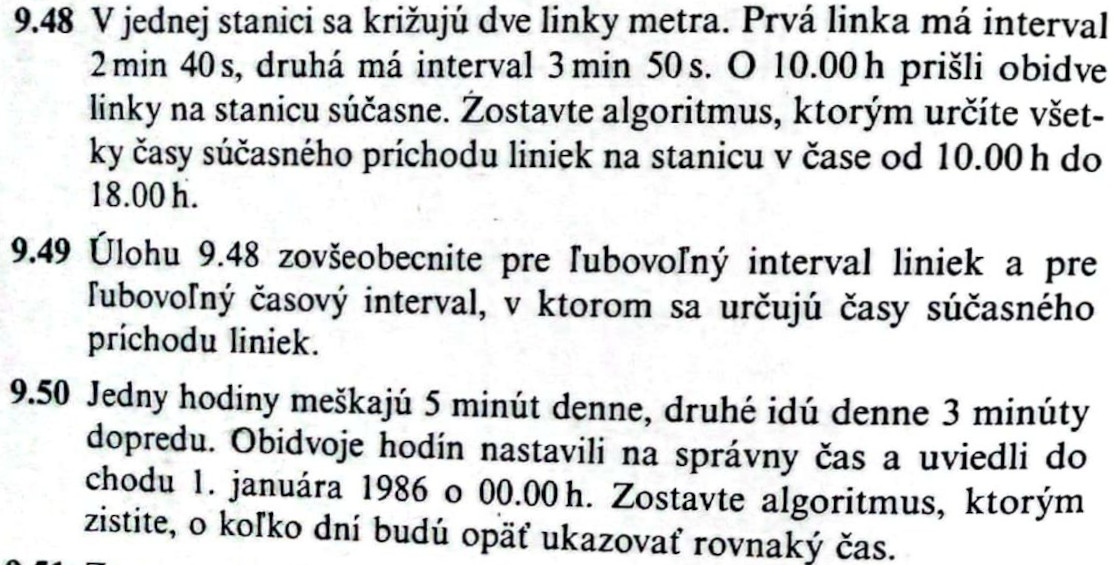
\includegraphics[width=0.9\textwidth]{assets/zbierka-mat-cyklus.jpg}}
\caption{Úlohy na príkaz cyklu}
\end{subfigure}
\caption{Ukážky z kapitoly algoritmy v zbierke úloh z matematiky pre 3. ročník~SŠ}
\label{fig:matematika-slovne-ulohy}
\end{figure}

Odlišný prístup ku grafickej úprave majú knihy zo série ,,Skúsiš to s ...'', v rámci ktorej boli uvedené knihy programovania pre mikropočítače v Basicu a strojovom kóde (\cite{tatchellova_skusis_1990}, \cite{wattsova_skusis_1991}). Cieľové miesta pôsobenia knihy neboli v čase vydania zrejme školy, ale skôr počítačové krúžky ako voľnočasové aktivity. Tieto dve knihy sa nápadite odlišujú pestrofarebnými ilustráciami až takmer komiksovým podtónom, kde sú hlavnými hrdinami roboti v ľudskom a hmyzom stvárnení a mimozemšťania. Krátke odseky výkladového textu sú obohatené o motivovanie každého príkazu jednoduchým príkladom priamo pobádajúcim na odskúšanie (Obr.~\ref{fig:skusis-prog-premenne}). Funkčné bloky kódu rozsiahlejších programov sú priebežne vysveľované textom so svorkami (Obr.~\ref{fig:skusis-prog-kozmicke-bane}), čo môže slúžiť ako dobrý model na prezentovanie riešení v zbierke.

\begin{figure}[h]
\centering
\begin{subfigure}[b]{0.55\textwidth}
\centering
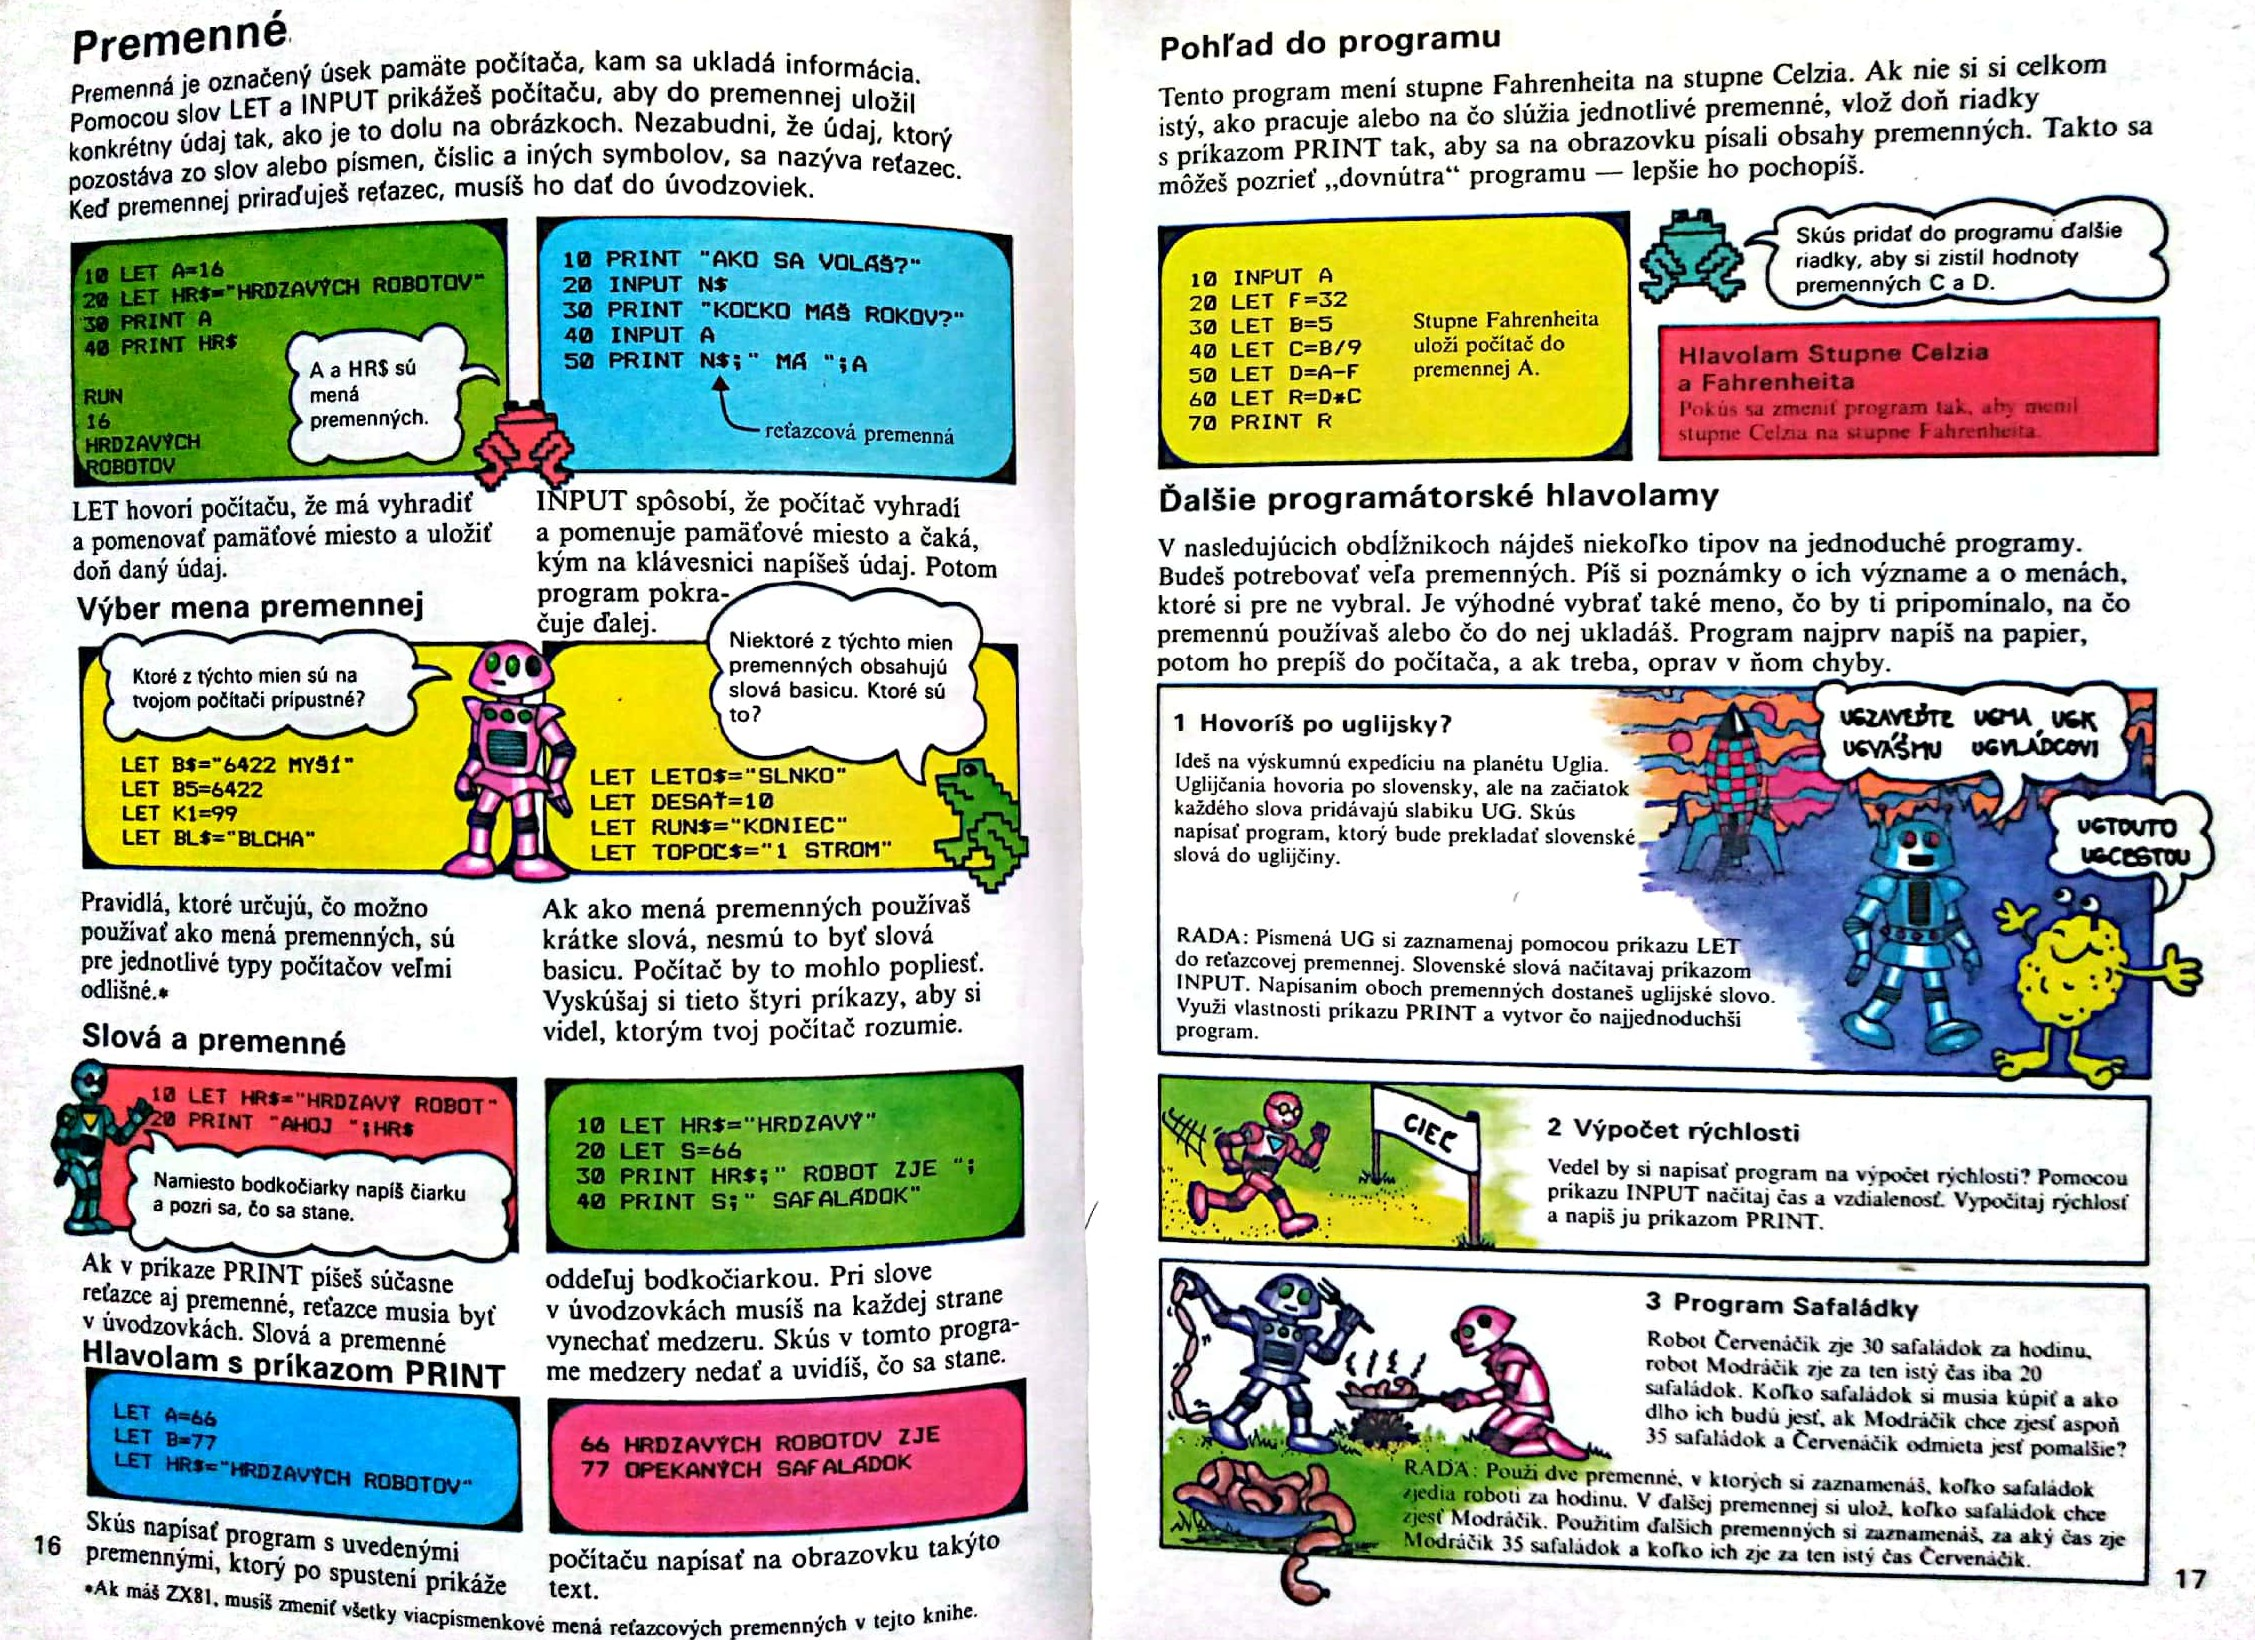
\includegraphics[width=\textwidth]{assets/kniha-premenne.jpg}
\caption{Výkladový text o premenných s hlavolamami}
\label{fig:skusis-prog-premenne}
\end{subfigure}
\hfill
\begin{subfigure}[b]{0.44\textwidth}
\centering
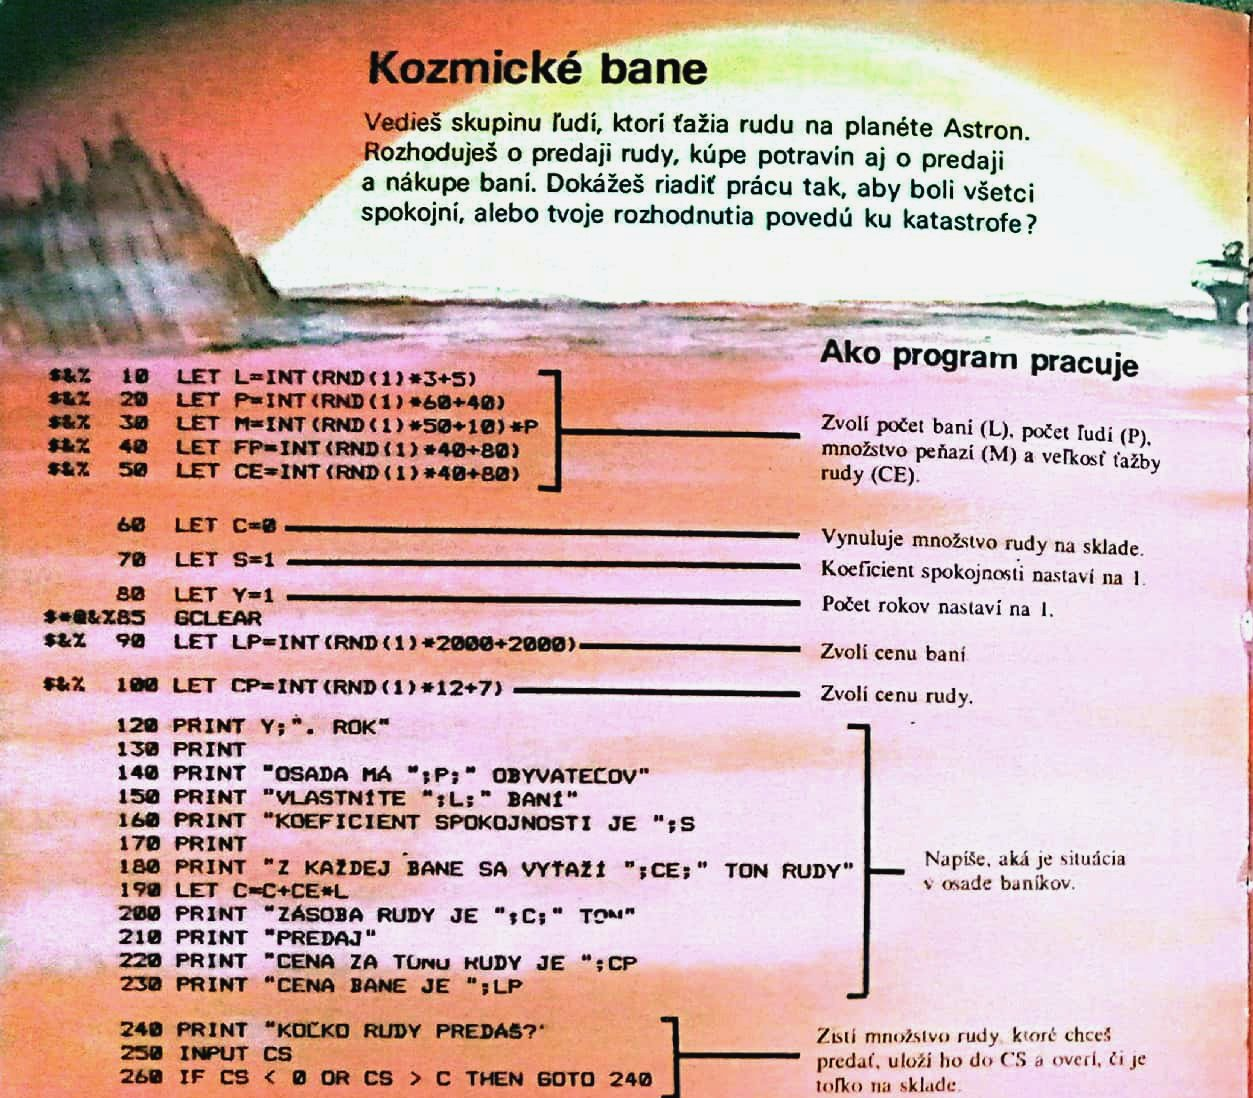
\includegraphics[width=\textwidth]{assets/program-kozmicke-bane.jpg}
\caption{Opis kódu program počítačovej hry}
\label{fig:skusis-prog-kozmicke-bane}
\end{subfigure}
\caption{Bohato ilustrovaná kniha o programovaní v jazyku Basic}
\end{figure}

Učebné texty na webe pod názvom: ,,Algoritmy a programovanie v Pascale: nielen pre maturantov z predmetu informatika'', tvoria obsiahly prierez prvkov programovacieho jazyka konkrétne: výraz s premennou, údajové typy, vetvenie, cyklus, cyklus v cykle, procedúry, funkcie, rekurzia, jednorozmerné polia, textový súbor, vyhľadávanie a triedenie polí, reťazce znakov (\cite{hedvigova_algoritmy_2007}). Učebnica je prehľadne štruktúrovaná. Z obsahu sa hypertextom smeruje na kapitoly, kde je každý nový pojem typograficky zvýraznený podčiarknutím, príkazy jazyka sú odlíšené neproporcionálnym rezom a farbou písma. Po jadre kapitoly nasledujú obvykle 2 vzorové príklady s riešeniami, spravidla 3 priebežné programátorské úlohy (Obr.~\ref{fig:uloha-pascal}), otázky na opakovanie teórie, a úlohy na precvičovanie celej témy. Na konci učebnice je umiestnených 51 jednoduchších úloh na opakovanie a 30 úloh pre náročnejších, ktorým však chýba zmysluplná organizácia náročnosti.

\begin{figure}[h]
\centering
\fbox{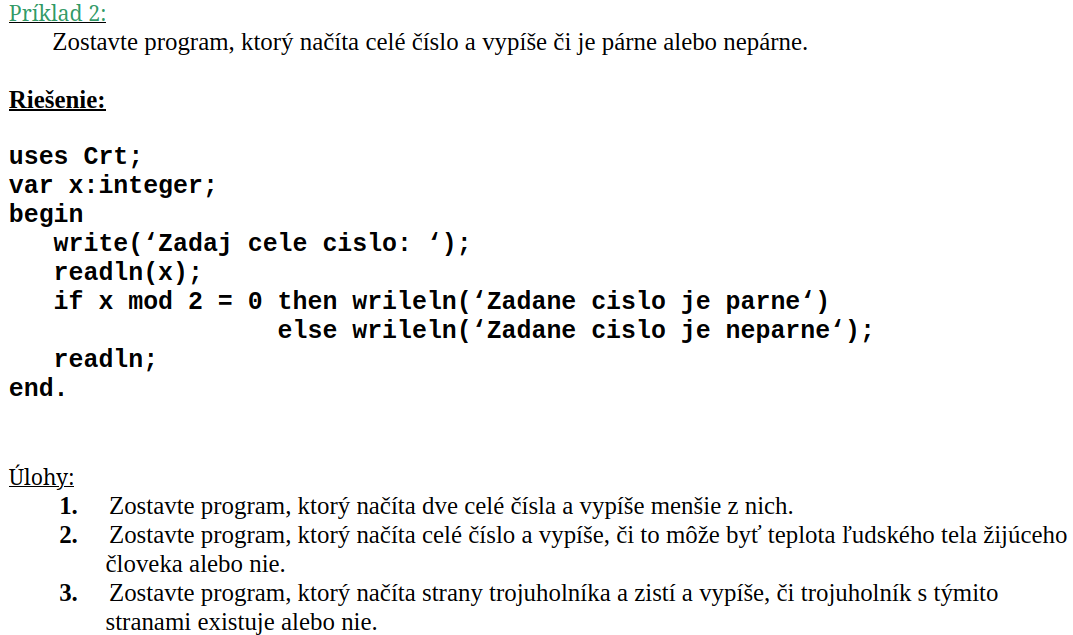
\includegraphics[width=0.8\textwidth]{assets/uloha-pascal.png}}
\caption{Riešený príklad z vetvenia nasledovaný úlohami na samostatnú prácu}
\label{fig:uloha-pascal}
\end{figure}

Slovné úlohy objasňujúci s príbehom  problémové situácie, sú prítomné v súťažiach ako sú Olympiáda v Informatike, organizovanú Národným inštitútom vzdelávania a mládeže, alebo Zenit, Korešpondenčný seminár (KSP) a Letné školy, organizované občianskym združením Trojsten. Vzorové riešenia zadaní vychádzajú v príručkách po skončení kôl. Keďže úlohy bývajú nad rámec základného učiva, tak na vysvetlenie často sa vyskytujúcich algoritmov vznikla tzv. Kuchárka KSP (\cite{noauthor_kucharka_2022}). Ukážka na Obr.~\ref{fig:ksp-oblecenie} ilustruje predlohu pre zadanie z KSP, ktorá sa vyznačuje okrem popisu situácie cez krátky dej, jasným stanovením vstupov a výstupov. 

\begin{figure}[h]
\centering
\fbox{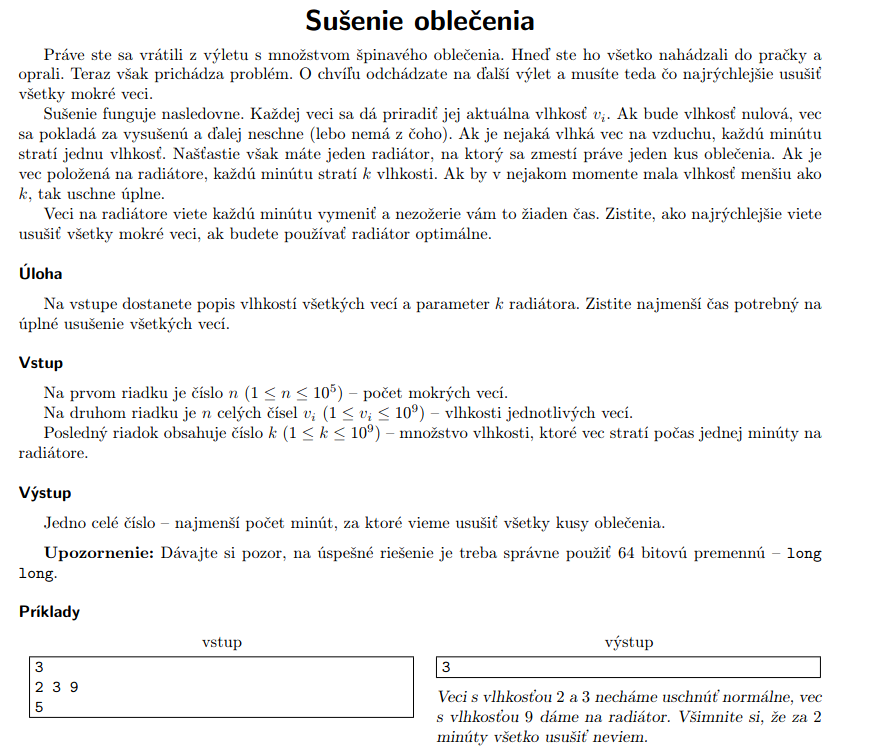
\includegraphics[width=0.8\textwidth]{assets/susenie-oblecenia.png}}
\caption{Úloha letnej školy KSP na binárne vyhľadávanie s úvodným príbehom}
\label{fig:ksp-oblecenie}
\end{figure}

Uvedenie programovacieho jazyka \emph{Python} do výučby informatiky na stredných školách znamenal dopyt po nových učebných materiáloch, ktoré preložia zápisy hlavne z dosiaľ používaného jazyku Pascal. Populatitu nadobudol Python vďaka odstráneniu deklarácie typu premenných a čitateľnejšiemu zápisu, pretože odsadením nahrádza označenie blokov kľúčovými slovami (\emph{begin} a \emph{end}) alebo zloženými zátvorkami. Medzi učebnicami Pythonu prevláda trend predstavovať programovanie cez procedurálne kreslenie cez modul \emph{tkinter}, \emph{turtle}, niekedy \emph{pygame}. V grafickom programovaní sa pojem cyklu prestavuje oveľa skorej ako podmienky, presne naopak než v textovom móde.

Kučera a Výbošťok dali dohromady trojdielnu sériu učebníc ,,Programujeme v Pythone'', v slovenskom a anglickom jazyku so zodpovedajúcimi príručkami pre učiteľov a testami k učebnici. Vypracovali aj zbierku 64 riešených úloh k maturite z informatiky ,,Maturujeme v Pythone''. Vychádzali z potrieb aktívnych učiteľov z Klubu učiteľov vedeného autorom. Osnova prvého diela učebnice začína grafickými príkazmi (Obr.~\ref{fig:kucera-kreslenie-python}) a ďalej sa skladá z premenných, opakovaní častí programu, podprogramov, klikania myšou a ovládaním klávesnicou, podmienených príkazov, časovača a snaženie sa zavŕši tvorbou jednoduchých hier (\cite{kucera_programujeme_2016}). 

\begin{figure}[h]
\centering
\begin{subfigure}[b]{0.55\textwidth}
\centering
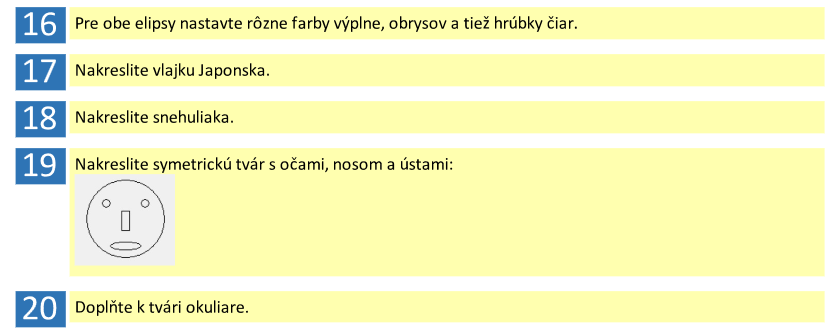
\includegraphics[width=\textwidth]{assets/kucera-python.png}
\caption{Kreslenie obdĺžníkov}
\label{fig:kucera-kreslenie-python}
\end{subfigure}
\begin{subfigure}[b]{0.44\textwidth}
\centering
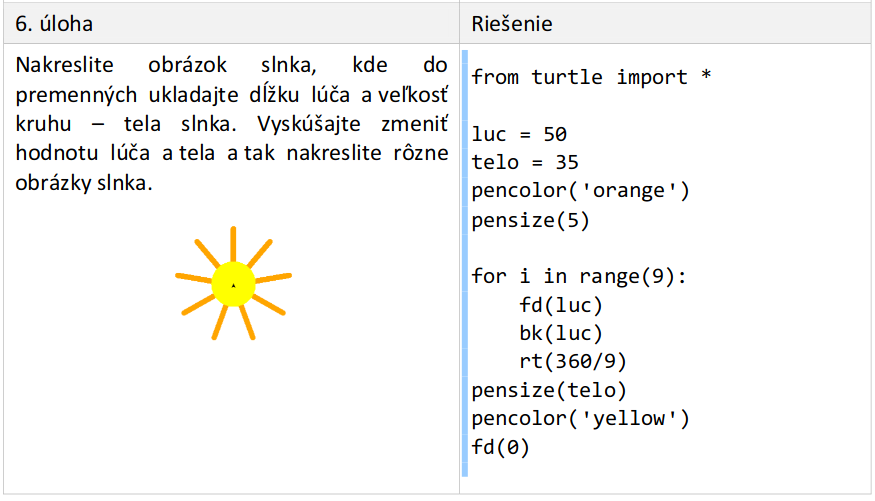
\includegraphics[width=\textwidth]{assets/uloha-turtle.png}
\caption{Cyklus a korytnačia grafika}
\label{fig:turtle-graphics}
\end{subfigure}
\caption{Úlohy na programovanie grafiky v jazyku Python}
\end{figure}

Blaho a Salanci pripravili pracovné listy \emph{abcPython} na 20 vyučovacích hodín, kde nepočítajú s výkladom učiteľa. Dostupné sú aj metodické materiály ku listom. Preberajú sa postupne témy kde sa prelína textový a grafický režim: interaktívny zadávanie príkazov, výrazy, premenné, výpisy, kreslenie, náhoda, výrazy v cykle, elipsy, vetvenie, podprogramy, kreslenie myšou (\cite{blaho_abcpython_2019}, \cite{blaho_metodiky_2019}). 

Mészárosová vytvorila metodickú príručku pre vyučovanie základov programovania, kde cez Python rozvíja na rozpätí 16 vyučovacích hodín korytnačiu grafiku (Obr.~\ref{fig:turtle-graphics}). Využíva tým oboznámenosť žiakov s korytnačkami v jazyku Logo z druhého stupňa základnej školy. Rovnako sa začína predstavením grafickými pokynov na pohyb a kreslenie korytnačkou. Nasledujú premenné, for cyklus, funkcie, funkcie s parametrami, poloha korytnačky, náhodná poloha, vetvenie a na upevnenie zručností slúži projekt kreslenia pohľadnice (\cite{meszarosova_python_2017}).



\chapter{Cieľ a metodika práce}
Cieľom záverečnej práce je zostaviť rozšíriteľnú \textbf{zbierku úloh z programovania} so vzorovými riešeniami v predmete informatika pre stredné školy. Primárny zámer súčasne vyžaduje uspokojenie nasledujúcich požiadaviek na navrhnutý systém úloh pre pedagogickú prax:

\begin{itemize}[noitemsep]
\item pokrytie základného učiva v súlade so ŠVP a cieľovými požiadavkami
\item poskytnutie metodiky na spôsob zaradenia ďalších úloh do nášho systému úloh
\item čitateľnosti textu zadaní primeranej žiakom vo veku 15 - 18 rokov
\item príbehovosť opisu problémovej situácie v znení zadania
\item vzorové riešenia v programovacom jazyku Python
\item zobrazenie na webovej stránke s efektívnym využitím hypertextu
\end{itemize}

Splnenie vytýčených cieľov sa opiera o rešerš informačných zdrojov vyhľadaných prostredníctvom plnotextových vyhľadávačov webu a knižníc, na základe rád školiteľky a osobného povedomia o oblasti. Knihy a články boli podrobené procesu analýzy, kedy sa vyselektovali relevantné definície, charakteristiky, kategorizácie a postupy. Metóde porovnania sa podrobili existujúce učebné texty základov programovania.

Vlastná tvorba zbierky úloh prebiehala syntézou psychologických východísk porozumenia textu, známych typových úloh a známej metodiky na preformulovanie úloh. Hodnotenie kvality textu úloh v zbierke sa uskutočnilo kvantitatívne i kvalitatívne. Úroveň čitateľnosti sa indikatívne vyčíslila pomocou Gunning fog indexu (Vzorec~\ref{equ:fog-index}). Kvalitatívne sa pozorovali problémy  žiakov pri riešenia úloh v zbierke na vyučovacej hodine plynúcej z neporozumenia formulácie zadania. Metodika klasifikácie úlohy v systéme vychádza z kritérií témy, podtémy, elementu, didaktickej funkcie a kognitívnej úrovne podľa Minďákovej (Sekcia~\ref{sec:klasifikacia-ulohy}).


\chapter{Výsledky práce}
%TODO


Výsledky (vlastné postoje alebo vlastné riešenie vecných problémov), ku ktorým autor dospel, sa musia logicky usporiadať a pri popisovaní sa musia dostatočne zhodnotiť. Zároveň sa komentujú všetky skutočnosti a poznatky v konfrontácii s výsledkami iných autorov. 

\section{Zbierka úloh}
medzipredmetové vzťahy: matematika, fyzika, finančná gramotnosť, chémia, dejepis, geografia

zoradené podľa obtiažnosti: 

1. Premenné - 11 úloh
2. Podmienky - 9 úloh
3. Cykly - 9 úloh
4. Náhodné čísla - 3 úlohy
5. Zoznamy - 9 úloh
6. Súbory - 6 úloh
7. Funkcie - 11 úloh

\subsection{Premenné}
\underline{\textbf{Premenná}} je taká krabička na odkladanie čísel alebo slov, ktoré si potrebujeme zapamätať na dokončenie činnosti. Premenné sa líšia svojim \underline{\textbf{dátovým typom}}. Premenná dostane svoj typ cez \underline{\textbf{priradenie}}, čiže vtedy keď prvýkrát do nej niečo uložíme. Typ hovorí o tom, čo sa vo vnútri premennej nachádza.

Základné typy premenných sú:
\begin{itemize}[noitemsep,topsep=0pt]
\item \underline{\textbf{Logická hodnota}} (\textit{bool}) - môže mať len dve hodnoty - pravda (\textit{True}) alebo nepravda (\textit{False})
\item \underline{\textbf{Celé číslo}} (\textit{int}) - ukladáme sem ľubovolné kladné a záporné celé čísla (\textit{97})
\item \underline{\textbf{Desatinné číslo}} (\textit{float}) - Líšia sa od celých čísel spôsobom uloženia (\textit{3.14159})
\item \underline{\textbf{Reťazec}} (\textit{str}) - Označujeme ich úvodzovkami alebo apostrofmi a väčšinou predstavujú text napísaný na klávesnici alebo zobrazený na obrazovke \textit{``Učím sa programovať!''}).
\end{itemize}

\subsubsection*{1. Pozdrav}
Skladáš si stavebnicu robotického domáceho miláčika, ktorý je takmer dokonalý. Má telo, končatiny, hlavu a vie kráčať po stole. Keby však sa naučil aj hovoriť, to by bol potom poriadny spoločník. Každý dobrý rozhovor sa začína pozdravom. Napíš program, ktorý ťa pozdraví po napísaní mena na klávesnici. Doplň tiež, aby sa program s tebou aj rozlučil.

\begin{tabular}{@{}p{0.15\linewidth}p{0.75\linewidth}}
\textbf{\small Vstup:} &
\vspace{-3em}
\begin{code}
Ako sa voláš?: @\fbox{\phantom{meno}}@
\end{code}
\end{tabular}

\vspace{-2em}
\begin{tabular}{@{}p{0.15\linewidth}p{0.75\linewidth}}
\textbf{\small Výstup:} &
\vspace{-3em}
\begin{code} 
Ahoj @\fbox{\phantom{meno}}@
\end{code}
\end{tabular}
\vspace{-2em}

\subsubsection*{2. Básnik}
Rozkríklo sa, že píšeš pekné básničky na rôzne príležitosti. Prichádza ti čím ďalej viac prosieb od kamarátov a známych, či im nevytoríš peknú rýmovačku. Vymýšať kreatívne texty je niekedy veľká námaha, tak ti napadne, že stačí meniť len rým. Napíš program, ktorý za teba slovo vloží do predlohy básne.

\begin{tabular}{@{}p{0.15\linewidth}p{0.75\linewidth}}
\textbf{\small Vstup:} &
\vspace{-3em}
\begin{code}
Napíš slovo, ktoré sa rýmuje so slovom strach: @\fbox{\phantom{slovo}}@
\end{code}
\end{tabular}

\vspace{-2em}
\begin{tabular}{@{}p{0.15\linewidth}p{0.75\linewidth}}
\textbf{\small Výstup:} &
\vspace{-3em} 
\begin{code}
Tu je báseň:
Z počítačov mával som vždy strach,
teraz som však šťastný ako @\fbox{\phantom{slovo}}@.
\end{code}
\end{tabular}
\vspace{-2em}

\subsubsection*{3. Pozvánka}
Budúci víkend organizuješ velkolepú narodeninovú párty a rozposielaš na ňu pozvánky. Okrem mena hosťa potrebuješ meniť aj čas konania oslavy. Máš totiž skúsenosti, že nie všetci chodia načas. Každý pozvaný si má priniesť okrem darčeku aj jednu špeciálnu vec. Napíš program, ktorý doplní takúto pozvánku na mieru.

\begin{tabular}{@{}p{0.15\linewidth}p{0.75\linewidth}}
\textbf{\small Vstup:} &
\vspace{-3em}
\begin{code}
Meno kamaráta: @\fbox{\phantom{vstup}}@
Čas oslavy: @\fbox{\phantom{vstup}}@
Prinesie okrem darčeku: @\fbox{\phantom{vstup}}@
\end{code}
\end{tabular}

\vspace{-2em}
\begin{tabular}{@{}p{0.15\linewidth}p{0.75\linewidth}}
\textbf{\small Výstup:} &
\vspace{-3em} 
\begin{code}
Ahoj @\fbox{\phantom{vstup}}@,
pozývam ťa na moju narodeninovú párty.
Bude sa konať 12.4. o @\fbox{\phantom{vstup}}@. 
Nezabudni priniesť @\fbox{\phantom{vstup}}@ a pekný darček.
Teším sa na teba! :)
\end{code}
\end{tabular}
\vspace{-2em}

\subsubsection*{4. Teplota vo Farenheitoch}
Prišiel si na dovolenku do Spojených štátov amerických. Obliekaš sa na krátky výlet von, ale nevieš ako sa máš obliecť. Na teplomeroch sú napísané len stupne Fahrenheita. Napíš program, ktorý ich premení na stupne Celzia s presnosťou na dve desatinné miesta.

\begin{tabular}{@{}p{0.15\linewidth}p{0.75\linewidth}}
\textbf{\small Vstup:} &
\vspace{-3em}
\begin{code}
Vonku je °F: @\fbox{\phantom{vstup}}@
\end{code}
\end{tabular}

\vspace{-2em}
\begin{tabular}{@{}p{0.15\linewidth}p{0.75\linewidth}}
\textbf{\small Výstup:} &
\vspace{-3em} 
\begin{code}
Doma by bolo na teplomeri @\fbox{\phantom{vstup}}@°C.
\end{code}
\end{tabular}
\vspace{-2em}

\subsubsection*{5. Hlboká roklina}
Stojíš nad hlbokým údolím za zábradlím a uvažuješ ako odmerať jeho hĺbku. Vtom si spomenieš na svoje vedomosti z fyziky. Zoberieš si do ruky povaľúci sa kameň a pustíš ho priamo do rokliny. Zároveň stlačíš stopky, ktorými zmeriaš čas do dopadu v sekundách. Kameň padá nadol voľným pádom. Stopky zastaviš pri započutí rachotu z nárazu. Pri výpočte zanedbáme rýchlosť zvuku, ktorou sa rachot rožšíri až k nám.

\begin{tabular}{@{}p{0.15\linewidth}p{0.75\linewidth}}
\textbf{\small Vstup:} &
\vspace{-3em}
\begin{code}
Čas do dopadu kameňa: @\fbox{\phantom{vstup}}@
\end{code}
\end{tabular}

\vspace{-2em}
\begin{tabular}{@{}p{0.15\linewidth}p{0.75\linewidth}}
\textbf{\small Výstup:} &
\vspace{-3em}
\begin{code}
Hĺbka rokliny je @\fbox{\phantom{vstup}}@ metrov.
\end{code}
\end{tabular}
\vspace{-2em}

\subsubsection*{6. Vedro s vodou}
V rodinnom dome ste ekologicky uvedomelí, lebo zachytávate ďaždovú vodu z odkvapu na polievanie záhrady. Minulú noc vám napršalo do nádrže veľa vody. Keď bude o pár dní suchšie mama ťa pošle poliať rastliny uzavretým vedrom valcového tvaru. To naplníš vždy až po okraj. Zaujíma ťa, aký objem naberieš na jedno naplnenie. Rozmery valcového vedra vieš odmerať pravítkom. Napíš program, ktorý zráta koľko sa zmestí vody do rôzne veľkých vedier.

\begin{tabular}{@{}p{0.15\linewidth}p{0.75\linewidth}}
\textbf{\small Vstup:} &
\vspace{-3em}
\begin{code}
Výška vedra (cm): @\fbox{\phantom{vstup}}@
Priemer dna (cm): @\fbox{\phantom{vstup}}@
\end{code}
\end{tabular}

\vspace{-2em}
\begin{tabular}{@{}p{0.15\linewidth}p{0.75\linewidth}}
\textbf{\small Výstup:} &
\vspace{-3em}
\begin{code}
Do vedra sa zmestí @\fbox{\phantom{vstup}}@ litrov vody.
\end{code}
\end{tabular}
\vspace{-2em}

\subsubsection*{7. Cesta autom}
Tešíš sa na očakávaný výlet autom po Európe. Pri plánovaní trasy chceš zistiť akou rýchlosťou musíte priemerne cestovať, aby ste od rána stihli navštíviť všetky miesta. Večer však musíte prísť včas do hotela, aby vás ubytovali. Napíš program, ktorý ti s tým pomôže.

\begin{tabular}{@{}p{0.15\linewidth}p{0.75\linewidth}}
\textbf{\small Vstup:} &
\vspace{-3em}
\begin{code}
Dĺžka cesty (km): @\fbox{\phantom{vstup}}@
Odchod z domu (hodina): @\fbox{\phantom{vstup}}@
Príchod do hotela (hodina): @\fbox{\phantom{vstup}}@
\end{code}
\end{tabular}

\vspace{-2em}
\begin{tabular}{@{}p{0.15\linewidth}p{0.75\linewidth}}
\textbf{\small Výstup:} &
\vspace{-3em}
\begin{code}
Auto pôjde priemernou rýchlosťou @\fbox{\phantom{vstup}}@ km/h.
\end{code}
\end{tabular}
\vspace{-2em}

\subsubsection*{8. Kúpalisko}
Začína sa horúca letná sezóna. Prevádzka kúpaliska musí pred otvorením napustiť bazény. Všetky bazény v areáli sú kvádrového tvaru, ktorých rozmery poznáme. Vedúceho kúpaliska zaujíma spotrebovaná voda pre bazén, keď bude napustený pod okraj. Voda nie je zadarmo, preto si chcú pripraviť dosť peňazí, aby za ňu zaplatili.

\begin{tabular}{@{}p{0.15\linewidth}p{0.75\linewidth}}
\textbf{\small Vstup:} &
\vspace{-3em}
\begin{code}
Dĺžka bazéna (m): @\fbox{\phantom{vstup}}@
Šírka bazéna (m): @\fbox{\phantom{vstup}}@
Hĺbka bazéna (m): @\fbox{\phantom{vstup}}@
Hĺbka hladiny pod okrajom (cm): @\fbox{\phantom{vstup}}@
Cena za m^3 vody v eurách: @\fbox{\phantom{vstup}}@ 
\end{code}
\end{tabular}

\vspace{-2em}
\begin{tabular}{@{}p{0.15\linewidth}p{0.75\linewidth}}
\textbf{\small Výstup:} &
\vspace{-3em}
\begin{code}
Na bazén sa minie @\fbox{\phantom{vstup}}@ litrov vody.
Voda bude stáť @\fbox{\phantom{vstup}}@ eur.
\end{code}
\end{tabular}
\vspace{-2em}

\subsubsection*{9. Maľovanie}
S rodičmi sa sťahuješ do nového bytu. Dali ti za úlohu kúpiť si farbu na vymaľovanie izby. Nástroj na rýchle počítanie množstva farby by sa hodil asi aj profesionálnym maliarom. Vytvor program na vypočítanie plochy stien a stropu bez okna a podlahy.

\begin{tabular}{@{}p{0.15\linewidth}p{0.75\linewidth}}
\textbf{\small Vstup:} &
\vspace{-3em}
\begin{code}
Rozmery miestnosti
Dĺžka (cm): @\fbox{\phantom{vstup}}@
Šírka (cm): @\fbox{\phantom{vstup}}@
Výška (cm): @\fbox{\phantom{vstup}}@
Rozmery okna
Šírka (cm): @\fbox{\phantom{vstup}}@
Výška (cm): @\fbox{\phantom{vstup}}@
Výdatnosť farby (m^2/kg): @\fbox{\phantom{vstup}}@
\end{code}
\end{tabular}

\vspace{-2em}
\begin{tabular}{@{}p{0.15\linewidth}p{0.75\linewidth}}
\textbf{\small Výstup:} &
\vspace{-3em}
\begin{code}
Maľovať budeš plochu @\fbox{\phantom{vstup}}@ m^2. 
Kúp @\fbox{\phantom{vstup}}@ kg farby.
\end{code}
\end{tabular}
\vspace{-2em}

\subsubsection*{10. Chemikálie}
Chemici v laboratóriu bežne zmiešavajú roztoky, aby dosiahli správny pomer želanej látky. Roztoky sú opísané svojou hmotnosťou ($m$) a hmotnostným zlomkom rozpustenej látky v rozpúštadle ($w$). Viaceré látky odlíšime dolným indexom ($m_1$).  Hmotnosť sa uvádza v gramoch a hmotnostný zlomok v percentách. Napíš program na opísanie vlastností výsledného roztoku. Na výpočet použi tieto rovnice:
\begin{align*}
m_3 &= m_1 + m_2 \\
m_3 \cdot w_3 &= m_1 \cdot w_1 +  m_2 \cdot w_2
\end{align*}

\begin{tabular}{@{}p{0.15\linewidth}p{0.75\linewidth}}
\textbf{\small Vstup:} &
\vspace{-3em}
\begin{code}
Hmotnosť roztoku č.1 (m1)? @\fbox{\phantom{vstup}}@
Hmotnostný zlomok roztoku č.1 (w1)? @\fbox{\phantom{vstup}}@
Hmotnosť roztoku č.2 (m2)? @\fbox{\phantom{vstup}}@
Hmotnostný zlomok roztoku č.2 (w2)? @\fbox{\phantom{vstup}}@
\end{code}
\end{tabular}

\vspace{-2em}
\begin{tabular}{@{}p{0.15\linewidth}p{0.75\linewidth}}
\textbf{\small Výstup:} &
\vspace{-3em}
\begin{code}
Výsledný roztok má hmotnosť @\fbox{\phantom{vstup}}@ g.
Hmotnostný zlomok rozpustenej látky je @\fbox{\phantom{vstup}}@ %.
\end{code}
\end{tabular}
\vspace{-2em}

\subsubsection*{11. Brzdenie}
V poslednej dobe sa objavuje na trati viac nebezpečných zrážok. Rušňovodiči ťa požiadali, aby si zistil ako rýchlo a ďaleko pred prekážkou dokáže vlak zastaviť. Vlaková súprava ide pred brzdením svojou stálou rýchlosťou v kilometroch za hodinu. Hmotnosť vlaku tvorí súčet hmotností lokomotívy a všetkých vagónov. Brzdy na kolesách majú spoločnú brzdnú silu uvedenú v Newtonoch na tonu. V programe využiješ nasledovné fyzikálne vzťahy:

\begin{itemize}
\itemsep0pt
\item Kinetická energia pohybujúceho sa vlaku (práca potrebná na zabrzdenie): \\ $ W = E_k = \frac{1}{2} \cdot m \cdot v^2 $
\item Brzdná dráha pri brzdnej sile $F_b$: $s = \frac{W}{F_b \cdot m} $
\item Čas na zastavenie vlaku pri rovnomernom spomalenom pohybe: $ t = \sqrt{\frac{2 \cdot s}{F / m}} $
\end{itemize}

\begin{tabular}{@{}p{0.15\linewidth}p{0.75\linewidth}}
\textbf{\small Vstup:} &
\vspace{-3em}
\begin{code}
Vlaková súprava
- Rýchlosť (km/h): @\fbox{\phantom{vstup}}@
- Hmotnosť lokomotívy (t): @\fbox{\phantom{vstup}}@
- Hmotnosť vagóna (t): @\fbox{\phantom{vstup}}@
- Počet vagónov: @\fbox{\phantom{vstup}}@
- Brzdná sila (N/t): @\fbox{\phantom{vstup}}@
\end{code}
\end{tabular}

\vspace{-2em}
\begin{tabular}{@{}p{0.15\linewidth}p{0.75\linewidth}}
\textbf{\small Výstup:} &
\vspace{-3em}
\begin{code}
Vlaková súprava má hmotnosť @\fbox{\phantom{vstup}}@ ton.
V rýchlosti @\fbox{\phantom{vstup}}@ km/h zabrzdí na vzdialnosť @\fbox{\phantom{vstup}}@ metrov.
Brzdenie bude trvať @\fbox{\phantom{vstup}}@ sekúnd.
\end{code}
\end{tabular}
\vspace{-2em}
 

\subsection{Podmienky}
\underline{\textbf{Podmienky}} sú ako križovatky na ceste. Podľa toho kam chceme ísť, sa rozhodneme, ktorou cestou pôjdeme ďalej. Aby sme sa uistili, že máme ten správny smer (\underline{\textbf{vetva podmienky}}) pýtame sa vždy logickú otázku. Otázka používa údaje uložené v premenných.

\subsubsection*{1. Heslo}
Tvoj dom na strome už vykradlo pár nezvaných návštevníkov. Vymyslel si preto spôsob ako dovoliť návštevu len overeným osobám. Tie musia poznať tajné heslo. Napíš program, ktorý slovne privíta členov a odoženie zlodejov.

\begin{tabular}{@{}p{0.15\linewidth}p{0.75\linewidth}}
\textbf{\small Vstup:} &
\vspace{-3em}
\begin{code}
Stoj! Povedz Heslo!
? @\fbox{\phantom{vstup}}@
\end{code}
\end{tabular}

\vspace{-2em}
\begin{tabular}{@{}p{0.15\linewidth}p{0.75\linewidth}}
\textbf{\small Výstup:} &
\vspace{-3em}
\begin{code}
Vstúp, priateľ 
(alebo Zmizni kade ľahšie)
\end{code}
\end{tabular}
\vspace{-2em}

\subsubsection*{2. Najväčšie číslo}
Na lúke sa hrajú šípky. Hrači si zapisujú dosiahnuté skóre na tabuľu. Dnes proti sebe hrali v partii traja protihráči. Napíš program, ktorý označí hráča s najväčším získaným počtom bodov.

\begin{tabular}{@{}p{0.15\linewidth}p{0.75\linewidth}}
\textbf{\small Vstup:} &
\vspace{-3em}
\begin{code}
1.skóre: @\fbox{\phantom{vstup}}@
2.skóre: @\fbox{\phantom{vstup}}@
3.skóre: @\fbox{\phantom{vstup}}@
\end{code}
\end{tabular}

\vspace{-2em}
\begin{tabular}{@{}p{0.15\linewidth}p{0.75\linewidth}}
\textbf{\small Výstup:} &
\vspace{-3em}
\begin{code}
Najväčie skóre @\fbox{\phantom{vstup}}@ bodov má @\fbox{\phantom{vstup}}@ hráč.
\end{code}
\end{tabular}
\vspace{-2em}


\subsubsection*{3. Vhodné oblečenie}
Módni poradcovia vyšli z módy a ich prácu prebrali počítače. Na základe počasia a príležitosti odporúčajú vhodný outfit. Vymysli pár tipov pre rôzne situácie a začni radiť.

\begin{tabular}{@{}p{0.15\linewidth}p{0.75\linewidth}}
\textbf{\small Vstup:} &
\vspace{-3em}
\begin{code}
Ako je vonku?: @\fbox{\phantom{vstup}}@
Kam ideš?: @\fbox{\phantom{vstup}}@
\end{code}
\end{tabular}

\vspace{-2em}
\begin{tabular}{@{}p{0.15\linewidth}p{0.75\linewidth}}
\textbf{\small Výstup:} &
\vspace{-3em}
\begin{code}
Určite si nezabudni @\fbox{\phantom{vstup}}@ a tiež si vezmi @\fbox{\phantom{vstup}}@.
\end{code}
\end{tabular}
\vspace{-2em}

\subsubsection*{4. Morský vánok}
Kapitán plachetnice na otvorenom oceáne musí mať vždy prehľad odkiaľ fúka vietor, aby dokormidloval do vytúženého cieľa. Príliš silné závany vetra môžu byť nebezpečné pre posádku. Rozthať polámať lodné sťažne, potrhať plachty, či zaplaviť palubu. Cez rádio dostáva plavidlo každý deň správy o predpovedi sily vetra v Beafortovej stupnici. Sila vetra je ňou vyjadrená do dvanástich stupňov od bezvetria až po orkán. Napíš program, ktorý kapitánu vysvetlí stupeň vetra. Podľa stupnice určíme jeho pomenovanie, rýchlosti v námorných uzloch a očakávateľnej výšky vĺn.

\begin{tabular}{@{}p{0.15\linewidth}p{0.75\linewidth}}
\textbf{\small Vstup:} &
\vspace{-3em}
\begin{code}
Sila vetra na Beaufortovej stupnici: @\fbox{\phantom{12}}@
\end{code}
\end{tabular}

\vspace{-2em}
\begin{tabular}{@{}p{0.15\linewidth}p{0.75\linewidth}}
\textbf{\small Výstup:} &
\vspace{-3em}
\begin{code}
Vietor sa nazýva @\fbox{\phantom{vstup}}@.
Vietor má rýchlosť @\fbox{\phantom{vstup}}@ kt.
Očakávaná výška vĺn je @\fbox{\phantom{vstup}}@ m.
\end{code}
\end{tabular}
\vspace{-2em}


\subsubsection*{5. Pokazený rozpis}
Továreň na železnú rudu dostala nový časový rozpis vylepšeného technologického procesu. Spracovanie zvyčajne trvá dlhšie ako hodinu. Nehodí sa im teda mať časy napísané iba v minútach. Rozpíš programom minúty na dni, hodiny, minúty pre jednoduchšie čítanie rozpisu. Vynechaj nepotrebné časové údaje.

\begin{tabular}{@{}p{0.15\linewidth}p{0.75\linewidth}}
\textbf{\small Vstup:} &
\vspace{-3em}
\begin{code}
Trvanie (min.): @\fbox{\phantom{vstup}}@
\end{code}
\end{tabular}

\vspace{-2em}
\begin{tabular}{@{}p{0.15\linewidth}p{0.75\linewidth}}
\textbf{\small Výstup:} &
\vspace{-3em}
\begin{code}
= @\fbox{\phantom{vstup}}@ d. @\fbox{\phantom{vstup}}@ hod. @\fbox{\phantom{vstup}}@ min.
\end{code}
\end{tabular}
\vspace{-2em}


\subsubsection*{6. Hovoriaca kalkulačka}
Výpočty neboli nikdy väčšia zábava. Teda aspoň s kalkulačkou, ktorá namiesto čudných matematických čmáraníc hovorí ľudskou rečou. Vytvor program pre kalkulačku, ktorá si vypýta dve čísla. Tie bude ich vedieť sčítať alebo odčítať podľa slovného pokynu.

\begin{tabular}{@{}p{0.15\linewidth}p{0.75\linewidth}}
\textbf{\small Vstup:} &
\vspace{-3em}
\begin{code}
Som hovorica kalkulačka a rada počítam!
Povedz mi prvé číslo: @\fbox{\phantom{vstup}}@
Potrebujem ďašie číslo: @\fbox{\phantom{vstup}}@
Chceš ich sčítať alebo odčítať: @\fbox{\phantom{vstup}}@ (sčítať alebo odčítať)
\end{code}
\end{tabular}

\vspace{-2em}
\begin{tabular}{@{}p{0.15\linewidth}p{0.75\linewidth}}
\textbf{\small Výstup:} &
\vspace{-3em}
\begin{code}
Výsledok tvojho príkladu: @\fbox{\phantom{vstup}}@ (plus alebo mínus) @\fbox{\phantom{vstup}}@ je @\fbox{\phantom{vstup}}@.
\end{code}
\end{tabular}
\vspace{-2em}

\subsubsection*{7. Chaos v lístkoch}
Vyznať sa v linkách mestskej hromadnej dopravy si vyžaduje dlhoročné skúsenosti. Treba oplývať aj riadnou dávkou trpezlivosti. Ľahko sa nám stane, že omylom nasadneme do autobusu a hneď sa vydáme na okružnú jazdu po siedmich divoch sídliska. Horší zážitok je stretnutie revízora po zistení, že máme nesprávny lístok alebo že nemáme žiaden ... Postávaš pri automate na lístky a nevieš sa vysomáriť z množstva časov a zón v ponuke. Napíš program, ktorý podľa počtu zónu a trvania ceny vypíše cenu zľavneného lístka. Nájdi na internete aktuálnu tarifu MHD v tvojom meste.

\begin{tabular}{@{}p{0.15\linewidth}p{0.75\linewidth}}
\textbf{\small Vstup:} &
\vspace{-3em}
\begin{code}
Popíš mi svoju cestu s MHD
Koľko zón prejdeš?: @\fbox{\phantom{vstup}}@
Koľko minút má trvať cesta?: @\fbox{\phantom{vstup}}@
\end{code}
\end{tabular}

\vspace{-2em}
\begin{tabular}{@{}p{0.15\linewidth}p{0.75\linewidth}}
\textbf{\small Výstup:} &
\vspace{-3em}
\begin{code}
Zlavnený lístok stojí @\fbox{\phantom{vstup}}@ eur.
\end{code}
\end{tabular}
\vspace{-2em}


\subsubsection*{8. Kvadratická rovnica}
Matematika v škole dokáže byť poriadna otrava. Hlavne, keď od rána do večera nič iné nerobíš ako počítaš príklady na kvadratické rovnice. ,,Načo mám ten počítač'', pomyslíš si večer vo svetle stolnej lampy. Pre zadané koeficienty $a$, $b$, $c$ predpisu $ax^2 + bx + c = 0$ napíš program, ktorý vypočíta jej korene a vrchol paraboly.

\begin{tabular}{@{}p{0.15\linewidth}p{0.75\linewidth}}
\textbf{\small Vstup:} &
\vspace{-3em}
\begin{code}
Koeficienty kvadratickej rovnice:
a = @\fbox{\phantom{vstup}}@
b = @\fbox{\phantom{vstup}}@
c = @\fbox{\phantom{vstup}}@
\end{code}
\end{tabular}

\vspace{-2em}
\begin{tabular}{@{}p{0.15\linewidth}p{0.75\linewidth}}
\textbf{\small Výstup:} &
\vspace{-3em}
\begin{code}
@\fbox{\phantom{a}}@x^2 + @\fbox{\phantom{b}}@x + @\fbox{\phantom{c}}@ = 0
x1 = @\fbox{\phantom{abc}}@
x2 = @\fbox{\phantom{abc}}@
V[@\fbox{\phantom{abc}}@; @\fbox{\phantom{abc}}@]
\end{code}
\end{tabular}
\vspace{-2em}


\subsubsection*{9. Trojuholníky}
Trojuholník je mýtická bytosť, o ktorej je vždy treba zistiť. Nesmieme použiť pravítko, lebo to by nás čakala príliš jednoduchá výzva. Veď bez rysovania zístíme o tejto trojcípej paráde všeličo. Hoci aj keď jej chýbajú niektoré rozmery.

\begin{enumerate}[label=\alph*)]
\item Ak je to možné, doplň chýbajúce informácie pre ľubovoľný trojuholník (zadaný ako SSS) ako sú dĺžky strán a výšok, veľkosti uhlov, obsah a obvod. Využi trojuholníkovú nerovnosť, sínusovú vetu, kosínusovú vetu a vzorec na výpočet obsahu trojuholníkov.
\item Rozšír program aj pre ostatné vety o trojuholníkoch: SUS, USU, UUS.
\end{enumerate}

\begin{tabular}{@{}p{0.15\linewidth}p{0.75\linewidth}}
\textbf{\small Vstup:} &
\vspace{-3em}
\begin{code}
Zadajte strany ľubovolného trojuholníka:
a = @\fbox{\phantom{vstup}}@
b = @\fbox{\phantom{vstup}}@
c = @\fbox{\phantom{vstup}}@
\end{code}
\end{tabular}

\vspace{-2em}
\begin{tabular}{@{}p{0.15\linewidth}p{0.75\linewidth}}
\textbf{\small Výstup:} &
\vspace{-3em}
\begin{code}
Strany: a = @\fbox{\phantom{abc}}@; b = @\fbox{\phantom{abc}}@; c = ___
Uhly: alpha = @\fbox{\phantom{abc}}@°; beta = @\fbox{\phantom{abc}}@°; gamma = @\fbox{\phantom{vstup}}@°
Výšky: v(a) = @\fbox{\phantom{abc}}@; v(b) = @\fbox{\phantom{abc}}@; v(c) = @\fbox{\phantom{abc}}@
O = @\fbox{\phantom{abc}}@
S = @\fbox{\phantom{abc}}@
Trojuholník je: @\fbox{\phantom{abc}}@, @\fbox{\phantom{abc}}@
\end{code}
\end{tabular}
\vspace{-2em}

\subsection{Cykly}
Obrovský potenciál počítačov tkvie v bezchybnom neúnavnom vykonávaní presne zadaných inštrukcií. \underline{\textbf{Cykly}} umožňujú opakovať rovnaký postup ľubovoľný počet krát a tým efektívne odstraňovať rutinnú prácu.


\subsubsection*{1. 100-krát napíš}
Za prehrešky proti školskému poriadku sa stalo populárnym trestom ručné prepisovanie mravoučnej vety stokrát. Stalo sa to tak neznesiteľné, že si zhotovil robota na pomoc záškodníkom. Chýbajú mu len príkazy, čo má vlastne robiť.

\begin{tabular}{@{}p{0.15\linewidth}p{0.75\linewidth}}
\textbf{\small Vstup:} &
\vspace{-3em}
\begin{code}
Musím napísať: @\fbox{\phantom{vstup}}@
Toľkoto krát: @\fbox{\phantom{vstup}}@
\end{code}
\end{tabular}

\vspace{-2em}
\begin{tabular}{@{}p{0.15\linewidth}p{0.75\linewidth}}
\textbf{\small Výstup:} &
\vspace{-3em}
\begin{code}
@\fbox{\phantom{vstup}}@
@\fbox{\phantom{vstup}}@
@\fbox{\phantom{vstup}}@
...
\end{code}
\end{tabular}
\vspace{-2em}


\subsubsection*{2. Hodnotenie}
Filmoví a gastonomickí kritici zavŕšia namáhavý deň udelením číselného skóre k ich recenziam. Pre lepší efekt v časopise potrebujú nakresliť hviezdničky namiesto čísla. Pomôž im programom.

\begin{tabular}{@{}p{0.15\linewidth}p{0.75\linewidth}}
\textbf{\small Vstup:} &
\vspace{-3em}
\begin{code}
Skóre: @\fbox{5}@
\end{code}
\end{tabular}

\vspace{-2em}
\begin{tabular}{@{}p{0.15\linewidth}p{0.75\linewidth}}
\textbf{\small Výstup:} &
\vspace{-3em}
\begin{code}
@\fbox{\textit{*****}}@
\end{code}
\end{tabular}
\vspace{-2em}


\subsubsection*{3. Pyramída}
Mayská civilizácia sa mohla pýšiť v čase svojho najväčšieho rozmachu všelijakými na tú dobu pokrokovými vymoženosťami. Doteraz sa ospevuje ich písmo, sofistikovaný kalendár a znalosti z astronómie. V mestách stavali mohutné chrámové pyramídy na náboženské obrady. Preniesol si sa späť v čase a ocitol si sa pri plánovaní pyramídy. Stavitelia chcú nakresliť jej plány, aby vedeli ako majú poskladať kamenné bloky. Napíš program, ktorý vypíše hviezdičky do tvaru pyramídy podľa jej výšky.

\begin{tabular}{@{}p{0.15\linewidth}p{0.75\linewidth}}
\textbf{\small Vstup:} &
\vspace{-3em}
\begin{code}
Výška pyramídy: @\fbox{4}@
\end{code}
\end{tabular}

\vspace{-2em}
\begin{tabular}{@{}p{0.15\linewidth}p{0.75\linewidth}}
\textbf{\small Výstup:} &
\vspace{-3em}
\begin{code}
  *
 ***
*****
*******
\end{code}
\end{tabular}
\vspace{-2em}


\subsubsection*{4. Smaragd}
Nie všetko, čo sa blyští je zlato. Drahokamy ako rýzdy zelený smaragd však ulahodia oku podobne. Hruda horniny sa najprv musí vybrúsiť napríklad do amuletu, ktorý sa môže stať parádou náhrdelníku. Prešibaný zlatník nakupuje pre zákazníkov smaragdové amulety v tvare osemstenu. Ten z boku vyzerá takmer ako kosoštvorec. Zlatník ho chce porovnávať s ideálnym tvarom, aby mohol dohodnúť nižšiu cenu, keď ho bude chcieť dodávateľ podviesť. Napíš program na vykreslenie ,,smaragdu'' z hviezdičiek podľa zadanej veľkosti.

\begin{tabular}{@{}p{0.15\linewidth}p{0.75\linewidth}}
\textbf{\small Vstup:} &
\vspace{-3em}
\begin{code}
Veľkosť smaragdu: @\fbox{5}@
\end{code}
\end{tabular}

\vspace{-2em}
\begin{tabular}{@{}p{0.15\linewidth}p{0.75\linewidth}}
\textbf{\small Výstup:} &
\vspace{-3em}
\begin{code}
 *
***
*****
***
 *
\end{code}
\end{tabular}
\vspace{-2em}

\subsubsection*{5. Duté vnútro}
Staviteľov pyramíd začalo zaujímať zariaďovanie ich vnútra. Do posvätného chrámu sa predsa musia zmesiť všetky bohatstvá, ktorými si budú uctievať božstvá. Program tentokrát vykreslí hviezdičkovú pyramídu bez výplne.

\begin{tabular}{@{}p{0.15\linewidth}p{0.75\linewidth}}
\textbf{\small Vstup:} &
\vspace{-3em}
\begin{code}
Výška pyramídy: @\fbox{4}@
\end{code}
\end{tabular}

\vspace{-2em}
\begin{tabular}{@{}p{0.15\linewidth}p{0.75\linewidth}}
\textbf{\small Výstup:} &
\vspace{-3em}
\begin{code}
   *
  * *
 *   *
*******
\end{code}
\end{tabular}
\vspace{-2em}


\subsubsection*{6. Mriežka slov}
Tapety na stenu sa objavujú v najrozmanitejších podobách od hypnotických špirál cez kvetinové lúky až po hotové umelecké diela. Ešte nikoho nenapadlo si v obývačke natapetovať nekonečný zástup slov. Načítaj v programe šírku tapety a slovo, ktoré sa bude na každom riadku a v stĺpci na nej opakovať.

\begin{tabular}{@{}p{0.15\linewidth}p{0.75\linewidth}}
\textbf{\small Vstup:} &
\vspace{-3em}
\begin{code}
Počet riakov a stĺpcov: @\fbox{4}@
Opakovať slovo: @\fbox{ano}@
\end{code}
\end{tabular}

\vspace{-2em}
\begin{tabular}{@{}p{0.15\linewidth}p{0.75\linewidth}}
\textbf{\small Výstup:} &
\vspace{-3em}
\begin{code}
ano ano ano ano
ano ano ano ano
ano ano ano ano
ano ano ano ano
\end{code}
\end{tabular}
\vspace{-2em}


\subsubsection*{7. Rám}
Moderné umenie má svojich bezbrehých obdivovateľov aj zásadových neznalcov. Krásny obraz môžu tvoriť hoc opakujúce sa slová. Na zosilnenie dojmu by mali by byť pekne zarámované. Na prvý a posledný riadok a stĺpec doplní program symboly ,,\#''. Tie poskytnú rám pre zo mriežku slov.

\begin{tabular}{@{}p{0.15\linewidth}p{0.75\linewidth}}
\textbf{\small Vstup:} &
\vspace{-3em}
\begin{code}
Počet riakov a stĺpcov: @\fbox{4}@
Opakovať slovo: @\fbox{ano}@
\end{code}
\end{tabular}

\vspace{-2em}
\begin{tabular}{@{}p{0.15\linewidth}p{0.75\linewidth}}
\textbf{\small Výstup:} &
\vspace{-3em}
\begin{code}
### ### ### ###
### ano ano ###
### ano ano ###
### ### ### ###
\end{code}
\end{tabular}
\vspace{-2em}


\subsubsection*{8. Malá násobilka}
K výbave každého žiaka základnej školy patrí tabuľky malej násobilky. Vytvor takúto tabuľku obsahujúcu každý násobok od 1x1 po 10x10, aby si pomohol všetkým malým počtárom.

\begin{tabular}{@{}p{0.15\linewidth}p{0.75\linewidth}}
\textbf{\small Výstup:} &
\vspace{-3em}
\begin{code}
  1   2   3   4   5   6   7   8   9  10
  2   4   6   8  10  12  14  16  18  20
  3   6   9  12  15  18  21  24  27  30
  4   8  12  16  20  24  28  32  36  40
  5  10  15  20  25  30  35  40  45  50
  6  12  18  24  30  36  42  48  54  60
  7  14  21  28  35  42  49  56  63  70
  8  16  24  32  40  48  56  64  72  80
  9  18  27  36  45  54  63  72  81  90
 10  20  30  40  50  60  70  80  90 100
\end{code}
\end{tabular}
\vspace{-2em}


\subsubsection*{9. Sporenie}
Na letnej brigáde si zarobil peniaze, ktoré si chceš usporiť. Porovnáš ponuky bánk a hľadáš najvýhodnejší plán. Vytvor si sporiacu kalkulačku, ktorá vypíše vývoj tvojich finančných prostriedkov do budúcnosti. Bude vychádzať z tvojho počiatočného vkladu, ročnej úrokovej sadzby, typu úročenia a penazí, ktoré chceš mať na konci.

\begin{tabular}{@{}p{0.15\linewidth}p{0.75\linewidth}}
\textbf{\small Vstup:} &
\vspace{-3em}
\begin{code}
Počiatočný vklad v eurách: @\fbox{\phantom{vstup}}@
Úroková sadzba p.a. v %: @\fbox{\phantom{vstup}}@
Typ úročenia (jednoduché / zložené): @\fbox{\phantom{vstup}}@
Žiadaná suma v eurách: @\fbox{\phantom{vstup}}@
\end{code}
\end{tabular}

\vspace{-2em}
\begin{tabular}{@{}p{0.15\linewidth}p{0.75\linewidth}}
\textbf{\small Výstup:} &
\vspace{-3em}
\begin{code}
Rok      Suma						Úrok
 1.		@\fbox{\phantom{vstup}}@ Eur	@\fbox{\phantom{vstup}}@ Eur
 2.		@\fbox{\phantom{vstup}}@ Eur	@\fbox{\phantom{vstup}}@ Eur
\end{code}
\end{tabular}
\vspace{-2em}

%\subsection{Náhodné čísla}
Pri tvorbe simulácií sú náhodné čísla nepostrádateľné. Umožňujú vniesť nečakané javy a rôznorodosť do inak nemeniacich sa scén. Nesmierne poslúžia v hrách, kde dovoľujú meniť napríklad výskyt monštier, či pokladov.

\subsubsection*{1. Hádzanie kockou}
Hranie človeče nehnevaj zaberie pokojne celé popoludnie. Chvíľa nepozornosti stačí, aby sa kocka nadobro zatúlala pod ťažký gauč. Vytvor si namiesto zapadnutej kocky program, ktorý napodobí jej hod. Po stlačení klávesy Enter sa nakreslí kocka s padnutým číslom. Hodené číslo je po každom spustení programu iné.

\begin{tabular}{@{}p{0.15\linewidth}p{0.75\linewidth}}
\textbf{\small Vstup:} &
\vspace{-3em}
\begin{code}
HOĎ@\fbox{<ENTER>}@
\end{code}
\end{tabular}

\vspace{-2em}
\begin{tabular}{@{}p{0.15\linewidth}p{0.75\linewidth}}
\textbf{\small Výstup:} &
\vspace{-3em}
\begin{code}
+-------+
| #   # |
|   #   |
| #   # |
+-------+
\end{code}
\end{tabular}
\vspace{-2em}

\subsubsection*{2. Hádaj číslo}
Hádaj na čo práve myslím bude až do vynálezu telepatie zábavná kratochvíľa. Okrem osobností, vecí a miest sa zvyknú tipovať aj čísla. Nechaj program náhodne vybrať číslo od 0 po 100. Hráč bude ho hádať až dokým neuhádne. Poskytni mu po každom pokuse nápovedu, či povedal priveľa alebo primálo. Potom doplň do programu rôzne obtiažnosti. Môže ísť o napríklad s možnosť nastaviť rozsah čísel alebo maximálny počet tipov.

\begin{tabular}{@{}p{0.15\linewidth}p{0.75\linewidth}}
\textbf{\small Vstup:} &
\vspace{-3em}
\begin{code}
Hádaj číslo: @\fbox{8}@
Hádaj číslo: @\fbox{18}@
Hádaj číslo: @\fbox{13}@
\end{code}
\end{tabular}

\vspace{-2em}
\begin{tabular}{@{}p{0.15\linewidth}p{0.75\linewidth}}
\textbf{\small Výstup:} &
\vspace{-3em}
\begin{code}
Málo
Veľa
Výborne. Uhádol si!
\end{code}
\end{tabular}
\vspace{-2em}

\subsubsection*{3. Opakovanie násobilky}
Vďaka tvojej tabuľke malej násobilky sa malí školáci mohli naučiť násobiť. Ako dobre to vedia, musíš teraz odtestovať. Vygeneruj dve čísla od 1 do 10 do príkladu na násobenie. Over správnosť žiačikovej odpovede.

\begin{tabular}{@{}p{0.15\linewidth}p{0.75\linewidth}}
\textbf{\small Vstup:} &
\vspace{-3em}
\begin{code}
Koľko je @\fbox{\phantom{vstup}}@ x @\fbox{\phantom{vstup}}@?
= @\fbox{\phantom{vstup}}@
Chceš ďalší príklad (a / n)?  @\fbox{\phantom{vstup}}@
\end{code}
\end{tabular}

\vspace{-2em}
\begin{tabular}{@{}p{0.15\linewidth}p{0.75\linewidth}}
\textbf{\small Výstup:} &
\vspace{-3em}
\begin{code}
Správne - len tak ďalej / Nesprávne - hádaj znovu
\end{code}
\end{tabular}
\vspace{-2em}

%\subsection{Reťazce a zoznamy}
\underline{\textbf{Zoznam}} (tiež aj \underline{\textbf{Pole}}) je množina údajov zaznamenaných spolu pod jedným menom. Každý údaj poľa sa nazýva \underline{\textbf{prvok}} a poradie jeho pozície sa nazýva \underline{\textbf{index}}. \underline{\textbf{Reťazce}} sa správajú podobne ako zoznamy, ale ich prvkami sú jednotlivé \underline{\textbf{znaky}}.

\subsubsection*{1. Vymeň písmeno}
Niekto ti posiela správy s diakritikou, ale po ceste sa vždy prekrúti jedno písmeno. Texty obsahujú aj pekné básne, ktoré si chceš vytlačiť a pripnúť na nástenku. Pokazený znak však kazí celkový dojem z diela. Zameň zadané chybné písmeno v celom reťazci.

\begin{tabular}{@{}p{0.15\linewidth}p{0.75\linewidth}}
\textbf{\small Vstup:} &
\vspace{-3em}
\begin{code}
Správa: @\fbox{\phantom{dlhý text}}@
Za chybné písmeno: @\fbox{\phantom{a}}@
Vymeň: @\fbox{\phantom{b}}@
\end{code}
\end{tabular}

\vspace{-2em}
\begin{tabular}{@{}p{0.15\linewidth}p{0.75\linewidth}}
\textbf{\small Výstup:} &
\vspace{-3em}
\begin{code}
Opravené!
@\fbox{\phantom{dlhý text}}@
\end{code}
\end{tabular}
\vspace{-2em}


\subsubsection*{2. Cenzúra}
Prišla tvrdá cenzúra s nariadením, že nikto už nesmie vidieť žiadnu samohlásku. Nahraď každý priestupok vo vstupnom texte iným špeciálnym znakom.

\begin{tabular}{@{}p{0.15\linewidth}p{0.75\linewidth}}
\textbf{\small Vstup:} &
\vspace{-3em}
\begin{code}
Správa: @\fbox{Ja som tvoj kamarat}@
Samohlásku nahraď: @\fbox{*}@
\end{code}
\end{tabular}

\vspace{-2em}
\begin{tabular}{@{}p{0.15\linewidth}p{0.75\linewidth}}
\textbf{\small Výstup:} &
\vspace{-3em}
\begin{code}
Cenzurované: @\fbox{J* s*m tv*j k*m*r*t}@
\end{code}
\end{tabular}
\vspace{-2em}


\subsubsection*{3. Počítanie slov}
Do redakcie miestnych novín chodia dennodenne články, vtipy, poviedky a príbehy zo života od verných čitateľov. Aby mohli byť uverejnené potrebujú sa zmestiť do vyhradeného priestoru. Vypíš počet znakov, slov, viet a normostrán (=\emph{1800 znakov}), aby sa príhody rýchlejšie rozšírili medzi ľudí.

\begin{tabular}{@{}p{0.15\linewidth}p{0.75\linewidth}}
\textbf{\small Vstup:} &
\vspace{-3em}
\begin{code}
Článok: @\fbox{\phantom{Dlhý text článku s veľa slovami}}@
\end{code}
\end{tabular}

\vspace{-2em}
\begin{tabular}{@{}p{0.15\linewidth}p{0.75\linewidth}}
\textbf{\small Výstup:} &
\vspace{-3em}
\begin{code}
Znaky: @\fbox{\phantom{123}}@
Slová: @\fbox{\phantom{123}}@
Vety: @\fbox{\phantom{123}}@
Normostrany: @\fbox{\phantom{123}}@
\end{code}
\end{tabular}
\vspace{-2em}


\subsubsection*{4. Najdlhšie slovo}
Debatný spolok usporiadal súťaž o nájdenie najdlhšieho slova, ktoré sa kedy vyskytlo v historických prejavoch. Zaujali ťa odmeny, ale nechce sa ti prehrabávať knižnicou starých záznamníkov. Prácu si preto uľahčíš. Nájdi najdlhšie slovo v ľubovoľnom reťazci.

\begin{tabular}{@{}p{0.15\linewidth}p{0.75\linewidth}}
\textbf{\small Vstup:} &
\vspace{-3em}
\begin{code}
Rečnícky prejav: @\fbox{\phantom{Dlhý text článku s veľa slovami}}@
\end{code}
\end{tabular}

\vspace{-2em}
\begin{tabular}{@{}p{0.15\linewidth}p{0.75\linewidth}}
\textbf{\small Výstup:} &
\vspace{-3em}
\begin{code}
Najdlhšie slovo v ňom: @\fbox{\phantom{slovo}}@
\end{code}
\end{tabular}
\vspace{-2em}

\subsubsection*{5. Výskyt písmen}
Dlho do noci čítaš časopisy o umelej inteligencii a fascinuje ťa jej schopnosť rozprávať sa s človekom. Na vytvorenie viet na danú tému potrebuje mať prehľad o percentuálnom výskyte hlások v texte. Spočítaj a vypíš zoznam početnosti písmen v reťazci.

\begin{tabular}{@{}p{0.15\linewidth}p{0.75\linewidth}}
\textbf{\small Vstup:} &
\vspace{-3em}
\begin{code}
Článok: @\fbox{\phantom{Dlhý text článku s veľa slovami}}@
\end{code}
\end{tabular}

\vspace{-2em}
\begin{tabular}{@{}p{0.15\linewidth}p{0.75\linewidth}}
\textbf{\small Výstup:} &
\vspace{-3em}
\begin{code}
A: @\fbox{23.2}@ %
B: @\fbox{11.5}@ %
C: @\fbox{8.9}@ %
...
Z: @\fbox{0.3}@ %
\end{code}
\end{tabular}
\vspace{-2em}


\subsubsection*{6. Histogram}
Počas predošlého pokusu s početnosťou písmen si všimneš, že každé ďaľšie písmeno v zozname sa objavuje oveľa menej než očakávaš. Vykresli hviezdičky namiesto počtu percent. Over si tak svoje pozorovanie graficky.

\begin{tabular}{@{}p{0.15\linewidth}p{0.75\linewidth}}
\textbf{\small Vstup:} &
\vspace{-3em}
\begin{code}
Článok: @\fbox{\phantom{Dlhý text článku s veľa slovami}}@
\end{code}
\end{tabular}

\vspace{-2em}
\begin{tabular}{@{}p{0.15\linewidth}p{0.75\linewidth}}
\textbf{\small Výstup:} &
\vspace{-3em}
\begin{code}
A: @\fbox{****}@
E: @\fbox{*******}@
I: @\fbox{****}@
...
X: @\fbox{*}@
\end{code}
\end{tabular}
\vspace{-2em}


\subsubsection*{7. Nákupný košík}
Na veľkých nákupoch sa často zíde prehľadný zoznam s tým, čo doma treba. Pýtaj si položky s ich cenami až kým sa nerozhodneš, že máš spísané všetko. Zobraz prehľadnú orámovanú tabuľku s údajmi, podobne ako na pokladničom bločku. Sú to názov tovaru, DPH tovaru, cena tovaru s DPH, peňazí spolu za nákup.

\begin{tabular}{@{}p{0.15\linewidth}p{0.75\linewidth}}
\textbf{\small Vstup:} &
\vspace{-3em}
\begin{code}
Čo kúpiť?: @\fbox{\phantom{vstup}}@
Cena @\fbox{\phantom{vstup}}@?: @\fbox{\phantom{vstup}}@
\end{code}
\end{tabular}

\vspace{-2em}
\begin{tabular}{@{}p{0.15\linewidth}p{0.75\linewidth}}
\textbf{\small Výstup:} &
\vspace{-3em}
\begin{code}
+----------+--------+--------------+
| Tovar    |  DPH   |  Cena s DPH  |
+----------+--------+--------------+
| Chlieb   |  0,20  |      0,98    |
+----------+--------+--------------+
|    ...   |  ...   |     ...      |
+----------+--------+--------------+
| CELKOM   |  0,20  |      0,98    |
+----------+--------+--------------+
\end{code}
\end{tabular}
\vspace{-2em}

\subsubsection*{8. Akronym}
SMS-ky rapídne zdraželi. Napadlo ti, že bude lepšie posielať slovné spojenia ako skratky. Zo zadaných slov vytvor akronym, ktorý vznikne ponechaním len začiatočných písmen každého slova.

\begin{tabular}{@{}p{0.15\linewidth}p{0.75\linewidth}}
\textbf{\small Vstup:} &
\vspace{-3em}
\begin{code}
Slovné spojenie: @\fbox{Slovenské národné divadlo}@
\end{code}
\end{tabular}

\vspace{-2em}
\begin{tabular}{@{}p{0.15\linewidth}p{0.75\linewidth}}
\textbf{\small Výstup:} &
\vspace{-3em}
\begin{code}
Skratka: @\fbox{SND}@
\end{code}
\end{tabular}
\vspace{-2em}


\subsubsection*{9. Veľa opakovania}
Roboti rozvážajúci pizzu po meste. Popi tom si zapisujú zmenu smeru pre postupné vylepšovanie trás na ku častým zákazníkom. Keďže sa firme darí, nachodili roboti toho už riadne veľa. Všetky záznamy o ich cestách sa im ani nezmestia do pamäti. Všimneš si, že si značia každý jeden krok, čiže sa často opakujú. Nahraď postupnosť za sebou idúceho písmena, písmenom a jeho počtom výskytu.

\begin{tabular}{@{}p{0.15\linewidth}p{0.75\linewidth}}
\textbf{\small Vstup:} &
\vspace{-3em}
\begin{code}
Cesta robota: @\fbox{NNNNNNSSSSSSSSSSSWWWWNNN}@
\end{code}
\end{tabular}

\vspace{-2em}
\begin{tabular}{@{}p{0.15\linewidth}p{0.75\linewidth}}
\textbf{\small Výstup:} &
\vspace{-3em}
\begin{code}
Skomprimované: @\fbox{6N11S4W3N}@
\end{code}
\end{tabular}
\vspace{-2em}

%\subsection{Súbory}
\underline{\textbf{Súbor}} je zoskupením súvisiacich údajov, ktoré sú uložené na disku počítača. Oproti načítaniu vstupu z klávesnice majú výhodu hlavne pri spracovaní a uchovávaní veľkého množstva dát. Súbory sa dajú: \underline{vytvoriť} alebo \underline{vymazať}, \underline{otvoriť} alebo \underline{zatvoriť}, \underline{čítať} alebo \underline{zapisovať}.

Podľa typu uchovávaných údajov (označované \underline{\textbf{príponou}}), súbory rozdeľujeme na:
\begin{itemize}[noitemsep]
\item \textbf{Textové súbory} - .txt, .csv, .html, .py
\item \textbf{Obrazové súbory} - .bmp, .png, .jpg, .gif, .svg
\item \textbf{Zvukové súbory} - .wav, .mp3, .midi
\item \textbf{Video súbory} - .avi, .mp4, .mkv
\item \textbf{Spustiteľné súbory} - .exe
\end{itemize}
V tejto kapitole budeme pre jednoduchosť pracovať s textovými súbormi.

\subsubsection*{1. Prepisovanie}
Príde ti zbytočné prepisovať dlhé články na vstup programu a vždy sa pomýliš. Načítaj články pre každú úlohu z predošlej kapitoly zo súboru. Uprav programy tak, aby si najprv vypýtali názov súboru. V úlohe ,,veľa opakovania'' ulož záznam o ceste robota do nového súboru.


\subsubsection*{2. Turistika}
Na víkend sa črtajú ideálne podmienky na horskú turistiku. Nenecháš nič na náhodu a pripravíš si detailný plán s výškovým profilom trasy. Na každých desať metrov trasy si do súboru poznačíš nadmorskú výšku z mapy. Zisti celkové stúpanie a klesanie počas celého výletu spolu s najvyššou a najnižšou nadmorskou výškou. Vypíš aj celkovú dĺžku túry v kilometroch a trvanie prechodu horami v hodinách.

\begin{tabular}{@{}p{0.2\linewidth}p{0.7\linewidth}}
\textbf{\small Obsah súboru:} &
\vspace{-3em}
\begin{code}
348
351
379
384
395
401
396
\end{code}
\end{tabular}

\vspace{-2em}
\begin{tabular}{@{}p{0.2\linewidth}p{0.7\linewidth}}
\textbf{\small Vstup:} &
\vspace{-3em}
\begin{code}
Trasa je v súbore s názvom: @\fbox{\phantom{vstup}}@
\end{code}
\end{tabular}

\vspace{-2em}
\begin{tabular}{@{}p{0.2\linewidth}p{0.7\linewidth}}
\textbf{\small Výstup:} &
\vspace{-3em}
\begin{code}
Trasa: @\fbox{0.140 km}@ - @\fbox{0}@ h @\fbox{21}@ min
Stúpanie: @\fbox{53}@ m
Klesanie: @\fbox{40}@ m
Najnižšie miesto trasy: @\fbox{361}@ m
Najvyššie miesto trasy: @\fbox{401}@ m
\end{code}
\end{tabular}
\vspace{-2em}


\subsubsection*{3. Vedomostný kvíz}
Bifľovanie ti vôbec nepríde prínosné. Keby existoval spôsob, akým si opakovanie učiva spríjemniť. Včera si zo smútku nad vidinou takto premárneného času, pri jedení čokolády a čipsov, pozeral kvízovú reláciu. Prišlo ti to neuveriteľne poučné. Polož náhodnú otázku s možnosťami zo súboru kvízových otázok a bodovo ohodnoť správnu odpoveď. Všetky kvízové otázky s možnosťami sa však nezmestia do pamäti programu. Náhodnú otázku vyber priamo zo súboru.

\begin{tabular}{@{}p{0.2\linewidth}p{0.7\linewidth}}
\textbf{\small Obsah súboru:} &
\vspace{-3em}
\begin{code}
Otázka: V ktorom roku začala Francúzska revolúcia?
 A: 1763
 B: 1813
 C: 1789
 D: 1654
Odpoveď: C
Otázka: Al2O3 je?
 A: hydroxid vápenatý
 B: oxid hlinitý
 C: hydroxid sodný
Odpoveď: B
\end{code}
\end{tabular}

\vspace{-2em}
\begin{tabular}{@{}p{0.2\linewidth}p{0.7\linewidth}}
\textbf{\small Kvíz:} &
\vspace{-3em}
\begin{code}
Súbor s kvízovými otázkami: @\fbox{kviz.txt}@
Kvízové otázky pripravené. Ideme na to!
V ktorom roku sa začala Francúzska revolúcia?
A: 1763
B: 1813
C: 1789
D: 1654
Aká je správna odpoveď?: @\fbox{C}@
Správne! Máš 1 bodov.
(alebo) Nabudúce si to lepšie premysli.
\end{code}
\end{tabular}
\vspace{-2em}


\subsubsection*{4. Narodeniny}
Darčeky k narodeninám zvykneš kupovať na poslednú chvíľu. Potrebuješ mať prehľad aspoň na mesiac dopredu, kto bude mať narodeniny, aby si stihol vybrať niečo výnimočné. Zo súboru načítaj ľudí, ktorí majú sviatok v požadovaný mesiac v roku.

\begin{tabular}{@{}p{0.2\linewidth}p{0.7\linewidth}}
\textbf{\small Obsah súboru:} &
\vspace{-3em}
\begin{code}
Jožko Mrkvička, 15.3.2002
Katka Krátka, 2.7.1993
Martinko Klingáč, 12.11.1995
Iveta Novotná, 27.2.2001
\end{code}
\end{tabular}

\vspace{-2em}
\begin{tabular}{@{}p{0.2\linewidth}p{0.7\linewidth}}
\textbf{\small Vstup:} &
\vspace{-3em}
\begin{code}
Zobraz narodeniny pre mesiac v roku: @\fbox{3.2019}@
\end{code}
\end{tabular}

\vspace{-2em}
\begin{tabular}{@{}p{0.2\linewidth}p{0.7\linewidth}}
\textbf{\small Výstup:} &
\vspace{-3em}
\begin{code}
Narodeniny: @\fbox{Marec 2019}@
@\fbox{15.3. - Jožko Mrkvička - 17 rokov}@
\end{code}
\end{tabular}
\vspace{-2em}


\subsubsection*{5. Cestovné poriadky}
Z celoštátneho rýchlika prestupujú cestujúci v okresných mestách na miestne autobusy. Podľa času odchodu a trvania cesty zisti, ktorý autobus stihnú. Vypíš najbližší spoj s najmenším čakaním medzi vlakom a autobusom. Daj pozor! Prvý časový údaj v riadku s odchodom autobusu je trvanie cesty vlakom  do stanice, odkiaľ odchádza ten autobus.

\begin{tabular}{@{}p{0.2\linewidth}p{0.7\linewidth}}
\textbf{\small Obsah súboru:} &
\vspace{-3em}
\begin{code}
vlak,9:15,10:45,12:15,14:30,16:15,18:20
bus,1:00,11:00,13:00,15:00,17:00
bus,1:45,9:30,12:08,16:33
\end{code}
\end{tabular}

\vspace{-2em}
\begin{tabular}{@{}p{0.2\linewidth}p{0.7\linewidth}}
\textbf{\small Vstup:} &
\vspace{-3em}
\begin{code}
Čas: @\fbox{10:00}@
Trvanie cesty vlakom: @\fbox{1:00}@
\end{code}
\end{tabular}

\vspace{-2em}
\begin{tabular}{@{}p{0.2\linewidth}p{0.7\linewidth}}
\textbf{\small Výstup:} &
\vspace{-3em}
\begin{code}
Najbližší spoje (vlak, autobus):
@\fbox{12:15 - 13:15, 15:00 -}@
\end{code}
\end{tabular}
\vspace{-2em}
%\subsection{Funkcie}
\underline{\textbf{Funkcia}} je pomenovaná časť programu, ktorá vykonáva špecifickú činnosť. Hovorí sa im preto tiež \underline{\textbf{procedúry}} alebo \underline{\textbf{podprogramy}}. Predstavuje súvislú časť kód. Blok kódu obsahuje sled na seba nadväzujúcich príkazov, ktorý tvorí jeden logický celok. Takto umožňuje zložitejší program rozdeliť na viacero samostatných častí.

\subsubsection*{1. Vraky}
V šírych hlbinách Atlantiku sa stále ukrýva nepreberné bohatstvo vo vrakoch potopených lodí. V tejto minihre odkryješ tajomstvo skrývajúce sa pod hladinou. Cieľom je nájsť vrak parníka na náhodnej pozícii. Do programu napíš funkciu \verb|vzdialenost(x, y)|, ktorá na základe zadaných súradníc vypočíta ako ďaleko si od vraku.

\begin{tabular}{@{}p{0.15\linewidth}p{0.75\linewidth}}
\textbf{\small Vstup:} &
\vspace{-3em}
\begin{code}
Sonar hlási potopený parník na dohľad!
Tvoje súradnice?: @\fbox{\phantom{123}}@
\end{code}
\end{tabular}

\vspace{-2em}
\begin{tabular}{@{}p{0.15\linewidth}p{0.75\linewidth}}
\textbf{\small Výstup:} &
\vspace{-3em}
\begin{code}
Od vraku si @\fbox{\phantom{vstup}}@ námorných míľ.
...
Našiel si vrak. Dobrá práca!
\end{code}
\end{tabular}
\vspace{-2em}


\subsubsection*{2. Cézarová šifra}
Na cestách po lodných pokladoch ťa odpočúvajú piráti, ktorí ťa chcú predbehnúť a obohatiť sa. Na utajenie svojej polohy a správ s pevninou musíš informácie zašifrovať.

Funkcia \verb|sifruj(sprava, kluc)| zašifruje text správy tak, že posunie každé písmeno abecedy podľa písmena \verb|kluc|. Čiže správa \emph{``ABC"} sa s kľúčom \emph{``B''} zmení na \emph{``BCD''}.

Funkcia \verb|desifruj(sifra, kluc)| bude fungovať opačne. Pre lepšiu bezpečnosť podporuj aj dlhšie kľúče než len jedno písmeno. Každé písmeno bude potom vyjadrovať posun od začiatku abecedy písmena, s ktorým sa stretne. Správa \emph{``AVE CEZAR''} s kľúčom \emph{``BCD''} bude \emph{``BXH DGCBT''}.


\subsubsection*{3. Pascalov trojuholník}
Vytvor funkciu \verb|pascalov_trojuholnik(n)|, ktorá vypíšte súčtovú pyramídu s $n$ riadkami. Pascalov trojuholník má po okrajoch samé jednotky. Ďalší riadok sa tvorí ako súčet dvoch susediacich čísel o riadok vyššie.

\begin{tabular}{@{}p{0.15\linewidth}p{0.75\linewidth}}
\textbf{\small Vstup:} &
\vspace{-3em}
\begin{code}
Počet riadkov: @\fbox{5}@
\end{code}
\end{tabular}

\vspace{-2em}
\begin{tabular}{@{}p{0.15\linewidth}p{0.75\linewidth}}
\textbf{\small Výstup:} &
\vspace{-3em}
\begin{code}
    1
   1 1
  1 2 1
 1 3 3 1
1 4 6 4 1
\end{code}
\end{tabular}
\vspace{-2em}

\subsubsection*{4. Pekný byt}
Investor musí poznať situáciu na trhu a potenciálnu konkurenciu predtým než si naplánuje stratégiu investovania. Rozbiehaš realitnú kanceláriu a skôr než stanovíš ceny pre byty v portfóliu, zisti v akom vzťahu je výmera bytu k jeho cene. Pre každú štatistiku napíš zodpovedajúcu funkciu. Údaje o bytoch načítaj zo súboru.

\begin{tabular}{@{}p{0.15\linewidth}p{0.75\linewidth}}
\textbf{\small Vstup:} &
\vspace{-3em}
\begin{code}
Súbor s bytmi v lokalite: @\fbox{\phantom{vstup}}@
\end{code}
\end{tabular}

\vspace{-2em}
\begin{tabular}{@{}p{0.15\linewidth}p{0.75\linewidth}}
\textbf{\small Výstup:} &
\vspace{-3em}
\begin{code}
                   : Cena (eur)  	:   Výmera(m^2) :
Priemer             : @\fbox{\phantom{vstup}}@    :   @\fbox{\phantom{vstup}}@ :
Medián              : @\fbox{\phantom{vstup}}@    :   @\fbox{\phantom{vstup}}@ :
Modus               : @\fbox{\phantom{vstup}}@    :   @\fbox{\phantom{vstup}}@ :
Smerodajná odchýlka : @\fbox{\phantom{vstup}}@    :   @\fbox{\phantom{vstup}}@ :
\end{code}
\end{tabular}
\vspace{-2em}


\subsubsection*{5. Rímske čísla}
Od archeológov si dostal dlhý zoznam rímskych čísel. Nájdené boli v novobjavených podzemených historických pamiatkach. Tažko sa v nich dá vyznať a je na tebe, aby si ich premenil na ,,normálne'' arabské čísla. Poslali ti aj tabuľku pravidiel prevodu medzi rímskymi a arabskými ciframi. Napíš pre archeológov funkciu \verb|rimske_na_arabske(rimske)|.

\subsubsection*{6. Základný tvar zlomku}
Zlomky sú vhodné na presné výpočty s časťami z celku. Vytvor jednoduchú kalkulačku, ktorá umožňuje dva zlomky sčítať, odčítať, násobiť a deliť. Výsledok vždy zjednoduš na základný tvar.

\begin{tabular}{@{}p{0.15\linewidth}p{0.75\linewidth}}
\textbf{\small Vstup:} &
\vspace{-3em}
\begin{code}
Kalkulačka zlomkov
a = @\fbox{3/4}@
b = @\fbox{1/2}@
Vypočítaj (+, -, *, /): @\fbox{+}@
\end{code}
\end{tabular}

\vspace{-2em}
\begin{tabular}{@{}p{0.15\linewidth}p{0.75\linewidth}}
\textbf{\small Výstup:} &
\vspace{-3em}
\begin{code}
Výsledok:
@\fbox{3/4 + 1/2 = 5/4}@
\end{code}
\end{tabular}
\vspace{-2em}


\subsubsection*{7. Hra Poklad}
Povráva sa, že na strašidelnom hrade v Karpatoch je bludisko so siedmimi tajomnými komnatami. Každá má meno a je v nej truhlica s pokladom. Mapa bludiska je náhodne poskladaná, uložená v pamäti počítača, ale nie je nakreslená na obrazovke. Hráč musí zistiť, ako sú komnaty navzájom pospájané. Na začiatku hry sa ocitne v náhodne vybranej komnate. Jeho úlohou je zhromaždiť všetky truhlice do spoločnej komnate. Môže však spraviť iba ohraničený počet krokov.

\begin{tabular}{@{}p{0.15\linewidth}p{0.75\linewidth}}
\textbf{\small Ukážka hry:} &
\vspace{-3em}
\begin{code}
Počítač rozumie týmto príkazom
S, V, J, Z   : Pohyb na sever, východ, juh, západ
ZDVIHNI		 : Zdvihne truhlicu
POLOZ		 : Položí truhlicu
KDE			 : Informuje o polohe truhlíc
SOS			 : Vypíše pravidlá hry

Si v 4.komnate
Je žltá a žeravá
Sú v nej: ZLATKY
Čo chceš robiť?
? ZDVIHNI
Zdvihol si truhlicu, v ktorej sú zlatky.

Ešte stále si 4.komnate
Čo chceš robiť?
? Z
...
\end{code}
\end{tabular}
\vspace{-2em}

\subsubsection*{8. Kalkulačka}
Moderné vedecké kalkulačky sú skoro zázrak. Buď tým, že sa mimo akademickej pôdy skoro vôbec nepoužívajú, alebo zložitosťou ich fungovania. Dokážu rozlíšiť, či má prednosť násobenie alebo sčítanie, zatiaľ čo vezmú do úvahy zátvorky. Nemôže byť pre nich nič jednoduchšie ako prísť na to, čo je číslo a čo operátor. Vytvor program kalkulačky, ktorá sa bude správať ako vrecková vedecká kalkulačka, teda s infixovým zápisom.

\begin{tabular}{@{}p{0.15\linewidth}p{0.75\linewidth}}
\textbf{\small Ukážka možností:} &
\vspace{-3em}
\begin{code}
> 5 * (1589 - 2 * 74) / 2 + (33 * 8)
> 3866.5
> ...
\end{code}
\end{tabular}
\vspace{-2em}



\section{Vzorové riešenia}

\subsection{Premenné}
\subsubsection*{1. Pozdrav}
\begin{solution}
meno = input("Ako sa voláš?: ")
print("Ahoj ", meno)
print("Dovidenia ", meno)
\end{solution}

\subsubsection*{2. Básnik}
\begin{solution}
slovo = input("Napíš slovo, ktoré sa rýmuje so slovom strach: ")
print("Tu je báseň:")
print("Z počítačov mával som vždy strach")
print("teraz som však šťastný ako", slovo, ".")
\end{solution}

\subsubsection*{3. Pozvánka}
\begin{solution}
meno = input("Meno kamaráta: ")
cas = input("Čas oslavy: ")
vec = input("Prinesie okrem darčeku: ")

print(f"Ahoj {meno},")
print(f"pozývam ťa na moju narodeninovú párty.")
print(f"Bude sa konať 12.4. o {cas}.")
print("Nezabudni priniesť {vec} a pekný darček.")
print("Teším sa na teba! :)")
\end{solution}

\subsubsection*{4. Teplota vo Farenheitoch}
\begin{solution}
f = input("Vonku je °F: ")
f = float(f)
c = (5 / 9) * (f - 32)
print(f"Doma by bolo na teplomeri {c:.2f}°C.")
\end{solution}

\subsubsection*{5. Hlboká roklina}
\begin{solution}
g = 9.81
t = input("Čas do dopadu kameňa: ")
t = int(t)
h = (g * (t ** 2)) / 2
print("Hĺbka rokliny je", h, "metrov")
\end{solution}

\subsubsection*{6. Vedro s vodou}
\begin{solution}
pi = 3.14159
v = input("Výška vedra (cm): ")
d = input("Priemer dna (cm): ")
v = int(v)
d = int(d)
V = pi * ((d / 2) ** 2)
V = V / 1000
print("Do vedra sa zmestí", V, "litrov vody.")
\end{solution}

\subsubsection*{7. Cesta autom}
\begin{solution}
km = input("Dĺžka cesty (km): ")
odchod = input("Odchod z domu (hodina): ")
prichod = input("Príchod do hotela (hodina): ")

km = float(km)
odchod = int(odchod)
prichod = int(prichod)
hod = prichod - odchod

print(f"Auto pôjde priemernou rýchlosťou {km / hod:.2f} km/h.")
\end{solution}

\subsubsection*{8. Kúpalisko}
\begin{solution}
dlzka = input("Dĺžka bazéna (m): ")
sirka = input("Šírka bazéna (m): ")
hlbka = input("Hĺbka bazéna (m): ")
okraj = input("Hĺbka hladiny od okraja (cm): ")
cena = input("Cena za m^3 vody v eurách: ")

dlzka = float(dlzka)
sirka = float(sirka)
hlbka = float(hlbka)
okraj = int(okraj)
cena = float(cena)
V = dlzka * sirka * (hlbka - (okraj / 100))
V *= 1000
cena = cena * V

print(f"Na bazén sa minie {V} litrov vody")
print(f"Voda bude to stáť {cena} eur.")
\end{solution}

\subsubsection*{9. Maľovanie}
\begin{solution}
# Získaj z klávesnice rozmery miestnosti
print("Rozmery miestnosti")
dlzka = input("Dĺžka (cm): ")
sirka = input("Širka (cm): ")
vyska = input("Výška (cm): ")

# Premeň z písmen na čísla
dlzka = int(dlzka)
sirka = int(sirka)
vyska = int(vyska)

# Získaj z klávesnice rozmery okna a výdatnosť farby
print("Rozmery okna")
sirkaOkna = input("Širka (cm): ")
vyskaOkna = input("Výška (cm): ")
vydatnost = input("Výdatnosť farby (m^2/kg): ")

# Premeň z písmen na čísla
sirkaOkna = int(sirkaOkna)
vyskaOkna = int(sirkaOkna)
vydatnost = float(vydatnost)

# Spočítaj plochy stien, stropu a odpočítaj plochu okna
PlochaMiestnost = \
(dlzka * sirka) + 2 * (vyska * sirka) + 2 * (vyska * dlzka)
PlochaOkno = sirkaOkna * vyskaOkna
S = (PlochaMiestnost - PlochaOkno) / 10000
farbaKg = S / vydatnost

print(f"Maľovať budeš plochu {S:.2f} m2.")
print(f"Kúp {farbaKg:.2f} kg farby.")
\end{solution}

\subsubsection*{10. Chemikálie}
\begin{solution}
m1 = int(input("Hmotnosť roztoku č.1 (m1)?"))
w1 = int(input("Hmotnostný zlomok roztoku č.1 (w1)?"))
m2 = int(input("Hmotnosť roztoku č.2 (m2)?"))
w2 = int(input("Hmotnostný zlomok roztoku č.2 (w2)?"))

m3 = m1 + m2
w3 = (m1 * w1 + m2 * w_2) / m3

print(f"Výsledný roztok má hmotnosť", m3, "g")
print(f"Hmotnostný zlomok rozpustenej látky je", w3 * 100, "%")
\end{solution}

\subsubsection*{11. Brzdenie}
\begin{solution}
import math
print("Vlaková súprava")
v = int(input("- Rýchlosť (km/h): "))
lokomotiva = float(input("- Hmotnosť lokomotívy (t): "))
vagon = float(input("- Hmotnosť vagóna (t): "))
pocet_vagonov = int(input("- Počet vagónov: "))
F_b = int(input("- Brzdná sila (N/t): "))

# Premeň jednotky na základné SI
v /= 3.6
lokomotiva *= 1000
vagon *= 1000
F_b /= 1000

# Hmotnosť súpravy je hmotnosť lokomotívy a všetkých vagónov
m = lokomotiva + (pocet_vagonov * vagon)
# Vypočítaj celkovú kinetickú energiu, tá je rovnaká ako práca
# ktorú musia brzdy vykonať na zabrzdenie.
W = 0.5 * m * (v ** 2)
# Celková sila pôsobiaca proti pohybu vlaku
F = F_b * m
# Z definície práce W = F * s, vypočítaj dráhu potrebnú na zastavenie
s = W / F
# Vypočítaj čas potrebný na zastavenie pre rovnomerný spomalený pohyb
a = F / m
t = math.sqrt(2 * s / a)

print(f"Vlaková súprava má hmotnosť {int(m / 1000)} ton.")
print(f"V rýchlosti {int(v * 3.6)} km/h zabrzdí na vzdialnosť {int(s)} metrov.")
print(f"Brzdenie bude trvať {int(t)} sekúnd.")
\end{solution}
\section{Podmienky}

\subsection{Heslo}
\begin{solution}
print("Stoj! Povedz Heslo!")
pokus = input("? ")
if pokus == "tajne heslo":
    print("Vstúp, priateľ")
else:
    print("Zmizni kade ľahšie")
\end{solution}

\subsection{Najväčšie číslo}
\begin{solution}
x = input("1.skóre: ")
y = input("2.skóre: ")
z = input("3.skóre: ")
x = int(x)
y = int(y)
z = int(z)
najviac = x
poradie = 1
if y > najviac:
    najviac = y
    poradie = 2
if z > najviac:
    najviac = z
    poradie = 3

print(f"Najväčie skóre {najviac} bodov má {poradie} hráč.")
\end{solution}

\subsection{Vhodné oblečenie}

\begin{solution}
pocasie = input("Ako je vonku?: ")
miesto = input("Kam ideš?: ")

if pocasie == "slnečno"
	povinne = "šiltovka"
if pocasie == "zamračené":
	povinne = "mikina"
if počasie == "dážď":
	povinne = "vetrovka"
	
if miesto == "ihrisko":
	odporucanie = "tepláky"
if miesto == "škola"
	odporucanie = "košela"

print("Určite si nezabudni", povinne, "a tiež si vezmi", odporucanie, ".")
\end{solution}

\subsection{Morský vánok}
\begin{solution}
stupen = input("Sila vetra na Beaufortovej stupnici: ")
stupen = int(stupen)

if stupen == 0:
	nazov = "bezvetrie"
	rychlost = 0
	vlny = 0
elif stupen == 1:
	nazov = "vánok"
	rychlost = 2
	vlny = 0.1
elif stupen == 2:
	nazov = "slabý vietor"
	rychlost = 5
	vlny = 0.2
# Doplň ostatné stupne podľa Beafortovej stupnice

print(f"Vietor sa nazýva {nazov}.")
print(f"Vietor má rýchlosť {rychlost} kt.")
print(f"Očakávaná výška vĺn je {vlny} m.")
\end{solution}

\subsection{Pokazený rozpis}
\begin{solution}
min = input("Trvanie (min.): ")
min = int(min)
hod = min // 60
dni = hod // 24
hod -= dni * 24
min -= (hod * 60) + (dni * 24 * 60)

print("=", end=" ")
if dni > 0:
    print(f"{dni} d.", end=" ")
if hod > 0:
    print(f"{hod} hod.", end=" ")

print(f"{min} min.")
\end{solution}

\subsection{Hovoriaca kalkulačka}
\begin{solution}
print("Som hovorica kalkulačka a rada počítam!")
a = int(input("Povedz mi prvé číslo: "))
b = int(input("Potrebujem ďašie číslo: "))
cinnost = input("Chceš ich sčítať alebo odčítať: ")

if cinnost == "sčítať":
    print(f"Výsledok tvojho príkladu: {a} plus {b} je {a + b}")
elif cinnost == "odčítať":
    print(f"Výsledok tvojho príkladu: {a} mínus {b} je {a - b}")
else:
    print(f"Neviem čo znamená '{cinnost}'")
\end{solution}

\subsection{Chaos v lístkoch}
\begin{solution}
print("Popíš mi svoju cestu s MHD")
zony = int(input("Koľko zón prejdeš?:"))
minuty = int(input("Koľko minút má trvať cesta?:"))

if zony == 2 and minuty <= 30:
	cena = 0.55
elif zony == 3 and minuty <= 60:
	cena = 0.80
elif zony == 4 and minuty <= 60:
	cena = 1.00
elif zony == 5 and minuty <= 90:
	cena = 1.25
elif zony == 6 and minuty <= 90:
	cena = 1.50
elif zony == 7 and minuty <= 120:
	cena = 1.65

print("Zlavnený lístok stojí {cena:.2f} eur.")
\end{solution} 

\subsection{Kvadratická rovnica}
\begin{solution}
import math
print("Koeficienty kvadratickej rovnice:")
a = float(input("a = "))
b = float(input("b = "))
c = float(input("c = "))

if a == 0:
	print("Ide o lineárnu rovnicu")
else:
	print(f"{a:g}x^2 + {b:g}x + {c:g} = 0")
	D = b ** 2 - 4 * a * c
	if D < 0:
		print("Kvadratická rovnica nemá riešenie v R")
	elif D > 0:
		x1 = (-b - math.sqrt(D)) / (2 * a)
		x2 = (-b + math.sqrt(D)) / (2 * a)
		print(f"x1 = {x1}")
		print(f"x2 = {x2}")
	elif D == 0:
		x = -b / (2 * a)
		print(f"x = {x}")
		Vx = -b / (2 * a)
		Vy = c - ((b ** 2) / (4 * a))
		print(f"V[{Vx}; {Vy}]")
\end{solution}

\subsection{Trojuholníky}
\begin{solution}
import math

print("Zadajte strany ľubovolného trojuholníka:")
a = input("a = ")
b = input("b = ")
c = input("c = ")

a = float(a)
b = float(b)
c = float(c)

if a + b <= c:
	print("Pre trojuholník neplatí trojuholníková nerovnosť")
	print("a + b <= c")
	print(f"{a} + {b} <= {c}")
elif a + c <= b:
	print("Pre trojuholník neplatí trojuholníková nerovnosť")
	print("a + c <= b")
	print(f"{a} + {c} <= {b}")
elif b + c <= a:
	print("Pre trojuholník neplatí trojuholníková nerovnosť")
	print("b + c <= a")
	print(f"{b} + {c} <= {a}")
else:
	alpha = math.acos((a**2 - b**2 - c**2) / (-2*b*c))
	beta = math.acos((b**2 - a**2 - c**2) / (-2*a*c))
	gamma = math.acos((c**2 - a**2 - b**2) / (-2*a*b))

	va = c * math.sin(beta)
	vb = a * math.sin(gamma)
	vc = b * math.sin(alpha)

	alpha = math.degrees(alpha)
	beta = math.degrees(beta)
	gamma = math.degrees(gamma)

    print(f"\nStrany: a = {a}; b = {b}; c = {c}")
    print(f"Uhly: alpha = {alpha}°; beta = {beta}°; gamma = {gamma}°")
    print(f"Výšky: v(a) = {va}; v(b) = {vb}; v(c) = {vc}")
    print(f"O = {a + b + c}")
    print(f"S = {a * va * 0.5}")

        print("Trojuholník je:", end=" ")
        if a == b == c:
            print("Rovnostranný", end=", ")
        elif a == b or b == c or c == a:
            print("Rovnoramenný", end=", ")
        else:
            print("Rôznostranný", end=", ")

	if alpha < 90 and beta < 90 and gamma > 90:
		print("Ostrouhlý")
	elif alpha > 90 or beta > 90 or gamma > 90:
		print("Tupouhlý")
	else:
        print("Pravouhlý")
\end{solution}

\subsection{Cykly}

\subsubsection*{1. 100-krát napíš}

\begin{solution}
veta = input("Musím napísať: ")
pocet = int(input("Toľkoto krát: "))

for i in range(pocet):
    print(veta)
\end{solution}

\subsubsection*{2. Hodnotenie}

\begin{solution}
skore = int(input("Skóre: "))

for i in range(skore):
    print("*", end="")
print()
\end{solution}


\subsubsection*{3. Pyramída}

\begin{solution}
vyska = int(input("Výška pyramídy: "))
print()

for riadok in range(vyska):
    medzery = vyska - riadok - 1
    hviezdy = 2 * riadok + 1
    print(" " * medzery + "*" * hviezdy)
\end{solution}

\subsubsection*{4. Smaragd}

\begin{solution}
vyska = int(input("Veľkosť: "))

if vyska < 3 or vyska % 2 != 1:
    print("Neviem vytvoriť taký smaragd")
else:
    vyska = (vyska // 2) + 1

    # Horná časť
    for riadok in range(vyska):
        medzery = vyska - riadok - 1
        hviezdy = 2 * riadok + 1
        print(" " * medzery + "*" * hviezdy)

    # Dolná časť
    for riadok in range(1, vyska):
        medzery = riadok
        hviezdy = 2 * (vyska - riadok) - 1
        print(" " * medzery + "*" * hviezdy)
\end{solution}


\subsubsection*{5. Duté vnútro}

\begin{solution}
vyska = int(input("Výška pyramídy: "))
print()

for riadok in range(vyska):
    medzery = vyska - riadok - 1
    dute = 2 * riadok - 1

    print(" " * medzery, end="")
    if riadok == 0:
        print("*")
    elif riadok == vyska - 1:
        print("*" * (dute + 2))
    else:
        print("*" + " " * dute + "*")
\end{solution}

\begin{solution}
vyska = int(input("Veľkosť: "))

if vyska < 3 or vyska \% 2 != 1:
    print("Neviem vytvoriť taký smaragd")

else:
    vyska = (vyska // 2) + 1

    # Horná časť
    for riadok in range(vyska):
        medzery = vyska - riadok - 1
        dute = 2 * riadok - 1

        print(" " * medzery, end="")
        if riadok == 0:
            print("*")
        else:
            print("*" + " " * dute + "*")

    # Dolná časť
    for riadok in range(1, vyska):
        medzery = riadok
        dute = 2 * (vyska - riadok) - 3

        print(" " * medzery, end="")
        if riadok == vyska - 1:
            print("*")
        else:
            print("*" + " " * dute + "*")
\end{solution}


\subsubsection*{6. Mriežka slov}

\begin{solution}
n = int(input("Počet riadkov a stĺpcov: "))
slovo = input("Opakovať slovo: ")

for riadok in range(n):
    for stlpec in range(n):
        print(slovo, end=" ")
    print()
\end{solution}


\subsubsection*{7. Rám}

\begin{solution}
n = int(input("Počet riadkov a stĺpcov: "))
slovo = input("Opakovať slovo: ")
ram = len(slovo) * "#"

for riadok in range(n):
    for stlpec in range(n):
        if riadok == 0 or stlpec == 0 or riadok == n - 1 or stlpec == n - 1:
            print(ram, end=" ")
        else:
            print(slovo, end=" ")
    print()
\end{solution}


\subsubsection*{8. Malá násobilka}

\begin{solution}
for i in range(1, 11):
    for j in range(1, 11):
        print(f"{i * j:3d}", end=" ")
    print()
\end{solution}


\subsubsection*{9. Sporenie}

\begin{solution}
vklad = float(input("Vklad v Eur: "))
sadzba = float(input("Úroková sadzba p.a. v \%: "))
urocenie = input("Typ úročenia (jednoduché / zložené): ")
ciel = float(input("Žiadaná suma v Eur: "))

sadzba /= 100
rok = 0
suma = vklad

if urocenie == "jednoduché":
    urok = vklad * sadzba
if urocenie == "zložené":
    sadzba += 1
    povodna_sadzba = sadzba

print(f"{'Mesiac':10s} {'Suma':15s} {'Úrok':10s}")

while suma < ciel:
    if urocenie == "jednoduché":
        suma += urok
    elif urocenie == "zložené":
        urok = suma * (sadzba - 1)
        suma = vklad * sadzba
        sadzba *= povodna_sadzba
    else:
        break
    rok += 1
    print(f"{rok:10d} {suma:15.2f} {urok:10.2f}")
\end{solution}

%\subsection{Náhodné čísla}
\subsubsection*{1. Hádzanie kockou}

\begin{solution}
import random

input("HOĎ")
kocka = random.randint(1, 6)

if kocka == 1:
	print("+-------+")
	print("|       |")
    print("|   #   |")
	print("|       |")
	print("+-------+")
elif kocka == 2:
	print("+-------+")
    print("| #     |")
    print("|       |")
    print("|     # |")
    print("+-------+")
elif kocka == 3:
	print("+-------+"
	print("| #     |")
	print("|   #   |")
	print("|     # |")
	print("+-------+")
elif kocka == 4:
	print("+-------+")
	print("| #   # |")
	print("|       |")
	print("| #   # |")
	print("+-------+")
elif kocka == 5:
	print("+-------+")
	print("| #   # |")
	print("|   #   |")
	print("| #   # |")
	print("+-------+")
elif kocka == 6:
	print("+-------+")
	print("| #   # |")
	print("| #   # |")
	print("| #   # |")
	print("+-------+")
\end{solution}

\subsubsection*{2. Hádaj číslo}
\begin{solution}
import random

hadaj = random.randint(1, 100)

while True:
	tip = int(input("Hádaj číslo: "))
	if tip > hadaj:
		print("Veľa")
	elif tip < hadaj:
        print("Málo")
    else:
        print("Uhádol si")
        break
\end{solution}


\subsubsection*{3. Opakovanie násobilky}
\begin{solution}
import random

while True:
    x = random.randint(1, 10)
    y = random.randint(1, 10)
    print(f"\nKoľko je {x} x {y}?")
    vysledok = int(input("= "))

    while vysledok != x * y:
        print("Nesprávne - hádaj znovu")
        vysledok = int(input("= "))

    print("Správne - len tak ďalej")
    pokracuj = input("Chceš ďaľší príklad? (a / n): ")
    if pokracuj == 'n':
        break
\end{solution}

%\subsection{Reťazce a zoznamy}

\subsubsection*{1. Vymeň písmeno}
\begin{solution}
text = input("Správa: ")
chyba = input("Za chybné písmeno: ")
nahrada = input("Vymeň: ")

upravene = ""
for pismeno in text:
    if pismeno == chyba:
        upravene += nahrada
    else:
        upravene += pismeno

print("\nOpravené!")
print(upravene)
\end{solution}


\subsubsection*{2. Cenzúra}
\begin{solution}
vstup = input("Správa: ")
prepis = input("Samohlásku nahraď: ")
vystup = ""

samohlasky = "aeiouyáéíóúý"
najdene = False

for i in range(len(vstup)):
    for j in range(len(samohlasky)):
        if vstup[i] == samohlasky[j]:
            vystup += prepis
            najdene = True
            break

    if not najdene:
        vystup += vstup[i]

    najdene = False

print("Cenzurované", vystup)
\end{solution}

\subsubsection*{3. Počítanie slov}
\begin{solution}
clanok = input("Článok: ")

pocet_znakov = 0
pocet_slov = 0
pocet_viet = 0

je_medzera = True

for znak in clanok:
    pocet_znakov += 1

    if znak == ".":
        pocet_viet += 1

    if znak.isspace():
        je_medzera = True
    elif je_medzera and not znak.isspace():
        pocet_slov += 1
        je_medzera = False


print(f"Znaky: {pocet_znakov}")
print(f"Slová: {pocet_slov}")
print(f"Vety: {pocet_viet}")
print(f"Normostany: {int(pocet_znakov / 1800)}")
\end{solution}


\subsubsection*{4. Najdlhšie slovo}
\begin{solution}
prejav = input("Rečnícky prejav: ")
slovo = ""
najdlhsie = ""

for znak in prejav:
    if znak.isalpha():
        slovo += znak
    else:
        if len(slovo) > len(najdlhsie):
            najdlhsie = slovo
        slovo = ""

print(f"Najdlhšie slovo v ňom: {najdlhsie}")
\end{solution}

\subsubsection*{5. Frekvencia písmen}
\begin{solution}
clanok = input("Článok: ")
abeceda = [0] * 26
pismena = 0

for pismeno in clanok:
    if pismeno.isalpha():
        pozicia = ord(pismeno.upper()) - ord("A")
        if pozicia >= 0 and pozicia <= 26:
            abeceda[pozicia] += 1
            pismena += 1

for i in range(len(abecedaReťazce a zoznamy - Riešenia)):
    pismeno = chr(ord("A") + i)
    vyskyt = 100 * (abeceda[i] / pismena)
    print(f"{pismeno}: {vyskyt:.2f}%")
\end{solution}

\subsubsection*{6. Histogram}
\begin{solution}
clanok = input("Článok: ")

STO_PERCENT = 100
abeceda = [0] * 26
pismena = 0

for pismeno in clanok:
    if pismeno.isalpha():
        pozicia = ord(pismeno.upper()) - ord("A")
        if pozicia >= 0 and pozicia <= 26:
            abeceda[pozicia] += 1
            pismena += 1

for i in range(len(abeceda)):
    pismeno = chr(ord("A") + i)
    vyskyt = int(STO_PERCENT * (abeceda[i] / pismena))
    print(f"{pismeno}: {'*' * vyskyt}")
\end{solution}


\subsubsection*{7. Nákupný košík}
\begin{solution}
nakup = []

while True:
    tovar = input("Čo kúpiť?: ")

    if tovar == "HOTOVO":
        break

    cena = float(input(f"Cena {tovar}?: "))
    nakup.append([tovar, cena])

riadok = "+" + 20 * "-" + "+" + 15 * "-" + "+" + 15 * "-" + "+"
print(riadok)
print(f"|{'Tovar':20s}|{'DPH':15s}|{'Cena s DPH':15s}|")

celkom = 0

for polozka in nakup:
    tovar = polozka[0]
    cena = polozka[1]
    celkom += cena
    print(riadok)
    print(f"|{tovar:20s}|{cena * 0.2:15.2f}|{cena:15.2f}|")


print(riadok)
print(f"|{'CELKOM':20s}|{celkom * 0.2:15.2f}|{celkom:15.2f}|")
print(riadok)
\end{solution}


\subsubsection*{8. Akronym}
\begin{solution}
veta = input("Slovné spojenie: ")
skratka = ""
je_medzera = True

for znak in veta:
    if znak.isspace():
        je_medzera = True
    elif je_medzera and znak.isalpha():
       je_medzera = False
       skratka += znak.upper()

print(f"Skratka: {skratka}")
\end{solution}


\subsubsection*{9. Veľa opakovania}
\begin{solution}
cesta = input("Cesta robota: ")
skratene = ""
smer = ""
n = 0

for krok in cesta:
    if krok.isalpha():
        if smer == "":
            smer = krok
            n = 1
        elif krok != smer:
            skratene += f"{n}{smer}"
            smer = krok
            n = 1
        else:
            n += 1
skratene += f"{n}{smer}"

print(f"Skomprimované: {skratene}")
\end{solution}

%\subsection{Súbory}

\subsubsection*{1. Prepisovanie}
\begin{solution}
nazov_suboru = input("Názov súboru")
subor = open(nazov_suboru, "r")
for riadok in subor:
    riadok = riadok.strip()
    ...
subor.close()
\end{solution}

\subsubsection*{2. Turistika}
\begin{solution}
nazov = input("Výškový profil trasy je v súbore: ")

ROVINA_KMH = 3.6
KROK_M = 10

predch_vyska = None
vzdialenost_m = 0
trvanie_min = 0

celkom_stupanie = 0
celkom_klesanie = 0

najvyssie = None
najnizsie = None

trasa = open(nazov, "r")

for miesto in trasa:
    nadmorska_vyska = int(miesto)
    vzdialenost_m += KROK_M

    # Ak neexistuje predošlá nadmorská výška, tak sme neprešli žiaden úsek
    if predch_vyska != None:
        stupanie = nadmorska_vyska - predch_vyska

        # Zisti, či sme dosiahli rekordnú nadmorskú výšku a zaznamenaj si ju.
        if najvyssie == None or nadmorska_vyska > najvyssie:
            najvyssie = nadmorska_vyska
        elif najnizsie == None or nadmorska_vyska < najnizsie:
            najnizsie = nadmorska_vyska

        # Zobrazenie vzdialenosti medzi dvomi miestami zo svahu do roviny.
        # Pri stúpaní prejdeme za rovnaký čas akoby kratšiu vzdialenosť, preto
        # sa prepona zobrazí do dolnej odvesy a pri klesaní naopak
        if stupanie > 0:
            rovina_vzd = KROK_M ** 2 - stupanie ** 2
            celkom_stupanie += stupanie

        elif stupanie < 0:
            rovina_vzd = KROK_M ** 2 + stupanie ** 2
            celkom_klesanie += abs(stupanie)

        else:
            rovina_vzd = KROK_M

        # Čas na prejdenie medzi miestami v minútach
        trvanie_min += ((rovina_vzd / 1000) / ROVINA_KMH) * 60

    predch_vyska = nadmorska_vyska

trasa.close()

print(f"Trasa: {vzdialenost_m / 1000:.3f} km - "
      f"{int(trvanie_min // 60)} h {int(trvanie_min % 60)} min")
print(f"Stúpanie: {celkom_stupanie} m")
print(f"Klesanie: {celkom_klesanie} m")
print(f"Najnižšie miesto trasy: {najnizsie} m")
print(f"Najvyššie miesto trasy: {najvyssie} m")
\end{solution}

\subsubsection*{3. Vedomostný kvíz}
\begin{solution}
import random
nazov = input("Súbor s kvízovými otázkami: ")
kviz = open(nazov, "r")
otazky = []
skore = 0

# Ulož si pozície otázok v súbore
while True:
    riadok = kviz.readline()
    if not riadok:
        break
    if riadok.startswith("Otázka: "):
        znacka = kviz.tell() - len(riadok)
        otazky.append(znacka)
print("Kvízové otázky pripravené.")
print("Ideme na to!", end="\n\n")

while True:
    # Náhodne vyber otázku
    i = random.randint(0, len(otazky) - 1)
    znacka = otazky[i]
    kviz.seek(znacka)

    # Spýtaj sa otázku a navrhni možnosti
    for riadok in kviz:
        riadok = riadok.rstrip()
        if riadok.startswith("Odpoveď: "):
            odpoved = riadok.lstrip("Odpoveď: ")
            break
        print(riadok.lstrip("Otázka: "))

    # Hráčov tip
    tip = input("Aká je správna odpoveď?: ")
    if tip == odpoved:
        skore += 1
        print(f"Správne! Máš {skore} bodov.\n")
    else:
        print("Nabudúce si to lepšie premysli. Skúsime niečo iné.\n")

kviz.close()
\end{solution}


\subsubsection*{4. Narodeniny}
\begin{solution}
datum = input("Zobraz narodeniny pre mesiac v roku: ")
datum = datum.split(".")

NAZVY_MESIACOV = [
	"Január", "Február", "Marec", "Apríl", "Máj", "Jún", "Júl",
	"August", "September", "Október", "November", "December"
]
mesiac = int(datum[0])
rok = int(datum[1])

narodeniny = open("narodeniny.csv", "r")
print(f"\nNarodeniny: {NAZVY_MESIACOV[mesiac - 1]} {rok}")

for osoba in narodeniny:
    osoba = osoba.split(",")
    meno = osoba[0]
    datum = osoba[1].split(".")

    narodenie_den = int(datum[0])
    narodenie_mesiac = int(datum[1])
    narodenie_rok = int(datum[2])

    if narodenie_mesiac == mesiac:
        print(f"{narodenie_den}.{narodenie_mesiac} - {meno} - "
              f"{rok - narodenie_rok} rokov")

narodeniny.close()
\end{solution}

\subsubsection*{5. Cestovné poriadky}
\begin{solution}
odchod = input("Čas: ")
trvanie = input("Trvanie cesty vlakom: ")

odchod = odchod.split(":")
hod = int(odchod[0])
min = int(odchod[1])
odchod = [hod, min]

trvanie = trvanie.split(":")
hod = int(trvanie[0])
min = int(trvanie[1])
trvanie = [hod, min]

vlaky = []
autobusy = []
cp = open("cp.csv", "r")

for spoj in cp:
    spoj = spoj.split(",")
    doprava = spoj[0].strip()

    if doprava == "bus":
        autobusy.append([])

    for cas in spoj[1:]:
        cas = cas.split(":")
        hod = int(cas[0])
        min = int(cas[1])

        if doprava == "vlak":
            vlaky.append([hod, min])
        elif doprava == "bus":
            autobusy[-1].append([hod, min])

print("Najbližší spoj (vlak, autobus):")
nasiel = False

for vlak in vlaky:
    # Nájdi najbližší odchod vlaku
    if (vlak[0] * 60 + vlak[1]) >= (odchod[0] * 60 + odchod[1]):
        # Zisti, kedy prídeme odchod + trvanie = prichod
        min = (vlak[1] + trvanie[1]) % 60
        hod = ((vlak[0] + trvanie[0]) + ((vlak[1] + trvanie[1]) // 60)) % 24
        prichod = [hod, min]

        for linka in autobusy:
            stanica = linka[0]

            # K tomu pozri autobusovú linku, ktorá odchádza zo stanice, do ktorej vlak ide
            if (stanica[0] * 60 + stanica[1]) >= (trvanie[0] * 60 + trvanie[1]):

                for autobus in linka[1:]:
                    # Prestup: Nájdi autobus, ktorý odchádza najskôr po príchode vlaku
                    if (not nasiel and (autobus[0] * 60 + autobus[1]) > (prichod[0] * 60 + prichod[1])):
                        print(f"{vlak[0]:02d}:{vlak[1]:02d} - "
                              f"{prichod[0]:02d}:{prichod[1]:02d}, "
                              f"{autobus[0]:02d}:{autobus[1]:02d} - ")
                        nasiel = True
cp.close()
\end{solution}
%\subsection{Funkcie}

\subsubsection*{1. Vraky}
\begin{solution}
import random
import math
MIERKA = 15
VRAK_X = random.randint(0, MIERKA)
VRAK_Y = random.randint(0, MIERKA)

def vzdialenost(x, y):
    return math.hypot(x - VRAK_X, y - VRAK_Y)
  
def nasiel(x, y):
    return x == VRAK_X and y == VRAK_Y

print("Sonar hlási potopený parník na dohľad!")
while True:
    suradnice = input("Tvoje súradnice?: ")
    suradnice = suradnice.split(",")
    x = int(suradnice[0])
    y = int(suradnice[1])
    if nasiel(x, y):
        print("Našiel si vrak. Dobrá práca!")
        break

    print(f"Od vraku si {vzdialenost(x, y):.3f} námornych míľ")
\end{solution}

\subsubsection*{2. Cézarová šifra}
\begin{solution}
def sifruj(sprava, kluc):
    sifra = ""
    A = ord("A")
    Z = ord("Z")
    ABECEDA = Z - A + 1
    sprava = sprava.upper()

    for i in range(len(sprava)):
        pismeno = sprava[i]
        k = kluc[i % len(kluc)]
        if A <= ord(pismeno) <= Z:
            poradie = ord(pismeno) - A
            posun = ord(k) - A
            poradie = (poradie + posun) % ABECEDA
            sifra += chr(poradie + A)
    return sifra

def desifruj(sifra, kluc):
    sprava = ""
    A = ord("A")
    Z = ord("Z")
    ABECEDA = Z - A + 1
    sifra = sifra.upper()

    for i in range(len(sifra)):
        pismeno = sifra[i]
        k = kluc[i % len(kluc)]
        if A <= ord(pismeno) <= Z:
            poradie = ord(pismeno) - A
            posun = ord(k) - A
            poradie = (poradie - posun) % ABECEDA
            sprava += chr(poradie + A)
    return sprava

retazec = input("Zadaj správu: ")
kluc = input("Vlož tajný kľúč: ")
akcia = input("Čo spraviť (šifruj / dešifruj): ")
s = ""
if akcia == "šifruj":
    print("Zašifrovaná správa: ", end="")
    s = sifruj(retazec, kluc)
elif akcia == "dešifruj":
    print("Dešifrovaná správa: ", end="")
    s = desifruj(retazec, kluc)
print(s)
\end{solution}

\subsubsection*{3. Pascalov trojuholník}
\begin{solution}
def pascalov_trojuholnik(n):
    row = [1, 1]
    medzery = n
    pocet = 0

    for i in range(n):
        pocet += 1
        medzery -= 1

        print(" " * medzery, end="")
        for cislo in row[:pocet]:
            print(cislo, end=" ")
        print()

        for j in range(pocet - 1,  0, -1):
            row[j] = row[j] + row[j - 1]
        row.append(1)

vyska = int(input("Zadajte výšku Pascalovho trojuholníka: "))
pascalov_trojuholnik(vyska)
\end{solution}

\subsubsection*{4. Pekný byt}
\begin{solution}
import math
def priemer(zoznam):
    sucet = 0
    for prvok in zoznam:
        sucet += prvok
    return sucet / len(zoznam)

def modus(zoznam):
    nazvy = []
    vyskyty = []
    # Zisti koľkokrát sa čo vyskytuje
    for prvok in zoznam:
        index = -1
        for i in range(len(nazvy)):
            if prvok == nazvy[i]:
                index = i

        if index != -1:
            vyskyty[index] += 1
        else:
            nazvy.append(prvok)
            vyskyty.append(0)

    # Pozri sa po najväčšom počte objavení sa a prehlás ho za modus
    najviac = None
    rekorder = -1

    for i in range(len(vyskyty)):
        if najviac == None or vyskyty[i] > najviac:
            najviac = vyskyty[i]
            rekorder = i

    return nazvy[rekorder]

def utried(zoznam):
    for i in range(len(zoznam) - 1):
        for j in range(len(zoznam) - i - 1):
            if zoznam[j] > zoznam[j + 1]:
                x = zoznam[j]
                zoznam[j] = zoznam[j + 1]
                zoznam[j + 1] = x

def median(zoznam):
    utried(zoznam)
    stred = (len(zoznam) + 1) // 2
    return zoznam[stred - 1]

def smerodajna_odchylka(zoznam):
    average = priemer(zoznam)

    sucet = 0
    for prvok in zoznam:
        sucet += (prvok - average) ** 2

    return math.sqrt(sucet / len(zoznam))

subor = input("Súbor s bytmi v lokalite: ")
ceny = []
vymery = []

byty = open(subor, "r")
for byt in byty:
    zaznam = byt.split(",")
    ceny.append(int(zaznam[0]))
    vymery.append(int(zaznam[1]))
byty.close()
# Pozri tiež modul "statistics" - https://docs.python.org/3/library/statistics.html
print(f"{'':25s}:{'Cena (eur)':15s}:{'Výmera(m^2)':15s}:")
print(f"{'Priemer':25s}:{priemer(ceny):15.2f}:{priemer(vymery):15.2f}:")
print(f"{'Medián':25s}:{median(ceny):15.2f}:{median(vymery):15.2f}:")
print(f"{'Modus':25s}:{modus(ceny):15.2f}:{modus(vymery):15.2f}:")
print(f"{'Smerodajná odchýlka':25s}:{smerodajna_odchylka(ceny):15.2f}:{smerodajna_odchylka(vymery):15.2f}:")
\end{solution}

\subsubsection*{5. Rímske čísla}
\begin{solution}
def rimske_na_arabske(rimske):
    TABULKA = {"I": 1, "V": 5, "X": 10, "L": 50, "C": 100, "D": 500, "M": 1000}
    arabske = []
    vysledok = 0
    for symbol in rimske:
        arabske.append(TABULKA[symbol])
    i = 0
    while i < len(arabske):
        if i + 1 != len(arabske) and arabske[i] < arabske[i + 1]:
            vysledok += arabske[i + 1] - arabske[i]
            i += 2
        else:
            vysledok += arabske[i]
            i += 1
    return vysledok
cislo = input("Zadaj rímske číslo: ")
print(rimske_na_arabske(cislo))
\end{solution}

\subsubsection*{6. Základný tvar zlomku}
\begin{solution}
def nsd(a, b):
    # Najväčší spoločný deliteľ
    # alebo: math.gcd(a, b)
    while b > 0:
        a, b = b, a \% b
    return a

def nsn(a, b):
    # Najmenší spoločný násobok
    return a * b // nsd(a, b)

def zakladny_tvar(zlomok):
    delitel = nsd(zlomok[0], zlomok[1])
    return [
        zlomok[0] // delitel,
        zlomok[1] // delitel
    ]

def vytvor_zlomok(retazec):
    # alebo: map(int, retazec.split("/"))
    zlomok = retazec.split("/")
    for i in range(len(zlomok)):
        zlomok[i] = int(zlomok[i])
    return zlomok

def nasobit(x, y):
    citatel = x[0] * y[0]
    menovatel = x[1] * y[1]
    zlomok = [citatel, menovatel]
    return zakladny_tvar(zlomok)

def delit(x, y):
    citatel = x[0] * y[1]
    menovatel = x[1] * y[0]
    zlomok = [citatel, menovatel]
    return zakladny_tvar(zlomok)

def scitat(x, y):
    menovatel = nsn(x[1], y[1])
    x_citatel = x[0] * (menovatel // x[1])
    y_citatel = y[0] * (menovatel // y[1])
    citatel = x_citatel + y_citatel
    zlomok = [citatel, menovatel]
    return zakladny_tvar(zlomok)

def odcitat(x, y):
    menovatel = nsn(x[1], y[1])
    x_citatel = x[0] * (menovatel // x[1])
    y_citatel = y[0] * (menovatel // y[1])
    citatel = x_citatel - y_citatel
    zlomok = [citatel, menovatel]
    return zakladny_tvar(zlomok)

def vypis(zlomok):
    return f"{zlomok[0]}/{zlomok[1]}"


print("Kalkulačka zlomkov")
a = input("a = ")
b = input("b = ")
akcia = input("Vypočítaj (+, -, *, /): ")

a = zakladny_tvar(vytvor_zlomok(a))
b = zakladny_tvar(vytvor_zlomok(b))

print("\nVýsledok:")
if akcia == '+':
    print(f"{vypis(a)} + {vypis(b)} = {vypis(scitat(a, b))}")
elif akcia == '-':
    print(f"{vypis(a)} - {vypis(b)} = {vypis(odcitat(a, b))}")
elif akcia == '*':
    print(f"{vypis(a)} * {vypis(b)} = {vypis(nasobit(a, b))}")
elif akcia == '/':
    print(f"{vypis(a)} / {vypis(b)} = {vypis(delit(a, b))}")
\end{solution}


\section{Systém úloh}

\begin{table}[h]
\centering
\begin{adjustbox}{width=1\textwidth}
\def\arraystretch{1.2}
\begin{tabular}{|l|c|c|c|c|c|c|c|c|c|c|c|}
\hline
\diagbox{kategória}{úloha}           & 1. & 2. & 3. & 4. & 5. & 6. & 7. & 8. & 9. & 10. & 11.\\ \Xhline{4\arrayrulewidth}
upevňovanie učiva       &    & $\bigtimes$ & $\bigtimes$  &    & $\bigtimes$ &  $\bigtimes$ & $\bigtimes$ &  &  &  &  \\ \hline
aplikácia mimo odbor    &    & $\bigtimes$ & $\bigtimes$  & $\bigtimes$ & $\bigtimes$ & $\bigtimes$ & $\bigtimes$ & $\bigtimes$ & $\bigtimes$ & $\bigtimes$ & $\bigtimes$   \\ \hline
aplikácia vo vnútri odboru    &    &    &    &    &    &    &     &  &    &    &  \\ \hline
opakovanie a systematizácia   &    &    & $\bigtimes$   &    &    & $\bigtimes$  & $\bigtimes$ & $\bigtimes$ & $\bigtimes$ & $\bigtimes$ &  \\ \hline
aktualizačné úlohy            &    &    &    & $\bigtimes$ &    &    &  & & & & \\ \hline
prípravné úlohy               & $\bigtimes$ &    &    &    &    &    &   & &  & &\\ \hline
osvojenie pojmu a postupu     & $\bigtimes$ & $\bigtimes$ &  & $\bigtimes$  &    &    & & & & &   \\ \hline
motivačné úlohy                    & $\bigtimes$ & $\bigtimes$ &    & $\bigtimes$ & $\bigtimes$ &    & & & & & $\bigtimes$   \\ \hline
propedeutické úlohy                & $\bigtimes$ &    &    & $\bigtimes$   &    &    & & &   & & \\ \Xhline{4\arrayrulewidth}
nižšie konvergentné procesy        & $\bigtimes$ &  $\bigtimes$  & $\bigtimes$ & $\bigtimes$ &  &  & $\bigtimes$ & $\bigtimes$ & $\bigtimes$ & $\bigtimes$ &  \\ \hline
vyššie konvergentné procesy        &    &    &    &    & $\bigtimes$ &  $\bigtimes$  &  & & & & $\bigtimes$ \\ \hline
hodnotiace myslenie                &    &    &    &    &    &    &  & & & & \\ \hline
divergentné myslenie               &    &    &    &    &    &    &  & & & & \\ \Xhline{4\arrayrulewidth}
fog index                          &  15,16  & 15,51  & 16,53 & 13,86 & 16,37 & 16,57  & 14,53 & 21,34 & 12,77 & 21,38 & 20,52 \\ \hline
\end{tabular}
\end{adjustbox}
\caption{Premenné}
\end{table} 


\begin{table}[h]
\centering
\begin{adjustbox}{width=1\textwidth}
\def\arraystretch{1.2}
\begin{tabular}{|l|c|c|c|c|c|c|c|c|c|}
\hline
\diagbox{kategória}{úloha}           & 1. & 2. & 3. & 4. & 5. & 6. & 7. & 8. & 9. \\ \Xhline{4\arrayrulewidth}
upevňovanie učiva       &  &  & $\bigtimes$ & $\bigtimes$  &  &  & & &  \\ \hline
aplikácia mimo odbor    &  & $\bigtimes$ & $\bigtimes$  & $\bigtimes$  & $\bigtimes$ &  & $\bigtimes$ & $\bigtimes$ &  $\bigtimes$ \\ \hline
aplikácia vo vnútri odboru    & $\bigtimes$ &  &  &   &   & $\bigtimes$ & & &  \\ \hline
opakovanie a systematizácia   &  &  &  & $\bigtimes$  & $\bigtimes$ & $\bigtimes$  & $\bigtimes$ & $\bigtimes$ & $\bigtimes$ \\ \hline
aktualizačné úlohy            & $\bigtimes$ &  $\bigtimes$ &  &   & $\bigtimes$  &  & & $\bigtimes$ & \\ \hline
prípravné úlohy              & $\bigtimes$ &  &  &   &  &  & & & \\ \hline
osvojenie pojmu a postupu     & $\bigtimes$ & $\bigtimes$  &  & $\bigtimes$   &  &  & & & \\ \hline
motivačné úlohy                    &  &  & $\bigtimes$ & $\bigtimes$  &  &  & $\bigtimes$ & $\bigtimes$ & $\bigtimes$ \\ \hline
propedeutické úlohy                & $\bigtimes$ &  &  &   &  &  & & & \\ \Xhline{4\arrayrulewidth}
nižšie konvergentné procesy        & $\bigtimes$ & $\bigtimes$  &  &   & $\bigtimes$ & $\bigtimes$  & & $\bigtimes$ & \\ \hline
vyššie konvergentné procesy        &  &  &  & $\bigtimes$  &  &  & $\bigtimes$ & & $\bigtimes$ \\ \hline
hodnotiace myslenie                & &  & $\bigtimes$  &  &   &  &  & & \\ \hline
divergentné myslenie               &  &  &  &   &  &  & & & \\ \Xhline{4\arrayrulewidth}
fog index                          & 15,42  & 11,00  & 16,93  &  18,83 & 26,22  & 18,04 &  16,46 & 17,99 & 18,97 \\ \hline
\end{tabular}
\end{adjustbox}
\caption{Podmienky}
\end{table} 

\begin{table}[h]
\centering
\begin{adjustbox}{width=1\textwidth}
\def\arraystretch{1.2}
\begin{tabular}{|l|c|c|c|c|c|c|c|c|c|}
\hline
\diagbox{kategória}{úloha}           & 1. & 2. & 3. & 4. & 5. & 6. & 7. & 8. & 9. \\ \Xhline{4\arrayrulewidth}
upevňovanie učiva       &  &  &  &   &  &  & & &  \\ \hline
aplikácia mimo odbor    &  &  &  &   &  &  & & & \\ \hline
aplikácia vo vnútri odboru    &  &  &  &   &  &  & &  & \\ \hline
opakovanie a systematizácia   &  &  &  &   &  &  & & & \\ \hline
aktualizačné úlohy            &  &  &  &   &  &  & & & \\ \hline
prípravné úlohy              &  &  &  &   &  &  & & & \\ \hline
osvojenie pojmu a postupu     &  &  &  &   &  &  & & & \\ \hline
motivačné úlohy                    &  &  &  &   &  &  & & &  \\ \hline
propedeutické úlohy                &  &  &  &   &  &  & & & \\ \Xhline{4\arrayrulewidth}
nižšie konvergentné procesy        &  &  &  &   &  &  & & & \\ \hline
vyššie konvergentné procesy        &  &  &  &   &  &  & & & \\ \hline
hodnotiace myslenie                & &  &  &  &   &  &  & & \\ \hline
divergentné myslenie               &  &  &  &   &  &  & & & \\ \Xhline{4\arrayrulewidth}
fog index                          &  &  &  &   &  &  & &  &\\ \hline
\end{tabular}
\end{adjustbox}
\caption{Cykly}
\end{table} 



%-----------------------------------------------

\begin{table}[h]
\centering
\begin{adjustbox}{width=1\textwidth}
\def\arraystretch{1.2}
\begin{tabular}{|l|c|c|c|c|c|c|c|c|}
\hline
\diagbox{kategória}{úloha}           & 1. & 2. & 3. & 4. & 5. & 6. & 7. & 8. \\ \Xhline{4\arrayrulewidth}
upevňovanie učiva       &  &  &  &   &  &  & &   \\ \hline
aplikácia mimo odbor    &  &  &  &   &  &  & &   \\ \hline
aplikácia vo vnútri odboru    &  &  &  &   &  &  & &  \\ \hline
opakovanie a systematizácia   &  &  &  &   &  &  & &  \\ \hline
aktualizačné úlohy            &  &  &  &   &  &  & & \\ \hline
prípravné úlohy              &  &  &  &   &  &  & & \\ \hline
osvojenie pojmu a postupu     &  &  &  &   &  &  & &  \\ \hline
motivačné úlohy                    &  &  &  &   &  &  & &   \\ \hline
propedeutické úlohy                &  &  &  &   &  &  & & \\ \Xhline{4\arrayrulewidth}
nižšie konvergentné procesy        &  &  &  &   &  &  & &  \\ \hline
vyššie konvergentné procesy        &  &  &  &   &  &  & & \\ \hline
hodnotiace myslenie                & &  &  &  &   &  &  & \\ \hline
divergentné myslenie               &  &  &  &   &  &  & & \\ \Xhline{4\arrayrulewidth}
fog index                          &  &  &  &   &  &  & & \\ \hline
\end{tabular}
\end{adjustbox}
\caption{Zoznamy}
\end{table} 

\begin{table}[h]
\centering
\begin{tabularx}{\textwidth}{|l|Y|Y|Y|Y|Y|Y|Y|Y|Y|}
\hline
\diagbox{kategória}{úloha}           & 1. & 2. & 3. & 4. & 5. & 6. & 7. & 8. & 9. \\ \Xhline{4\arrayrulewidth}
upevňovanie učiva       &  &  &  &   &  &  & & &  \\ \hline
aplikácia mimo odbor    &  &  &  &   &  &  & & &  \\ \hline
aplikácia vo vnútri odboru    &  &  &  &   &  &  & & &  \\ \hline
opakovanie a systematizácia   &  &  &  &   &  &  & & & \\ \hline
aktualizačné úlohy            &  &  &  &   &  &  & & & \\ \hline
prípravné úlohy              &  &  &  &   &  &  & & & \\ \hline
osvojenie pojmu a postupu     &  &  &  &   &  &  & & & \\ \hline
motivačné úlohy                    &  &  &  &   &  &  & & &  \\ \hline
propedeutické úlohy                &  &  &  &   &  &  & & & \\ \Xhline{4\arrayrulewidth}
nižšie konvergentné procesy        &  &  &  &   &  &  & & & \\ \hline
vyššie konvergentné procesy        &  &  &  &   &  &  & & & \\ \hline
hodnotiace myslenie                & &  &  &  &   &  &  & & \\ \hline
divergentné myslenie               &  &  &  &   &  &  & & & \\ \Xhline{4\arrayrulewidth}
fog index                          &  &  &  &   &  &  & & & \\ \hline
\end{tabularx}
\caption{Súbory}
\end{table} 




\section{Diskusia} 

 


\chapter{Záver}
V záverečnej práci sme poukázali na problém s nedostatkom kvalitných učebníc v stedoškolskej informatike a problémových cvičení, ktoré by podnecovali objavnú tvorivú činnosť žiakov a umožňovali samostatnú domácu prípravu. Ako reakciu na tieto výzvy sme vytvorili súbor 54 slovných úloh na programovanie so vzorovými riešenami v jazyku Python. 

Učebnou náplňou sa v zbierke dohromady presahujú požiadavky na základné učivo vymedzené obsahovým a výkonovým štandardom štátneho vzdelávacieho programu. Rozsahu vzdelávacích štandardov pre algoritmizáciu a programovanie sa venujú kapitoly zo našej zbierky, hlavne: premenné, podmienky, cykly. Pre školy s rozšíreným ŠkVP infomatiky oproti ŠVP a pre maturantov z informatiky sú určené kapitoly: náhodné čísla, reťazce a zoznamy, súbory, funkcie. 

V druhej časti čerpajúcej z cieľových požiadaviek na maturitu z informatiky si väčšmi uvedomujeme nepostačujúci počet zadaní s propedeutickou funckiou a tých na osvojovanie novo zavedenej syntaxe jazyka. V časti funkcie sme identifikovali veľa divergentných úloh na úkor jednoduchších úloh na systemizáciu, ktoré by boli prístupné aj slabším žiakom. Na zaplátanie spomenutých nedostatkov v rozmanitosti do budúcna, sme predstavili metódu na zaraďovanie ďalších úloh. Metóda spočíva v zhodnotení náročnosti úlohy podľa jej dominantných didaktických funkcií, požadovanej poznávacej úrovne a prvkov jazyka vyskytujúcich sa vo vzorovom riešení programu. 

Na zjednotenie predstáv potenciálnych prispievajúcich spoluautorov sme vypracovali interpretačný popis pre didaktické funkcie s modelovými prípadmi ako podobné skupiny navzájom odlíšiť. Podľa stúpajúcej náročnosti sme dospeli k nasledovnému poradiu poradiu funkcií: prípravná, propedeutiká, osvojovacia, upevňovacia, opakovanie a systemizácia. Motivačné úlohy a úlohy na aktualizáciu predošlého učiva majú byť zaraďované priebežne. Navyše sme dosiahli zahrnutie medzipredmetových vzťahov v $56 \%$ úloh z celkového počtu. Aplikáciou sú zasadené do kontextu vyučovacích predmetov: matematika, fyzika, slovenský jazyk a litertúra, geografia, chémia, dejepis. 

Od úloh požadujeme šablónovitosť príbehového textu znenia zadania, ktoré sa člení do troch častí: scenéria, problém a pokyn. Podľa nami vytvorených úloh vyplýva, že úloha sú krátke texty priemerne $49 \pm 18$ slov, $4 \pm 1$ viet, s $10 \pm 2$ slovami na vetu a $33.9\% \pm 8\%$ slovami nad slabiky. Skóre čitateľnosti Gunning fog index je $18 \pm 3$ a ideálne sa má udržiavať pod hodnotou 20. Zbierka je náročnosťou textu prístupná žiakom stredných škôl s menšími výhradami. 

Grafickej úprave zbierky tiež predpisujeme jednotnú podobu s číslovaným názvom úlohy, textom znenia problémovej situácie, ukážkou súboru, vstupu a výstupu programu. V online podobe učebného textu sa pod špecifikáciu úlohy umiestňujú ešte navigačné hypertextové prepojenia. Učebný text je prístupný na webovej stránke a cez portál Github podporuje kolaboratívnu modifikáciu. Rozvrhnutie materiálu v online prostredí sa podriaďuje osvedčeným metódam na znižovanie vonkajšej kognitívnej záťaže ako je zjednodušovanie štruktúry obsahu a jeho segmentácia kapitoly.

Súčasná práca poskytuje možnosti na viaceré rozšírenia. Vzorové riešenia úloh by sa po vzore programového vyučovania mohli transformovať na postupnosť nápoveďových otázok a odpovedí v podobe kusov programového kódu. Ďalšie problémy sa naskýtajú v súvislosti s detailnejším overením intergácie novovytvorených úloh do zbierky podľa vypracovanej metódy. Porovnanie úspešnosti žiakov pri práci s papierovou verzus elektronickou učebnicou využívajúcou hypertext nám zas umožní lepšie porovnať prínosy týchto prezentačných médií.

%\cite{*}
\printbibliography[heading=bibintoc]
\cleardoublepage

%  Prílohy -----------------------------------------------------------------------
\addtocontents{toc}{\protect\setcounter{tocdepth}{0}}
\addtocontents{toc}{\cftpagenumbersoff{chapter}}
\let\svaddcontentsline\addcontentsline
\renewcommand\addcontentsline[3]{%
  \ifthenelse{\equal{#1}{lof}}{}%
  {\ifthenelse{\equal{#1}{lot}}{}{\svaddcontentsline{#1}{#2}{#3}}}}

\appendix
\titleformat{\chapter}{\normalfont\huge\bf}{Príloha \thechapter:}{1em}{}
\renewcommand{\chaptermark}[1]{\markboth{\MakeUppercase{Príloha \thechapter.\ #1}}{}}

\thispagestyle{empty}
\chapter{Príloha}
\pagenumbering{arabic}
\renewcommand*{\thepage}{A-\arabic{page}}




\end{document}
